% Created 2021-03-28 Sun 18:55
% Intended LaTeX compiler: pdflatex
\documentclass[9pt, b5paper]{article}
\usepackage[UTF8]{ctex}
\usepackage{fontspec}
\usepackage{graphicx}
\usepackage{xcolor}
\usepackage{multirow}
\usepackage{multicol}
\usepackage{float}
\usepackage{textcomp}
\usepackage{geometry}
\geometry{left=1.2cm,right=1.2cm,top=1.5cm,bottom=1.2cm}
\usepackage{algorithm}
\usepackage{algorithmic}
\usepackage{latexsym}
\usepackage{natbib}
\usepackage{listings}
\usepackage{minted}
\usepackage[xetex,colorlinks=true,CJKbookmarks=true,linkcolor=blue,urlcolor=blue,menucolor=blue]{hyperref}
\author{deepwaterooo}
\date{\today}
\title{成长的故事 —— 我和表哥}
\hypersetup{
 pdfauthor={deepwaterooo},
 pdftitle={成长的故事 —— 我和表哥},
 pdfkeywords={},
 pdfsubject={},
 pdfcreator={Emacs 27.1 (Org mode 9.3)}, 
 pdflang={English}}
\begin{document}

\maketitle
\tableofcontents


\section{我和表哥(14)—— 职场护航}
\label{sec:org0f2bd7f}

11年10月,我的爸爸意外出车祸,伤势严重,处于重度昏迷中。 

\begin{center}
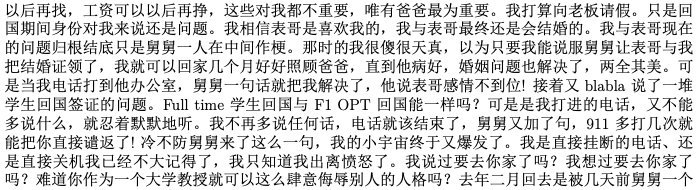
\includegraphics[width=.9\linewidth]{./pic/p1p76.png}
\end{center}

我对感情的认识很简单,总经为像10年12月与表哥的告别、自己真正惊心魂魄到、自己心里真正认定了,便是随时都可以结婚的状态。加上8月份回去闹时表哥所给予我的坚定信念,所以爸爸病重时,我也有给舅舅打电话,问过与表哥结婚的可能性,舅舅回答我说表哥的感情不到位(我想舅舅应该说的是我的感情不到位吧)。

\begin{center}
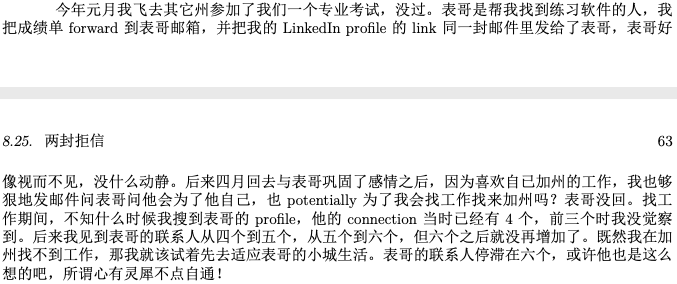
\includegraphics[width=.9\linewidth]{./pic/p1p63-1.png}
\end{center}

表哥的LinkedIn主页,对当年那个怀揣大城市梦、执拗地想要小马过河一试水深水浅、一心想要看看自己是否能在硅谷谋得一席之地的自己,是漫漫岁月里最温情的长情陪伴。

\begin{center}
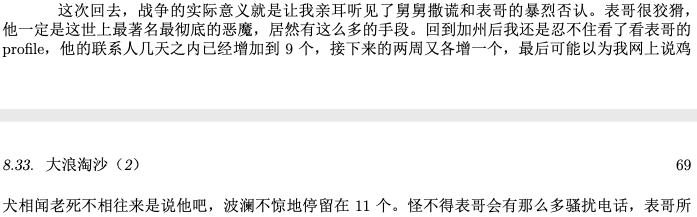
\includegraphics[width=.9\linewidth]{./pic/p1p69-1.png}
\end{center}

而8月头我心怀仇恨、怒气冲冲地杀回去找舅舅报仇恨、舅舅真的播打了911报警、而我这里却从回家看一场、从内心里从此认定了自己与表哥的感情、从舅舅家回来回到加州后,就看见表哥的主页里联系人从6个很快地涨到11个,几天之内就涨了近一倍。 

后来,我找到工作,新的工作签在中介,直接工作是家附近一家大公司Paypal.工作合同一年,中介帮办工作身份。所以身份问题最终解决下来。 

\begin{center}
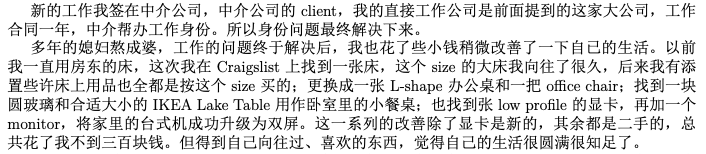
\includegraphics[width=.9\linewidth]{./pic/p1p102.png}
\end{center}

这次我见到表哥LinkedIn主页的名字又变了,变成了Eric Shing-suan Wang,就是把表哥的中文名字全拼心选加入到了英文名之间。表哥的名字王心选,心选,不只是说有心选择的一个国家,更多的应该是说,他的工作、生活、他的爱情婚姻自主吧——我走心选择了我亲爱的表哥,另一方面,表哥也用心选择了我!

\begin{center}
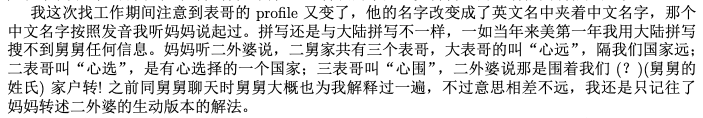
\includegraphics[width=.9\linewidth]{./pic/p1p102-2.png}
\end{center}

\begin{center}
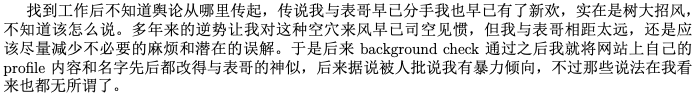
\includegraphics[width=.9\linewidth]{./pic/p1p102-3.png}
\end{center}

这里我们可以看见,在我工作的当时(一如之前奥克兰工作三个月、后来的三星公司实习11周、或后来17年工作期间,及至后来非专业职场、现实生活中总是有三大的托儿无孔不入地扰乱,非常烦恼,现在已然是弄到自己对这个硅谷心生厌倦)三大的舆论针对个人(针对他们将来的被逼性奴)总是如影随形。

最后在paypal的这份工作与表姐闹翻:我的名字改成与表哥神似

\begin{center}
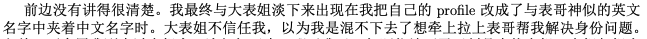
\includegraphics[width=.9\linewidth]{./pic/p1p123-2.png}
\end{center}

拿到正式的工作offer后,我第一时间给表哥写了信

\begin{center}
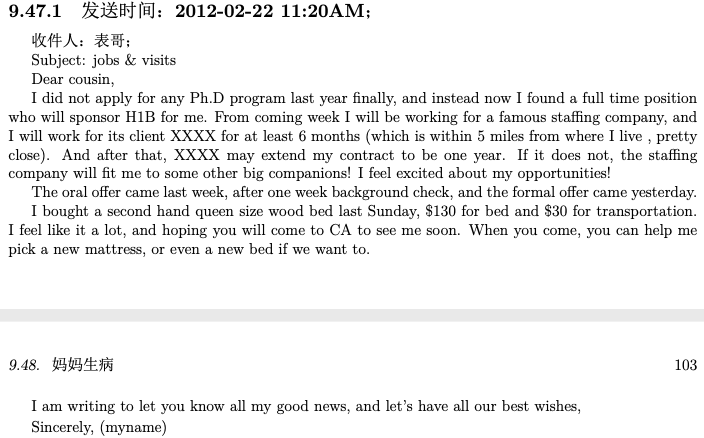
\includegraphics[width=.9\linewidth]{./pic/p1p103.png}
\end{center}

可惜他还是同以前我写给他和舅舅的邮件一样,他总是不太肯理我。 

\section{我和表哥(15)—— 职场护航}
\label{sec:org7238fcd}

\begin{center}
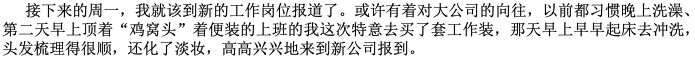
\includegraphics[width=.9\linewidth]{./pic/p1p103-2.png}
\end{center}

慢慢慢,姑娘你要干嘛?想多了啦。曾经对大城市、对硅谷有过想法,就能体会向往过、得到一份可以得到工作签证、并且自己喜欢的工作真正得到了的开心。 

上班第一天,几个账户申请下来,上班的第一天就显得轻松。 没有想到一个星期都没有理我的表哥这次在我上班的第一天给我发来了货电: 

\begin{center}
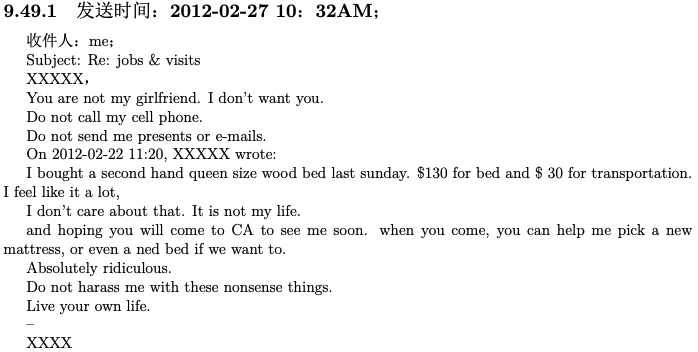
\includegraphics[width=.9\linewidth]{./pic/p1p104-2.png}
\end{center}

如果说8月份我回去,心里十二分地确定表哥是喜欢我的,那么今天读到这封邮件的时候,我心里就清楚地明白,表哥希望我喜欢自己的工作、走自己的路,表哥希望我能得到比他更好的幸福、或者有更好的成长与成熟。表哥应该是能够清楚地知道我对他的依赖吧,或许表哥希望我能够独立一点儿。 但不管表哥到底是怎么想的,现在还不能、还不愿意承认我在他心目中的位置,但他一定是真心真意、全心全意喜欢我的!

\begin{center}
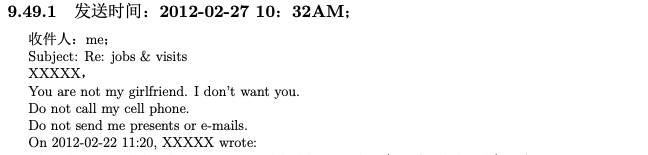
\includegraphics[width=.9\linewidth]{./pic/p1p104-1.png}
\end{center}

上班第一天两个小时之内就收到表哥的邮件贺电,我心里除了开心还是开心!

上班的第一天,后来的时候,老板也有告诉我说,这个项目是三个月的,这与中介所告诉我的是不同的。 

\begin{center}
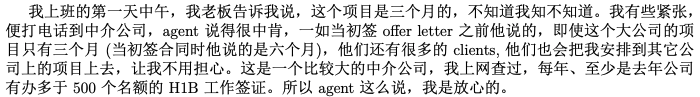
\includegraphics[width=.9\linewidth]{./pic/p1p105-1.png}
\end{center}

与中介电话里交流过之后,他们确定会给我办工作签证,所以我暂时放下心来。 

\begin{center}
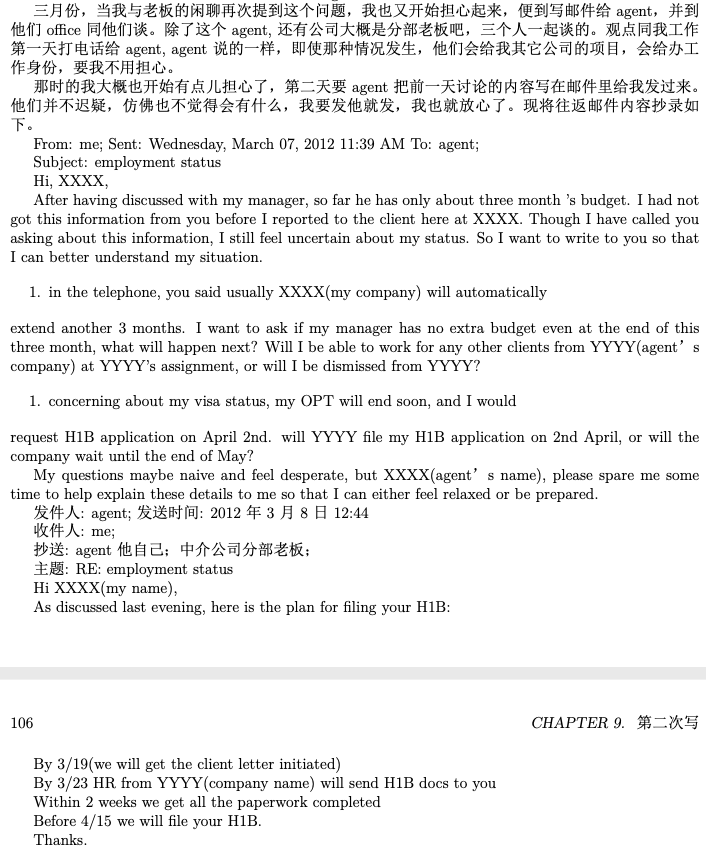
\includegraphics[width=.9\linewidth]{./pic/p1p105.png}
\end{center}

三月中旬的时候,我再次与中介确认过这件事情,并请中介作出了他们保证内容的邮件纪录。 

\section{那些年的三大舆论场}
\label{sec:orgd04df3f}

10年12月至11年2月的舆论: 我对于那时的三大舆论场是没什么认识的,只是出于自己爱情的本能更多的是顺自己的心意行事。 

不过,前面提到的初入职场时那个成名找我玩儿,那会儿的三大舆论环境,我猜测应该是自己已经被三大自己人内部人肉、还没有发动三大枪手炒作、还没有大范围舆论操控对我进行包装和封锁人生。记得最清楚的是他们内部先人肉确定这个目标时,有一次大概是炒到说我是小三什么的,当时正在上班我的情绪崩溃,跑到办公楼外面去哭。那里还没有到10年12月,还没回家见表哥呢。但那件事后,我也还是没能在意,那个每天熙熙攘攘的三大到底在炒个什么劲儿!

\begin{center}
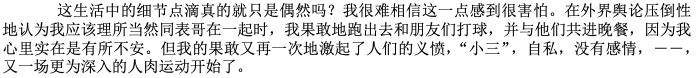
\includegraphics[width=.9\linewidth]{./pic/p1p46-2.png}
\end{center}

其实早在10年12月我回学校去协OPT之前,三大舆论早已经盯上了我,(至于最早是什么时候盯上我的,我不是很清楚,没有那份敏感和判断力),因为他们早就在炒说我天天在加州找朋友,最后发现男朋友在舅舅家在自家后院,实则是说表哥在他学校这么可能等得有些着急,表哥可能他自己在家里单方面曾经采取过什么行动吧?! 

\begin{center}
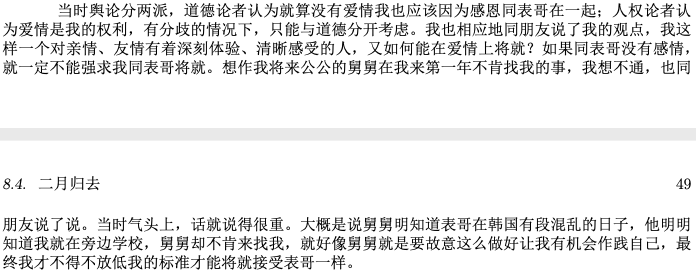
\includegraphics[width=.9\linewidth]{./pic/p1p49-2.png}
\end{center}

其实所谓当时的舆论分为两派,更多的、更本质的应该是三大为了炒作一个人,他们炒作团队内部把观点分成了两派,以便到时至少有一派是能够最终成立的,并能在他们三大内部先把这个人人肉一遍,所谓选定炒作目标的步骤,随时做好准备发动网络炒作并封锁当事人人生的状态。

舅舅打911后我回到加州的情况是: 舆论已经把人赌成出不了门、上不了班的地步。 

\begin{center}
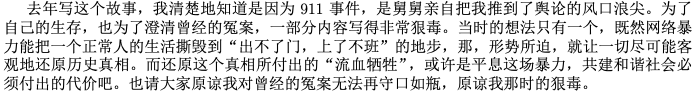
\includegraphics[width=.9\linewidth]{./pic/p1p75-1.png}
\end{center}

\begin{center}
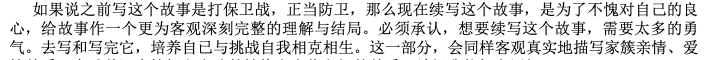
\includegraphics[width=.9\linewidth]{./pic/p1p75-2.png}
\end{center}

所以后来,8月头回去找舅舅发泄仇恨的三个月后,我已经是被逼得没有办法,11月4日,已经只能站出来写自己《成长的故事》了。

\begin{center}
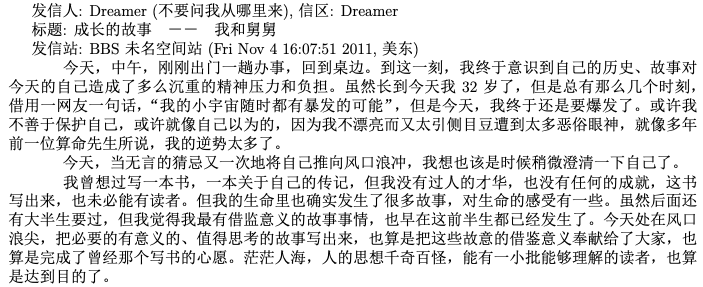
\includegraphics[width=.9\linewidth]{./pic/p1p9.png}
\end{center}

事情也很奇怪,11年2月我被第一份工作的公司解扉,被推到了后来备受伤害的奥克兰三个月的工作,后来无果我被解扉。第一份工作的公司给我续做了三个月,到12年1月。

一年后的12年1月,我再次被第一份工作的公司解雇,继而被推到了12年2月的中介公司,我便有了职场上唯独一次(Once in a life time)表哥对我貌离神合的珍贵随行陪伴。

\section{成长的故事 -- 我和表哥}
\label{sec:orgfb61514}
\begin{itemize}
\item 2011年11月4日,当三大中文媒体对我的人肉已经伤及我自身生活,我必须站出来澄清自己, in Part 1, (San Jose, CA);

\begin{center}
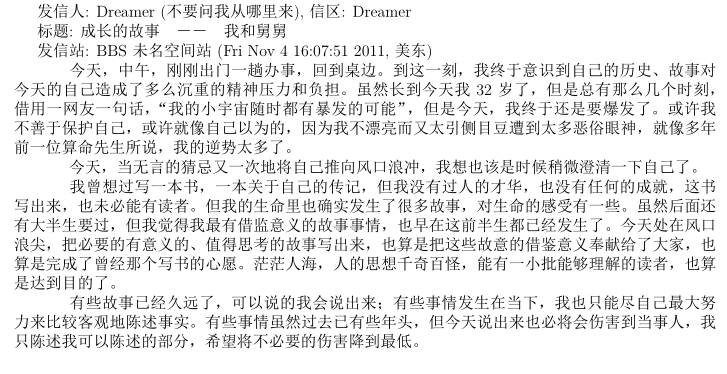
\includegraphics[width=.9\linewidth]{./pic/dreamer1.png}
\end{center}
\item 4/19/2012 - 6/17/2012, in Part 1, 第二次写至统计专业OPT实习结束(San Jose, CA);

\begin{center}
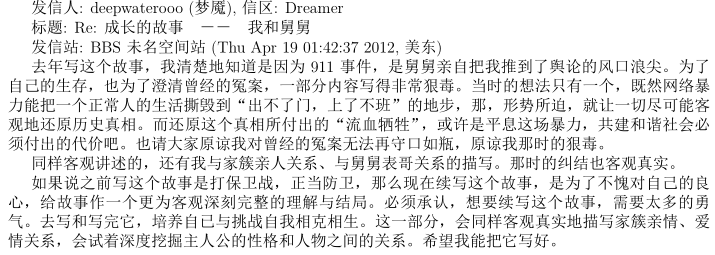
\includegraphics[width=.9\linewidth]{./pic/dreamer2.png}
\end{center}
\item 2014年夏天,写于SJSU Library (San Jose State University Public Library, San Jose, CA)

\begin{center}
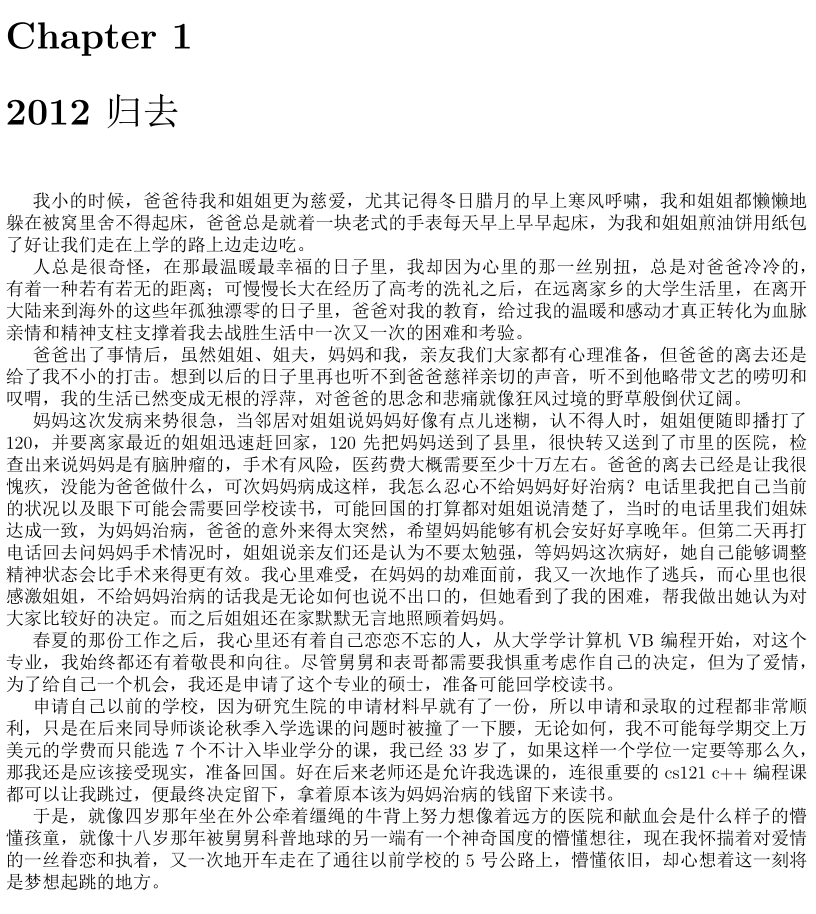
\includegraphics[width=.9\linewidth]{./pic/dreamer30.png}
\end{center}
\item 2/13/2015 - 12/17/2015(?, Moscow, ID; either and or not San Jose State University Public Library, San Jose, CA)

\begin{center}
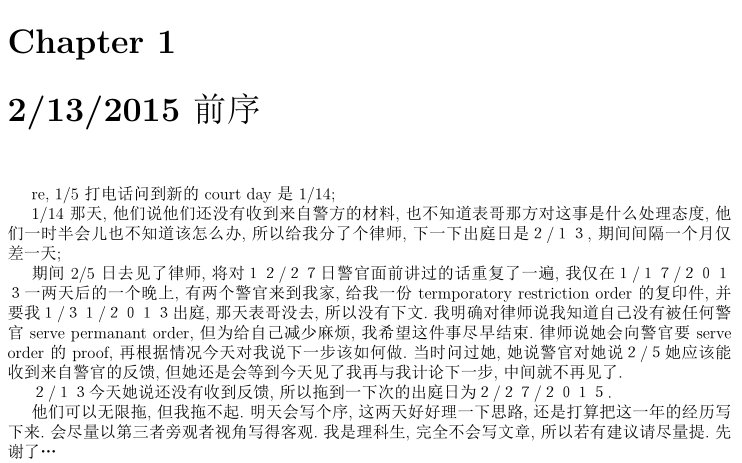
\includegraphics[width=.9\linewidth]{./pic/dreamer3.png}
\end{center}

\item I will reorganize the four pdfs, and emphasize keys issues and situations of the whole process, while at the same time to help major population understand what's going on, and what's inside opinions. 虽然这个成长的故事系列是以2011年当三大中文网站(mitbbs.com, wenxuecity.com and backchina.com)中文媒体对我的人肉与网上评论伤及我的正常生活时,我站出来开始写自己的自传,并分四次在四个不同的时间段,不同舆论或事件压力下或是网上澄清,或是网上求助以便能帮我泄掉一部分当时自己的压力,分四次于不同的地点纪录了的自己的主要生活,纪录到2015年计算机硕士学位结束。
\item 这一次,这里,我会以事件主要人物及其相关主要事迹的人物列传、或/和大事记、大冲突记的形式来重新组织语言,重述我的整个成长史与大事记、大冲突记,来帮助自己成长、并帮助社会大众认清事情所有环节真相的目的。但鉴于时间有限,我会以剧情梗概的形式每天大致纪录与一个相关人物某件或某几件事的进展、或一天一两个主要事件,并将已经完成了的四个部分作为原始事件纪录的细节参考供索引,并争取做到每日更新一篇,到我把先前与这个教授舅舅的所有冲突的这件事情具体讲述清楚,以供大家共同去探讨事情的真相到底如何,有一个更能为大家所接受或理解的底层社会小人物的心灵成长史。
\end{itemize}

\section{我和舅舅}
\label{sec:orgd4dac31}

我生在一个农村家庭,家里上面有三个姐姐,我是家里最小的,很乖很听话,我从小爸妈都比较宠我,尤其是爸爸,三姐也常私下报复我嫌爸爸把我宠得连点儿样子气儿都没了!上小学之前还要家里伯伯家堂叔的照看下跟着他一起给家里放过两年牛。 

我们家爷爷走得比较早,我们姊妹从来不曾见过爷爷。爸爸对奶奶极为孝顺。爸爸有弟兄三人,长大后听妈妈说起,叔叔家结婚后很长时间没有孩子(,没办法只能后来领养了一个。),奶奶受旧社会观念的束缚,认为没有孩子是很大的罪过,指挥起了爸爸。爸爸对奶奶太孝顺了,只是一味地听从奶奶的话,却背叛了妈妈。妈妈受到伤害,没能及时原谅爸爸,家里两个大人就常常吵架。我那个时候大概只有五岁左右,什么也不懂,本能地觉得是爸爸错了,同爸爸的心理距离比较远,大多时候与妈妈比较亲一点儿。最小的姐姐三姐只比我大两岁。我不知道他们吵架的时候,姐姐在做什么,我就常常躲在被子里哭。

小时候,我耳朵生脓,爸爸有带我看过村里的医生,因为是外部受感染,一般擦些药就好了。只是不知道为什么,我的耳朵总是会出脓,也试过偏方,就是把一种很特别的幼小稚嫩植物的茎挤出汁来擦进耳朵,但却还是总是有脓,这样持续了很长一段时间。后来长大后在一次上课老师测试大家的听力时,我竟然发现我的听力比同班同学差很多。 

可能是随了妈妈的基因,还算人不太笨,从小到大的学习成绩一直都还是不错的。小学的时候比较贪玩,一般平时就考个年级前三名。小学时候也有自己喜欢的人,我是属羊的狮子座,进一年级的时候班上来了三个复读书,其中一个男生,个儿高高的,属马热情大方,我猜他是白羊座,小学六年就成了暗恋这个男生的六年,同他所在村子的小伙伴们每天一起上学放学回家两次,听他们聊各种电视剧。而每当早读要背书时,只要是他要到我这个组长这里来背书,我就一定会捉弄他,鸡蛋里挑骨头,不让他一次背过,好让他每次早上要背书都要他来我这里多背上几次到快下早读为止。

我上小学的时候家里最大的姐姐已经开始相亲谈恋爱了。妈妈总是把家里收拾得干干净净,姐姐领了朋友回家,爹妈就会做可口丰盛的饭菜款待客人,从大姐谈恋爱开始,我就一直认为爸妈偏心,喜欢大姐,而我和三姐这些小的,尤其是我这个最小的,穿衣服就只有捡她们穿旧穿小了的旧吊吊,心里当然不平。

小学快毕业时候的一件意外性侵扰事件让自从上了初中的我被背负着沉重的精神压力,观察自己身体发育的变化,与同班的女同学们相比,想起自己有个后来领养了孩子的叔叔婶婶,我自己心里一直非常担心自己将来没有生育能力。可是爸妈又一直都很偏心大姐,以至于小时候成长的观念里就没有爸妈是自己这个世界上最值得信任的人这个概念,便就没把这事告诉爹妈,一个人心里压着。到上初中了,爸妈就对我的学习管得紧一点儿,虽然心里压着事儿,可初中文化课简单,初三时因为自己学习好又交到了一个比较交心的女同学朋友,到初中升高中中考时我的成绩就成了全镇文化课的第一名。

\begin{center}
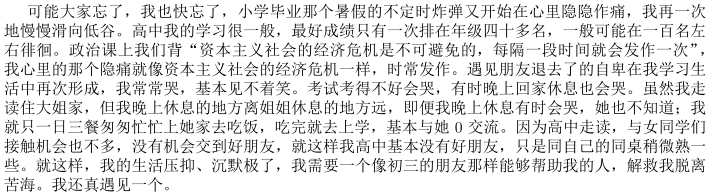
\includegraphics[width=.9\linewidth]{./pic/p1p21-0.png}
\end{center}

初中两三年里,那件事我基本一个人就抗下来了,可是这也并不是说我高中就能同样抗得下来。高中课业比较重的情况下,我心里再担着事儿,个性就比较压抑,直到1997年的夏天,我18岁时,遇见了回国探亲的舅舅。

\begin{center}
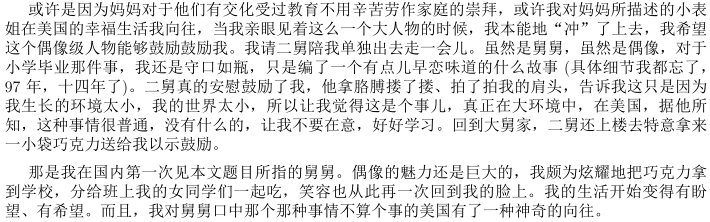
\includegraphics[width=.9\linewidth]{./pic/p1p21.png}
\end{center}

一直觉得爸妈偏心,没有把那件事告诉爸妈的我,遇见舅舅后,我把这件事告诉了舅舅(请原谅我,我真的不记得我当时到底对舅舅说的是什么事了,但我真的得到了鼓励,能做到把担心自己将来能不能生小孩的事暂时放下)。他安慰我说没事,不用担心,现在只要好好学习就可以了。舅舅说在农村环境里长大,会对家里的小动物、植物等都有着纯天然的热爱。舅舅建议我说将来不防读农林院校,一辈子如果能在学校里研究研究这些植物搞搞科研,看看能不能让苹果树结出其它口味的苹果什么的,也会是一件很有意义的事。舅舅陪着我走,聊了聊其它的,又把我领到大舅大舅母家,从他衣箱里拿出一袋传统的巧克力糖,鼓励我丢下包袱,好好学习。

见到过舅舅后,我并没能完全丢弃掉我担心自己将来不能生小孩的事,但我学会了放下,可以把这件事将来该考虑的时候再考虑。高三的时候,我的同班同学们发现,那个从来不笑的女孩子会笑了!

而我之前听妈妈说起过一直羡慕大舅家的小表姐(Cindy Wang)上高中就被叔叔带到美国去读高中,我此前也有对班主任老师说过我有个美国舅舅会把我带去读书。后来高三即将高考的春季,当班上舆论发酵说这个女孩子早恋的时候,长年来性格比较孤僻的我人生中第一次经历如此大的打击,我被这次暴发的舆论打倒了,他们说我早不早恋的我都没关系没所谓,我意识到了自己不该撒谎,那时极度脆弱的我把自己给打倒了!

姐姐把我领回农村老家交到了爸妈的手上。那时农忙刚结束,早年经历过离婚和几年浪子生涯的爸爸内心里肯定还是受到过震撼,他只留自己在老家忙田地里剩下的农活,要妈妈陪我去姐姐家住着,把我给看管好了。就这样我又重新回到了学校。我的思考并没有因为妈妈的到来而结束。这一次,到这种情况下,我终于一个人撑不住了,所有发生过的事情、那里心里的想法统统向妈妈、姐姐们一一交待清楚。学医的二姐告诉我,人只有在三种情况下不能怀孕:精子存活率过低;精子卵子不能结合成受精卵;受精卵不能成功着陆,并分条一一向我解释清楚;二姐也从客观事实和科学的角度向我解释了叔叔家不能生先领养了一个孩子,后来妈妈说婶婶是引子伢子后来又生了一个,但其实并不是叔叔的孩子(并从科学与事实的反复对照让我明白妈妈说过的引子伢子从来都只是她个人的社会观察,没有任何科学依据)。姐夫向我举例说明算命先生的话可以有多种理解,他们是见风使舵的主儿。妈妈也找到了姨父问了那次有个算命先生到他家里到底是怎么回事;他们尽了他们能尽的一切努力想要说服我,但我实在是太绝望了。

\begin{center}
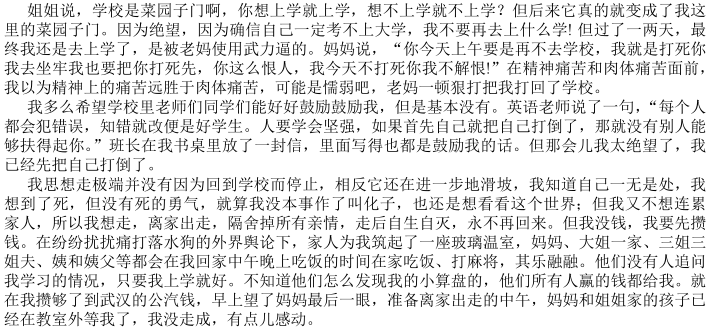
\includegraphics[width=.9\linewidth]{./pic/p1p22-1.png}
\end{center}

在妈妈的看管下,后来我勉强考完了高考,也听取了舅舅一年前的建议,报考了农林院校,考完后就一直呆在农村老家静养。

亲人里没有任何人再问我成绩相关的任何事。等有一天,我自己想通,怕高考没有考好考不上大学的时候,我对爸爸说,如果这次没有考好,我还想再复读一年再考一次!这一次,我看见了爸爸的期望与感动,他说好!

\begin{center}
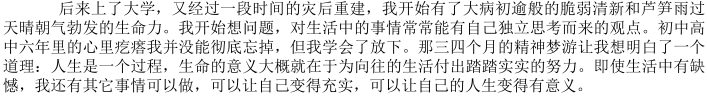
\includegraphics[width=.9\linewidth]{./pic/p1p23.png}
\end{center}

上大学后读了农林院校的我了解到这个专业还是比较容易出去的,便好好学英语,其它科目倒不是很在意。到大三下学期,即将面临一年后1月份的硕士研究生考试,如果再不考TOEFL等英语考试,这个想出去的梦还要拖到什么时候呢?可是这个时候基本没有任何项目经验的我直接申请国外的硕士研究生也是很难(基本为0)拿到奖学金的。当理想与现实有着巨大的落差,大三下学期的我,就很焦躁,下课后跟同学一起走回宿舍的我曾对同寝室的女孩薇说,我感觉自己现在就像是空气中舞动的尘埃,每天最想做的事就是赶快回寝室,赶快冲到水龙头下,好好冲上半个小时,好把自己变得滋润清新。

\begin{center}
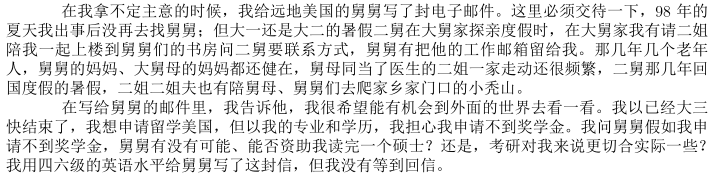
\includegraphics[width=.9\linewidth]{./pic/p1p25.png}
\end{center}

大三下的春夏,我的纠结、浮躁迟迟不能尘埃落定。但一场病、一个手术结束了我的痛苦选择。当我因阑尾炎手术住院二姐二姐夫来医院看我的时候,我告诉了他们我的想法。二姐夫说我心比天高,命比纸薄,能考个国内的研究生就不错了。于是我以刚好压线的成绩考到了北京的农科院。

\begin{center}
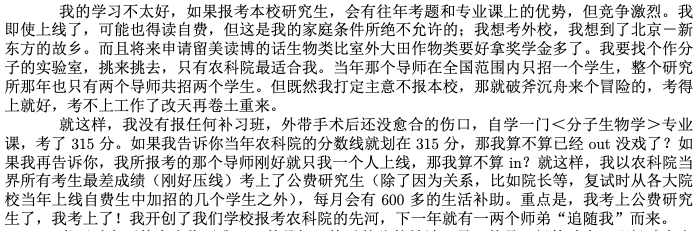
\includegraphics[width=.9\linewidth]{./pic/p1p26.png}
\end{center}

在北京硕士的三四年时间,我也顺利地通过了必要的英语考试,申请到这边一所学校里读书。期间有经历过一次感情的伤害。

2006年金秋8月,我二姐与二姐夫暂借我\$1600作为最初最基本的生活开销,我踏上了这片向往了近十年的自由国度的热土,开始了我的国际留学生生涯。

第二年(2007年5月),一次电话里二姐把我骂醒,我从过去的感情伤害的阴影中走出来之后,终于感觉到了春夏的阳光灿烂。

我曾用它写邮件给过舅舅、后来又被我遗忘了的舅舅工作单位电子邮箱里的“eecs”四个字母就像一串神奇的密码崩入了我的脑海!舅舅工作单位电子工程与计算机研究院网页中几十位教授的照片里,我一眼就认出了舅舅。 舅舅的办公室是在sloan 321,看了他的这个周的office hour的时间。那时我们University of Idaho与Washington State University之间为方便学生交差选课,还在免费公交大巴车可以乘坐,我迫不及待地第一时间赶到了舅舅的办公室,有个学生正在请教舅舅课业上的问题。 

舅舅的办公室里有他捣鼓各种电子零部件堆积着的桌面,和一张B5纸打印出来的他的亲侄女、我的表姐王夏华的大副黑白大头照。请教问题的学生很友善地很快离开了,我叫了舅舅,在美国与舅舅又一次地认了亲。

\textbf{备注:}

在这前后不到一周五天左右的时间里,我这过去十年来几乎第一次去读的我十年前写的关于自己人生亲身经历的传记,却突然发现很大一部分的记忆正在从我的脑海中流失,还停留在记忆里的是那些最最感动过我、触动过我的深刻记忆。可能儿时的经历里受到过损失的并不只是我两只耳朵的听力,还可能有关于记忆力发育与受损的版块。

这第一次写自己早期人生中最痛苦的经历,虽然事件本身早已成为过去,但在读与回忆里,在重新总结时,仍会禁不住掉很多眼泪,稍微休息不好,头就会很痛。以后写其它部分,应该会比这一篇回忆容易轻松很多。我原本是打算把美国这边与舅舅的交往再能记起的,在这一篇里都写出来的。但我还没有想好到底要写几篇,与舅舅,与表哥,官司纠葛、职场等,要写多久,一个星期可能比较困难,半个月也说不定,可能半个月左右吧。对于如何组织构篇,如何往后推进,我还要再想一想。

\section{我和表哥}
\label{sec:orge572e5a}

2006年一学年,我是没有手机没有电话,朋友也是比较少的。后来意识到在恋爱结婚年龄,我是需要多交友的,于是2007年秋季有新生入学时就早早地与新学年学生联系,组一个family plan,来拓展自己的交友范围。同期,应该与有与国内的自己以前的同学等电话联系。2008年夏天我是最有热情和冲动想要暑假回国,回去见见自己的父母,也见见自己的老同学。2008年春天与舅舅的某次见面中,我有问舅舅一个问题,我有一个国内同学,我也还比较喜欢(是我高三元旦在我课桌里放贺卡那人)。我们也还有联系,感觉可能大家也都还有意思,我问舅舅,这种情况,我可以暑假回去见他,看有没有可能解决自己的个人问题吗?舅舅首先问了我,“他离婚了吗?”我答“应该还没有”。舅舅说那就让他先把婚离了再说。我惊异于舅舅的犀利透彻,人家婚都还没有离,就算那同学与我现在互相还有那么一点儿意思,他不离婚也就犯不着我现在要怎么样!

紧接着舅舅就告诉我,这个暑假(2008年暑假)我们要去加州,他要带我去那边都会我如何用非专业相关的工作为自己挣些学费和生活费。

于是,接下来的2008年寒假,以及2009年暑假,我都在加州硅谷度过。2009年初夏去加州,走之前舅舅问我,这是最后一个学期了吗?还可以再延期吗?我告诉舅舅我已经申请秋季学期毕业了。09年暑期结束,当我回到学校,发现舅舅把我那个传说中呆在韩国好多年的二表哥王心选给搬回来了。

8月,舅舅邀我去他们家作客吃晚餐,我第一次见到了舅舅家的这位二表哥,与表哥同时出现在我的世界的,还有舅母。

早期的留学经历过了这十多年,在我这几年脑海里的记忆已经所剩不多,包括很多那些年与舅舅聊天的无关无重的锁碎细节,甚至包括某次从硅谷回到学校时我写邮件告诉舅舅我回来了,但因为时间急,这次回来没有给他带礼物时,舅舅那句曾经深深感动过我的回信只有两个词的那句Welcome home!”(这几天第一次回去重读,才想起来,但我现在想不起来08年底有坐飞机去过哪里?还是当时是开车,自己笔误写错了?)。

\begin{center}
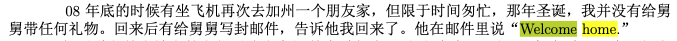
\includegraphics[width=.9\linewidth]{./pic/p1p34.png}
\end{center}

在我现在记忆的深深深处,在舅舅第一次把我带到他家的那次,我记得站在厨房厅里,我看到的是舅舅那儿,他们家的门窗桌椅等都用稍厚的塑料包裹把整个家的门窗桌椅家具等都保护得极好的一片塑料世界!(至此,我终于意识到,现在四个文件应该至少是在2013年秋天当我学会用Emacs Latex auto generate and export pdf之后从自己电脑上仍保存的文稿合并的。但2011年4月,2012年春天写的当时发布在mitbbs.com Dreamer版面的内容应该更多,而现存在于这四个文件中的只是原始最初发布在网上所有内容中的一部分,也就是,当时发布在网上的内容,我现存的,现在仓库里是有缺失的,现仓库里的内容不够完整)

这次再到舅舅家,那些起保护作用的诸多的塑料已经被舅舅全都收起来,正常人家的装饰与摆设。

及至吃饭时,再见到舅舅的这位表哥,我们像是在哪里见过,兄妹间有种深入骨髓相亲相爱的亲密亲近。

2010年12月,长途车开回家,那天晚上见过表哥后,我也就早早休息。第二天起床后,见家里是一座空城,便问舅母表哥在哪里?舅母说你去舅舅办公室找到舅舅,你就能找到表哥。记不清什么情况下问的舅母了,舅舅一把年级了,周末晚上什么的还要经常去办公室吗?舅母告诉我,舅舅在写一本书。我想起之前同舅舅聊天时什么情况下聊起的,我曾同舅舅聊起说过,我想写一本书,一本关于自己的书。

我如同2007年夏天当我从过往的感情伤害中走出,eecs成为一串神奇的秘密崩入我的脑海,在舅舅院系主页里我找到舅舅的办公室门牌号321,来到舅舅的办公室,我在美国第一次找到了舅舅。那天早上,我听从舅母的建议,又一次地去到舅舅的这个321的办公室,我找到了我生命中的表哥。

舅舅在做他的事,我表达来意后,舅舅曾郑重地向我说过:你相信舅舅,就可以相信表哥。舅舅带我来到表哥的 student office, 表哥看见我就先笑了。表哥身材高挑,皮肤白皙,深隧的双眸清彻见底,身形眼神都像极了我小时候那个极其宠爱我的父亲。

表哥和我打算去图书馆找一个我需要用到的软件。

\begin{center}
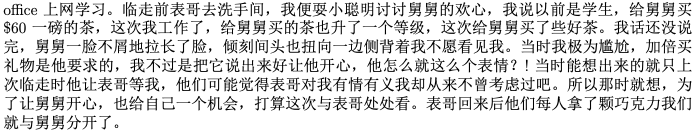
\includegraphics[width=.9\linewidth]{./pic/p1p41.png}
\end{center}

舅舅走前也要求过我,同表哥帮我办完事后,回舅舅那里去学习,要我不要打扰表哥。

办完事后,我早已把舅舅要求我回他办公室学习的话忘到了九宵云外,在表哥那里呆下来。

知道表哥是属马双子座的,我问了表哥的血型,表哥说他是O型血。我满足了,跑回去自己上网。

过了会儿又跑回来问表哥,中午我约了和以前学校里的几个朋友一起吃顿饭,表哥可不可以陪我一起去,表哥同意了。 

过了会儿又跑回来问表哥,表哥这里有没有什么好玩儿了?表哥说好玩儿的呀,就打开一个放满照片的文件夹,我也搬把椅子坐到表哥右手边,表哥就给我讲起那些动物园里的小动物来。表哥给我讲了园子里斑马与孙雀的故事。表哥说,他们在一个园子里相处得久了,他们之间不说什么、不做什么行动上也有了默契。表哥给我讲他拍到那张照片时的情景。表哥说最开始那只孔雀只是在一边远远地站着,斑马朝孔雀的方向走过来。眼见着斑马就要遇见孔雀了,没有早一步,也没有晚一步,孔雀只挪动一小步就避开了。没有想到我的生长于美国的表哥还可以用中文讲出这么好玩儿的故事。

表哥给我看了些其它的动物照片,并从另一个文件夹里打开一些大表哥家两个小孩儿的照片给我看,他们都很可爱。现在才想起,在09年秋天舅舅邀请我到他家作客时,餐桌上舅舅就对我们讲过关于小动物的事情,我竟是忘了。

表哥讲说他出差,去动物园看过那些小动物持,曾走过很远的路,拿到两颗免费的糖。表哥边说边走近他的小冰箱,拿出一小袋里面只有两颗、装在一个充了气鼓啷啷的塑料袋里的巧克力给我。我接过来拿在手里揣摩端祥着,当时确实有向表哥表白并吃掉一颗的冲动,但这一切对我来说还是太快了,我还得再想想,便很无奈地把巧克力糖原封不动地还给了表哥。或许表哥曾热切地注视过我,或许他真的失望了,折回来后,我们还坐在并排的椅子上,椅子之间相隔的距离也 不曾改变,但表哥开始写他的code,有一种明显的台风过境的疏离。我是自私的,即便我现在还没有想好会与表哥发展成什么样,但我是喜欢表哥的,我怎能容许表哥现在就这么从我的世界里消失掉?!就算没有表白、没有勇气打开这个对表哥来说意义如此重大的巧克力糖,我也不允许他走掉。我双手抓住了下表哥的右胳膊,他不理我,继续写他的 code,我也不曾放手。我当时心里就只有一个想法,我是真诚地喜欢着表哥的,所以我什么都不用怕,我的两手交差就继续往下抓,他不动我还抓,从大胳膊顺势往下抓到了他右手,又用另一只手抓住了他的左手,并把我们的四只手合拢到一起。这下他满意了,很开心地说,“我们去吃饭。”没有因为自己的不小心把表哥放跑,我很开心。

我们去吃过饭,告诉表哥我想上厕所,表哥带我去图书馆。我把外套留给表哥帮我拿着。我感觉自己并不慢,但出来时看见一胳膊上搭着我外套的表哥橱窗前站着边看橱窗边等我的意境感觉很美。

早上去图书馆找我软件相关的东西时,我曾看见掉落在地上的一张白色长方形卡片,不知道是作什么用会掉在地上,我伸手把它拾起来,放在了旁边的坐位上。我喜欢大学四年里武汉的雨水,曾深深滋润过我的心灵。我喜欢同表哥一起走在大学校园的小道上,芳草戚戚,滋润清新,表哥把一路上他能看见的垃圾也都捡起来,我们眼中的世界干净清辙又纯粹!

等我们回到表哥的实验室,我的事情都已办完,舅母说她上午用洗手间,我下午可以回去洗澡,我想先回去洗澡了,便同表哥打好招呼自己先回去了。 

舅母在橱房里准备做菜,舅母说这炉子还有点儿小姐脾气,时好时不好的。

舅母说起家附近一个什么类似”工厂”的地方, 表哥毕业后,舅母说希望他就在附近能在那里上班就好。舅母给我讲那时候她对表哥非常严格,从来都要求他自强自立,从多大起就自己攒钱养活自 己。舅母说因一件什么对表哥用钱格外苛刻的事她现在还有点儿后悔,如果当初她不对表哥有那么严 格,表哥或许不会远走他乡(具体是不是远走他乡,是什么事情其实我没明白透)。

那天傍晚表哥晚了一个小时才回家吃饭,我想可能表哥觉得我走的时候同他说的那句“表哥我先加去,你晚上早点儿回来”他听出什么别的意思吧,也没有多想。想一想,我硕士时曾有一个住宿舍对面的朋友,是我一生中最为要好的两个朋友之一,另一个是初三时候的孔雀女朋友睿。这个朋友属马双子女O型血,她的世界很单纯并喜欢我比较单纯的个性,她说过她和我作朋友只是因为我单纯,从来没有任何的坏心眼去害别人。她也对我说过,“小黄,你知道吗,你身上最宝贵的品质就是善良,不管遇到什么困难,不管在社会上经历过多少磨难,你都要保存保护好这一点,永远不要失去它。”我在想,比这个朋友大一个轮回的表哥,作为男性,会有什么不同呢?第二天,我就找到了答案。

第二天,我自己从学校里办完事,回家收拾好行李准备离开时舅母的话侧面提醒了我,我一定要去学校再见表哥一下。表哥出来接我去他office。 Office里没有别人,我想表哥抱抱我,他不肯;我拉着表哥的手,带着哭腔说,“表哥,我晚上没休息好,我心里难受,我不想走!”蹲在地上快哭出来。表哥在给一个什么人打电话,我也管不了那么多了,靠在表哥后背上哭起来。哭了好几分钟吧难受得也快差不多了,便松开了抓着表哥的手,从后面抱住了哥哥。两的两手臂上一阵温热,哥哥还是徒然地放下了他试图掰开我的两只胳膊。我在后面嘟嘟囔囔地说,“表哥,我觉得接下来的一年好辛苦!”边说边把侧靠着的头调了个方向,就这样静静地抱着。我还有要紧话要对表哥说,便转到前面来,表哥这次也不再躲闪,顺着我,我顺势双手从前面揽住了他的腰,面对面身体贴着他说出了我俩之间最亲密的话,“表哥你喜欢我吗?”“我把你当妹妹。”没防备表哥会说话,话音刚落,“可是如果我也喜欢你呢”我的话已崩出来。我只好自己接着往下说,“可是我还没想好,我不知道该选什么样的人。”我接着说,“以前都是舅舅支持我,表哥,以后你要支持我、鼓励我。”表哥这里很温暖,我紧挨着表哥胸膛的头又调了个方向。

想了想我又说,“接下来的一年,我没心思谈恋爱,等我把工作换了转了身份,我会想谈恋爱,会考虑感情 问题,到那时我应该也会想清楚了。”我知道自己干了件世界上最自私的事,想了想又定定地说,“我 知道舅舅、舅母对我俩这事的态度,等我想好了,表哥,不管我有没有选你,我一定回来跟你说清楚!”为什么我会说这么多的话,为什么表哥都不肯抱我?我终于还是耐不住了,“表哥,就算你把我当妹妹,你就不能抱抱我吗?”边说边甩开原本握着的表哥的手,双手在表哥后背上忙碌起来。可是表哥还是不肯抱我,我觉得我的后背发凉。

无奈我就只能再次抽出已然插入裤衣口袋的表哥的手。表哥很温柔地说,“没休息好应该中午回去睡一下!”我智障吗?所谓“大跌眼镜”,眼珠都快掉下来描述的应该就是我当时的感受吧,想来昨晚我走时表哥听到我略带试探的话可能也是这个反应吧,所以他才拖拖拉拉很晚回家!我本能地迎向哥哥的目光,说,“基本上还能开得回去。”

这时表哥的导师进来了,我们不好意思地松开了手。“我该走了,表哥你送我出去吧!”表哥给我带错了门,“从这里出去我找不到我 的车。”表哥停下来问我,为什么接下来一年会辛苦,我就解释了一下工作的事;“要一年吗?”表哥 问得真诚真切充满期待,我知道自己干了件最自私恶毒的事,本能地想要减轻他的痛苦,答说,“半 年,大半年!”“你呆会儿还回去吗?”“不回去了。”“路上不要超速,开车要小心!”表哥带我找正门, 我们牵手了。看见第一个人时我们松开了,但终究还是紧紧地握在了一起,对走道里的学生视而不 见,世界仿佛只剩下我俩!到门口,我说,“表哥,我要走了!”“小心开车!”我扣上外套,走出了大 门。回头望时,表哥还定定地站在那里,眼里充满期待,我一阵心酸,眼底升起一股迷雾,眼前已是一片蒙胧。

\section{我和表哥(2)}
\label{sec:org5d091c2}

2010年12月的那个周一,在与表哥的那场告别里,同以往有限的几段经历一样,借着表哥与我的亲密,我原本只想表哥能够抱抱我、给我一点儿温暖和鼓励,不曾想自己当即迷失在表哥的无限宠爱里,把自己的眼泪和灵魂都永远地献给了对方,从此万劫不复,今生不得解脱,这是后话。 

在开往加州的路上,我想明白了表哥一定是喜欢我、宠着我的,他那句拿我当妹妹的话说得是那么地言不由衷。在表哥的宠爱里,我变回成幼年那个被父亲宠爱的小女孩。原来这一直是我内心里真正渴望得到的,今生我应该就跟定表哥了。 

知道自己喜欢表哥,我也有假惺惺地打电话问过舅舅我与表哥的亲缘关系,舅舅说我妈妈的爷爷与舅舅的爷爷是同一个人。我也曾假惺惺地问过舅舅他们作父母、舅舅舅母的立场。舅舅说他既不支持也不反对。电话里,舅舅在一个什么不打紧的间隙不打紧地加了一句:“他以后结婚了不要小孩都可以!”

\begin{center}
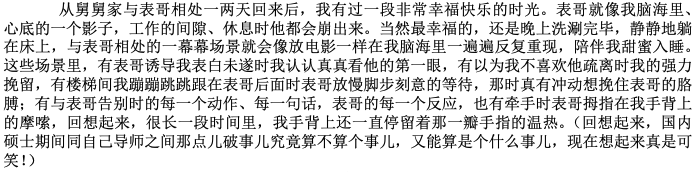
\includegraphics[width=.9\linewidth]{./pic/p1p45.png}
\end{center}

喜欢上表哥以后,我每天头脑发热,恨不得天天给表哥写邮件,想跟表哥表白。

\begin{center}
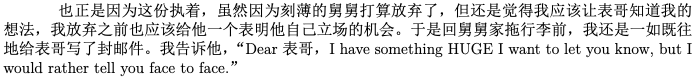
\includegraphics[width=.9\linewidth]{./pic/p1p49.png}
\end{center}

两个月后,2011年2月,我又回舅舅家了,表哥坐在我上次坐过的地毯上,锻炼的缘故,白净了很多。我拖住表哥的胳膊求他带我去超市买回去时路上需要吃的东西,一拖便知道表哥变结实了。我央求表哥带我去他的办公室,表哥不同意。就要结束了,我都还没有向表哥表白,我让表哥带我到一个我可以讲话的地方,表哥把我带到停车场息了车。

\begin{center}
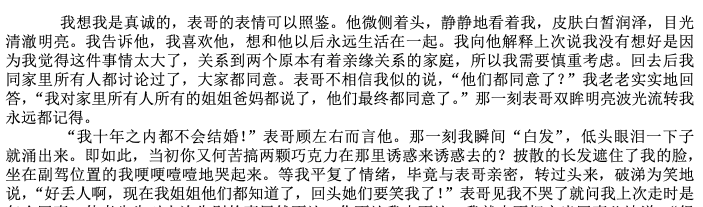
\includegraphics[width=.9\linewidth]{./pic/p1p50.png}
\end{center}

表哥带我去超市买东西的时候,门口正有工作人员在送礼物,于是表哥就送我了一枚戒指!

\begin{center}
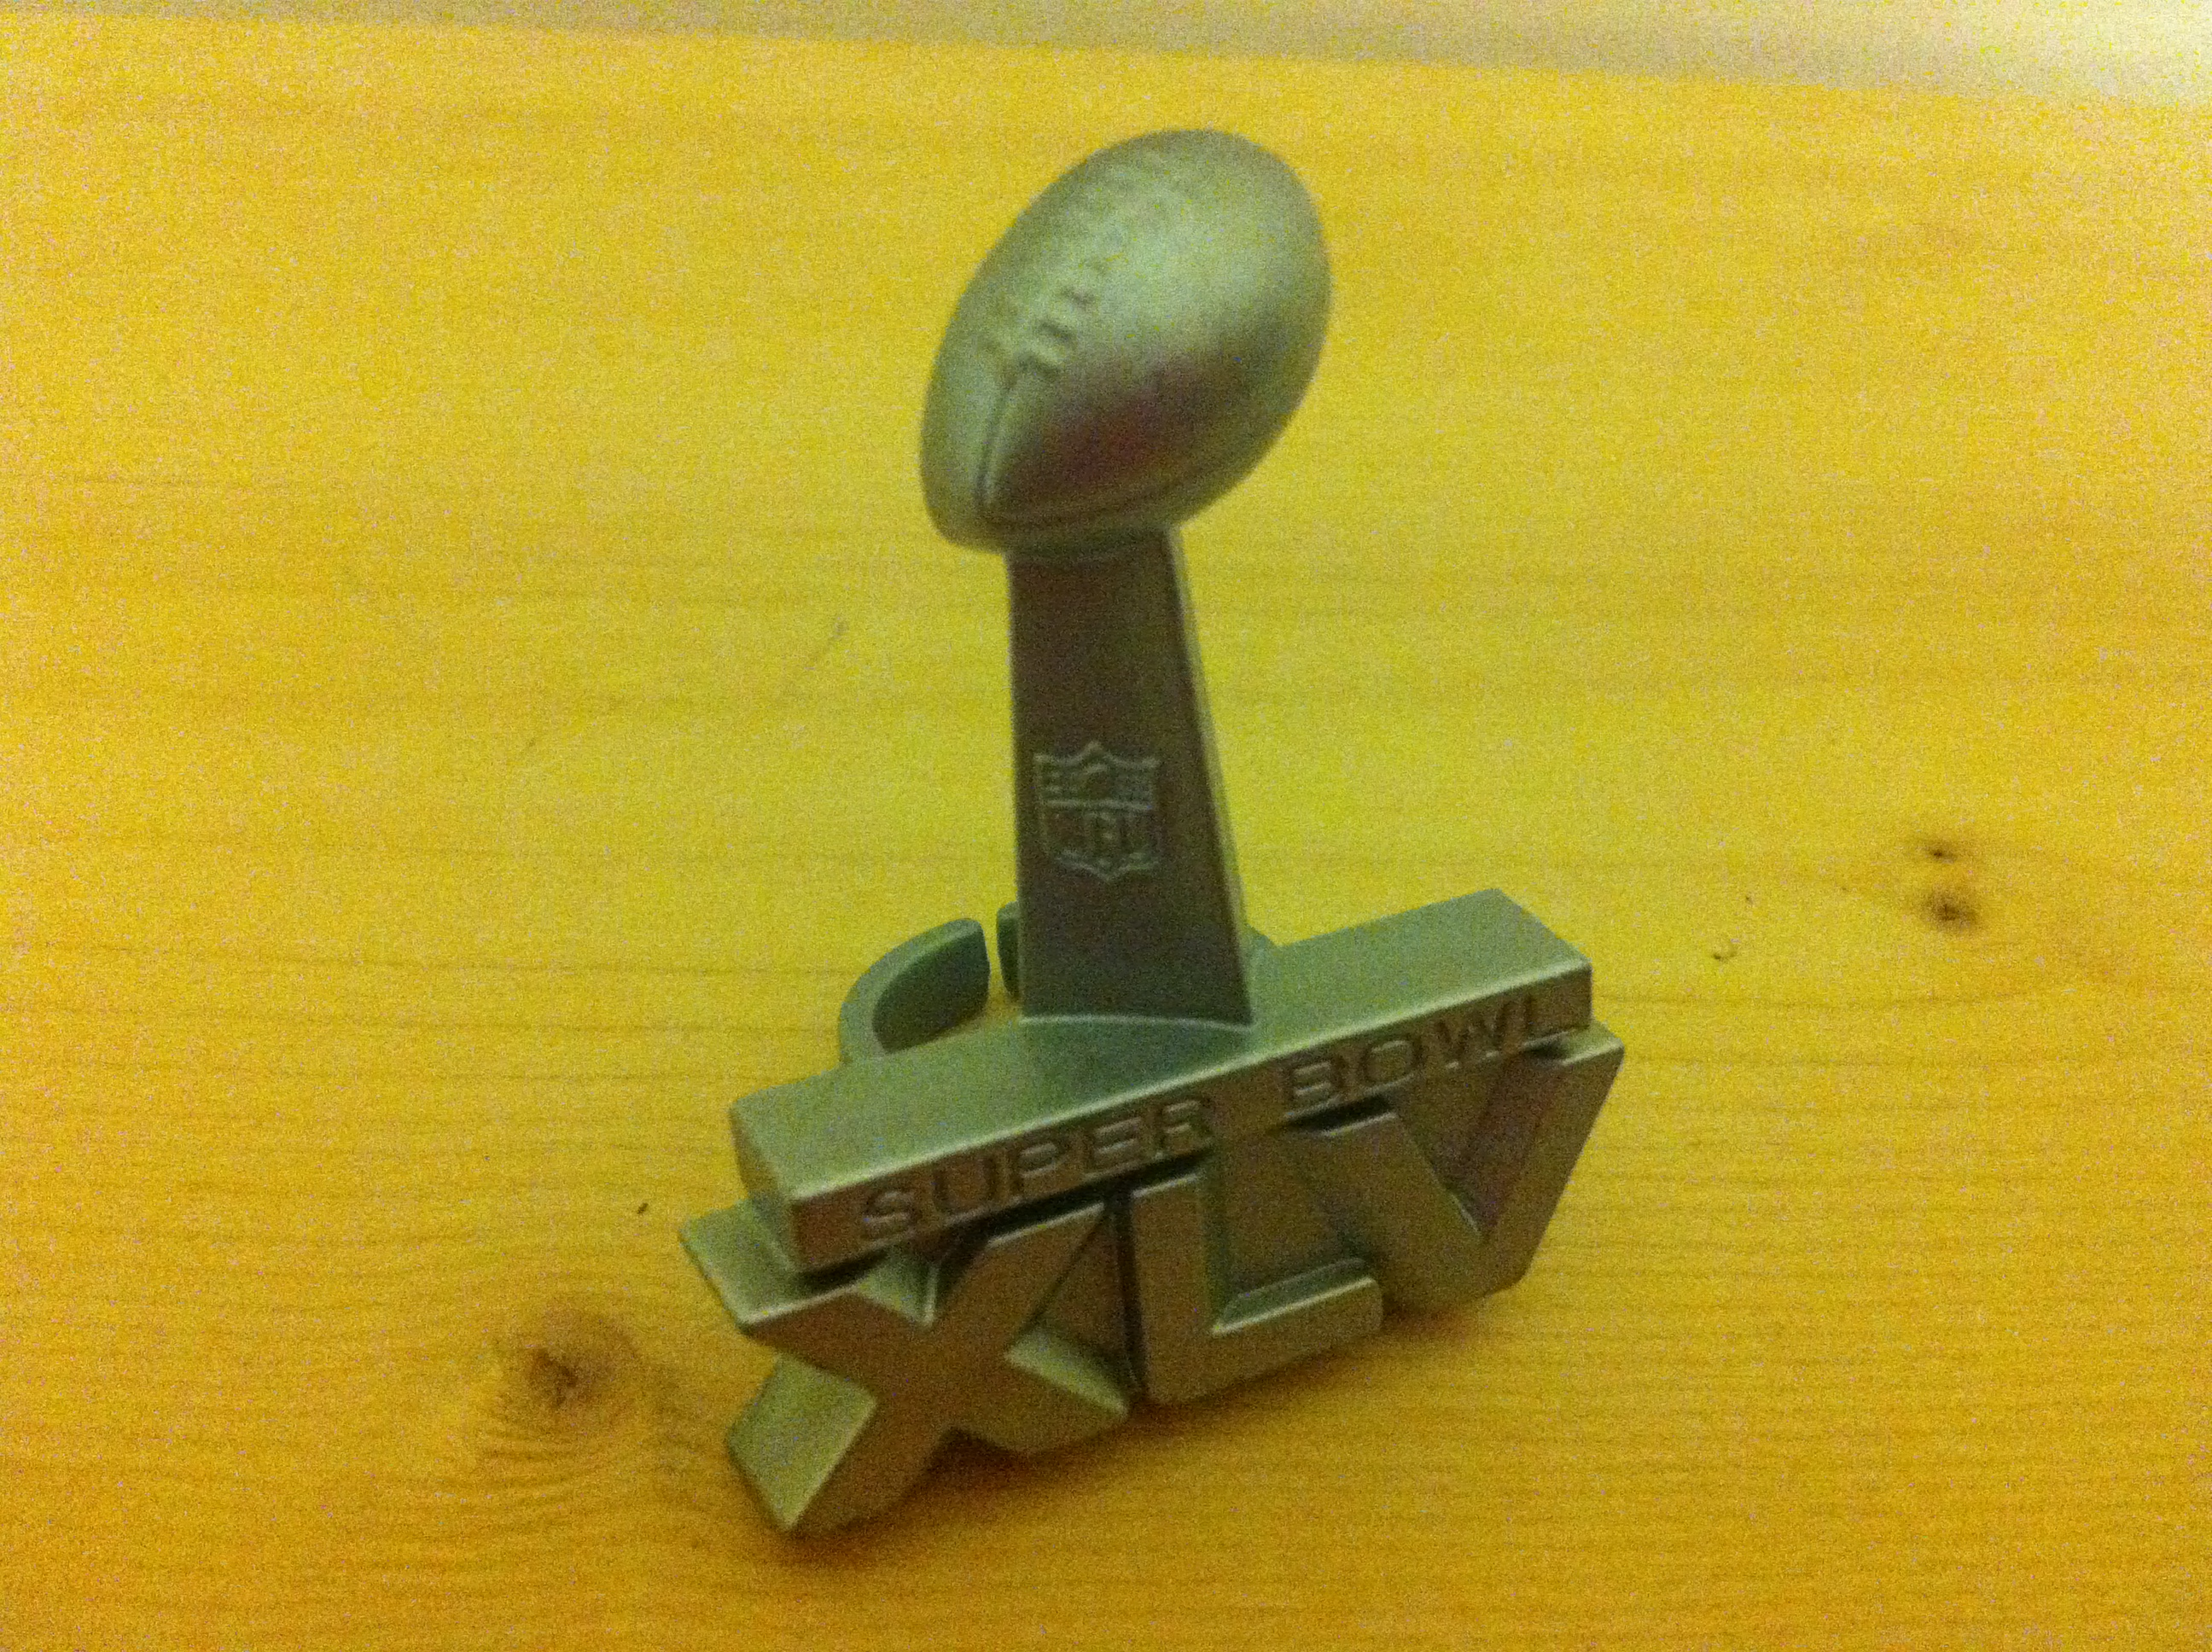
\includegraphics[width=.9\linewidth]{./pic/IMG_0371.JPG}
\end{center}

\section{我和表哥(3)}
\label{sec:org1fb5226}

\begin{center}
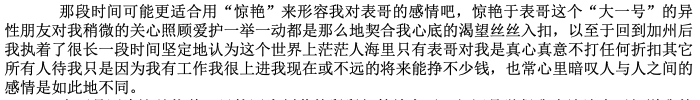
\includegraphics[width=.9\linewidth]{./pic/p1p49-0.png}
\end{center}  

那个停车场,我对表哥表白后,表哥的回答却是“我十年之内都不会结婚!”表哥顾左右而言他,而我却在那一刻瞬间“白发”,低头眼泪一下子就涌了出来。如果说我自己的感情生在一段偏僻处,那表哥的感情也一定很清奇。既有今日,何必当初?等我平复了情绪,毕竟我们之间亲密,转过抬头看向表哥,破涕为笑地说,“好丢人啊,现在我姐姐她们都知道了,回头她们又要取笑我了!”表哥见我不哭了,就追问起上次走时是怎么回事。

那个同表哥求温暖、求抱抱的告别在我这里已然成为一场浩劫,表哥却不承认,那我也不承认,就按高中那时压垮我的算命先生的话来答表哥。

\begin{center}
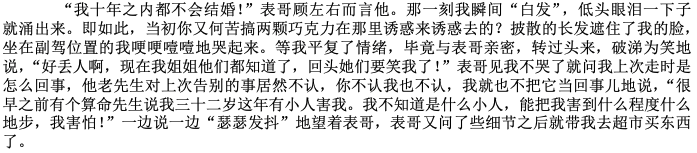
\includegraphics[width=.9\linewidth]{./pic/p1p50-0.png}
\end{center}  

刚刚向表哥表白被拒的尴尬很快被我忘掉,表哥带我去超市买东西。进门时有工作人员正在给进场购物的消费者发送礼物,表哥领到一件,表哥就转手送给了我,是一枚戒指!

\begin{center}
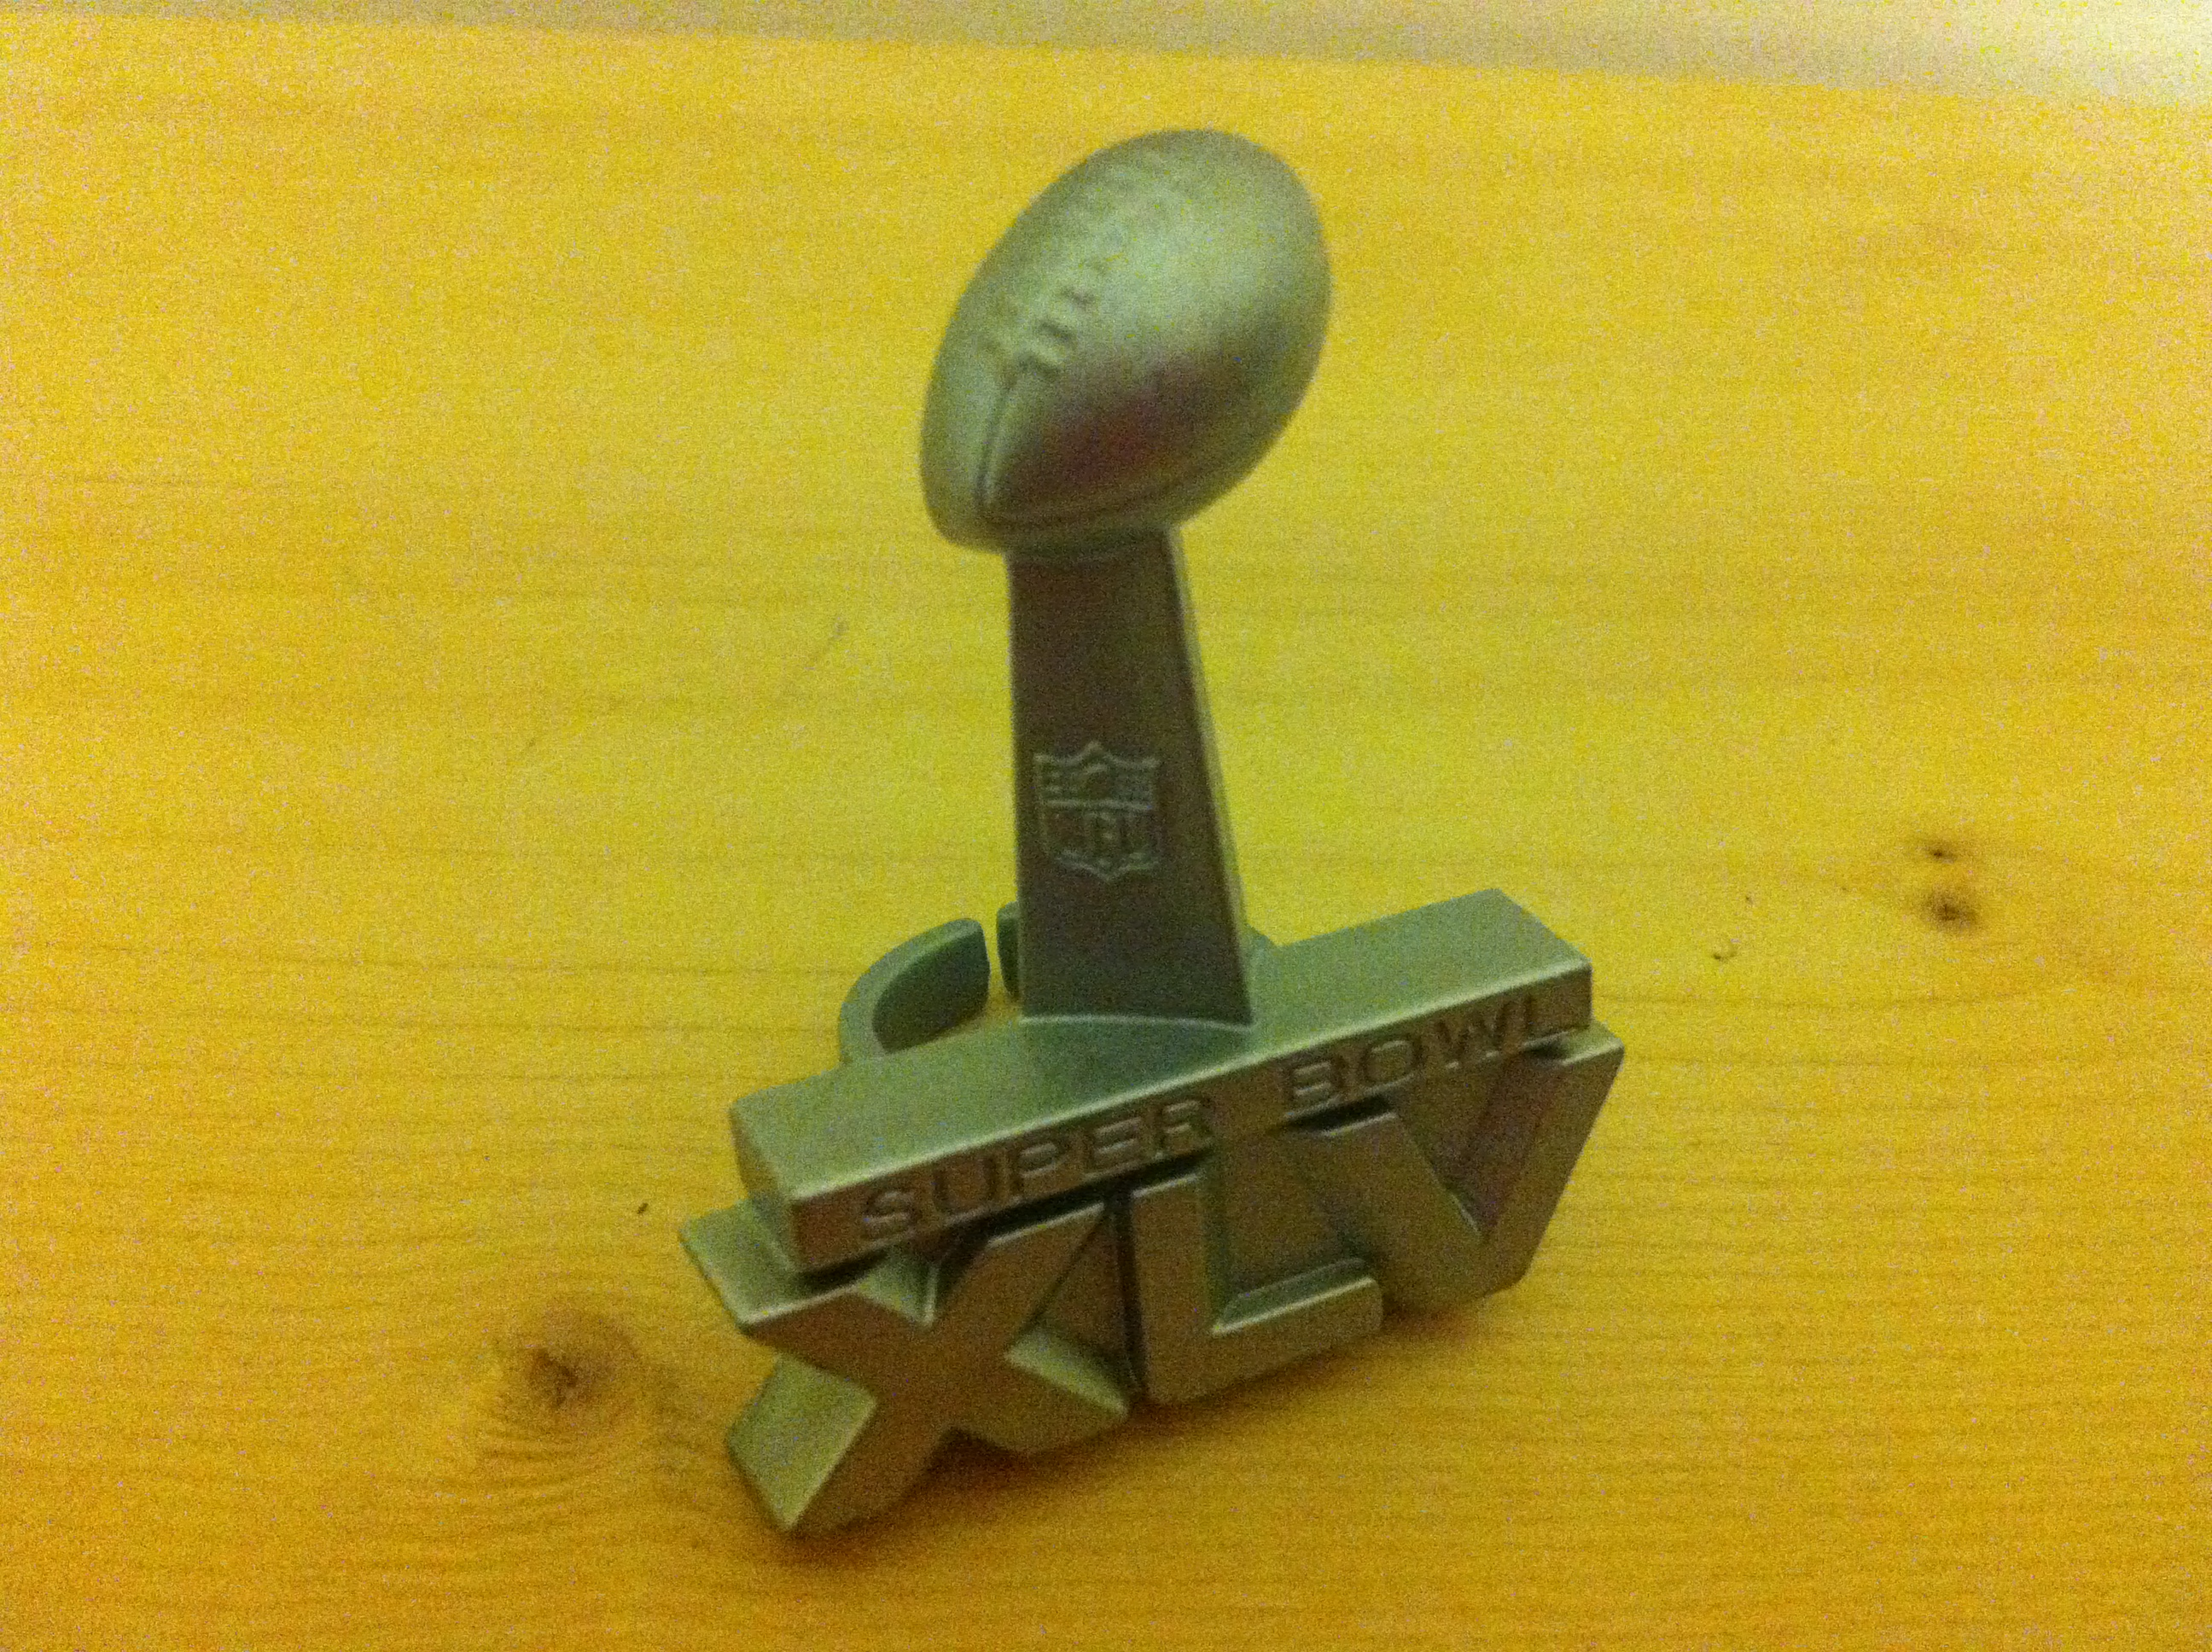
\includegraphics[width=.9\linewidth]{./pic/IMG_0371.JPG}
\end{center}

我们推着一辆购物车在各走道里穿行。即便有时我自己推车,表哥也会时不时地伸出一支胳膊来援助我。我们像极了情侣,亲密快乐!我们还是很引人侧目,不过谁有精力、顾得上去理会那么多呢?

\begin{center}
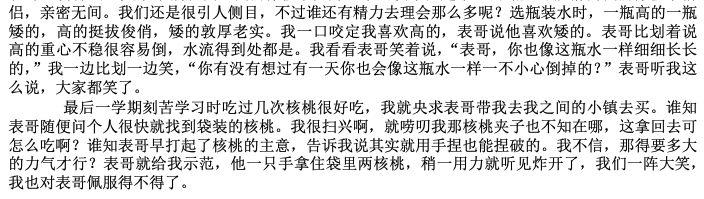
\includegraphics[width=.9\linewidth]{./pic/p1p50-1.png}
\end{center}  

与表哥在车时的什么时候,表哥有说过一句,“其实我也可以带你去office”。那天我头很痛,听到表哥这句话,我强力思索一番,就对表哥说,“表哥,我不信,你今天说过的所有的话我都不信。”

\begin{center}
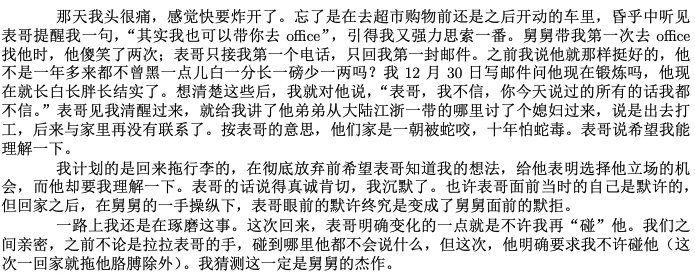
\includegraphics[width=.9\linewidth]{./pic/p1p50-2.png}
\end{center}  

这次回来,我是计划好需要向表哥表白,让他知晓我的立场;因为之前电话里舅舅过分的话语(我打给舅舅的电话里,舅舅说过性格不好,嫁不出去,没人要,并说我是骗子),我也是回来拖行李,如果表哥拒绝我,我应该需要与表哥有个了断,我也该把我的行李都拖回加州。

购物时表哥车里的话我记在心里,但在我长途开车睡眠不足头快裂开的情况下,我当时没能立即反应过来,就是如果我真努力去理解一下他们那个家庭,我就当那次是回去了解一下家里的情况,就不要再在那一次将行李拖走,给双方留下一点儿缓和的时间。但当时的我反应不过来,表哥的话得需要我回到加州后补充睡眠休息好后好好体会才能消化得了。

舅舅家的四方桌已经折掉了,添置了新红木样式陀圆形轮廓大餐桌。像是得了强迫症一样,我掏出支票本,给舅舅写一张\$4000的支票以还清上统计硕士期间从舅舅家借出的债务。至此,我到家之前原计划的回家任务才算是基本完成了。

如果说表哥的话我尚且没有消化的时间一时消化不了反应不过来,等到舅舅家后等我搬完行李进自己的车,写完还债的支票,接下来舅舅的话说像一个武林高手拿着利箭,剥我的皮、削我的肉,残忍暴烈到让我惊悸不已!

\begin{center}
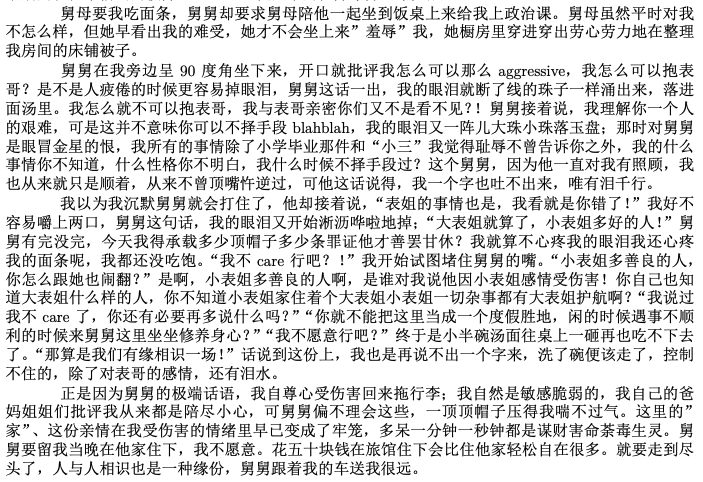
\includegraphics[width=.9\linewidth]{./pic/p1p51.png}
\end{center}  

这次写时,我突然想起来,2008年舅舅建议暑假舅舅会送我去加州硅谷小表姐Cindy Wang处,他要教会我如何用非专业相关的工作攒钱生存,并得以成行。在舅舅与我轮流驾车开往硅谷的路上,我们讨论过在小城市还是大城市生活比较好这个话题。舅舅喜欢小城市的安宁、交通方便等。我则小半生的经历都是在实现着从祖藉家乡往外走,从襄阳到武汉、到北京,往远处走到美国乡村,再到这次舅舅带我来美国硅谷。我的成长经历把自己锻炼成一个比较有进取心的人,我还是比较向往小表姐那样能够在大城市扎下根来的生活。舅舅陪驾护送我来硅谷,我想舅舅是能够体会我心底对大城市那份实实在在的向往。

舅母提起过表哥家附近就有一个什么样的类似工厂一样的科技公司,舅母说表哥毕业后能在那里上班就好。显然,在表哥这样的年龄,表哥可能不是很愿意搬去大城市或是在这样的年龄还去大城市打拼。

除了舅母早已帮我摆出来的这个表哥与我将来生活地点选择的不同之外,经历了10年12月那个周一那场万劫不复的告别,我知道我今生应该就是跟定表哥了,但那也并不排除我在现实面前、在当前的物质基础下、在对表哥的家庭没有足够信任的前提下、在感情尚处在萌芽状态、作出自己本能的、适当的、又或者垂死地挣扎。

在当年那些年我幼稚的思维里,甚至曾经有过,2001年我写信给你,你都没有帮忙把我早一点儿带出来读书,让我误了这么多年,我凭什么要作你们家的儿媳妇?这样的想法。 

\begin{center}
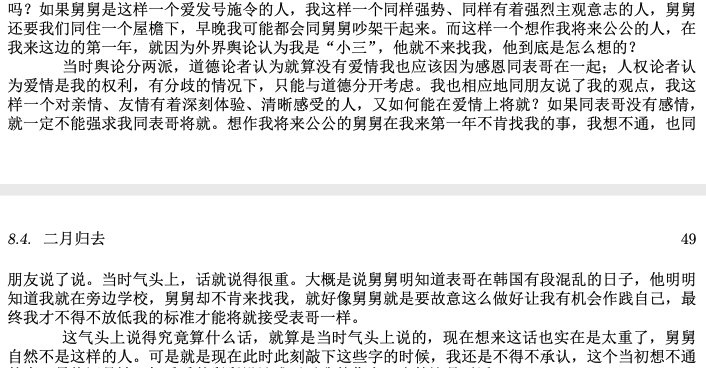
\includegraphics[width=.9\linewidth]{./pic/p1p48.png}
\end{center}  

\section{我和表哥(4)}
\label{sec:orga7a4296}

来美留学早年,校园生活里那些年的我,生活中常常充斥着各种各样的不知道什么原因造成的逆势,但那时的我对这些舆论是不敏感、没有意识也不曾去深想过,究竟是什么原因造成了那些诸多的逆势。 

正如2010年一二月那天早晨,当表哥在家里等我,以便我南下加州前能再互相见一面,我心里燃起过点点火花,来到加州便在大表姐Sherry Wang面前经常提起表哥,大表姐总是阻拦我,劝我在我现在人所在的地方,加州硅谷找男朋友。

\begin{center}
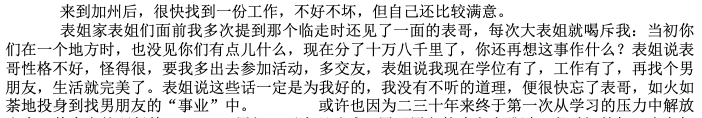
\includegraphics[width=.9\linewidth]{./pic/p1p40.png}
\end{center}

2010年12月,与表哥的那场矿世告别,我心里清楚地知道,我喜欢这个人,我这辈子应该就跟定表哥了。

\begin{center}
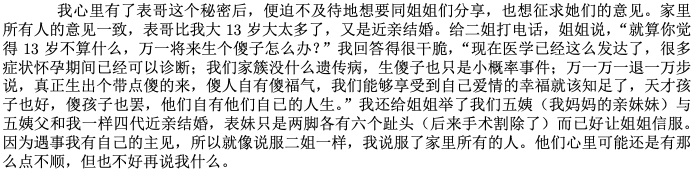
\includegraphics[width=.9\linewidth]{./pic/p1p44.png}
\end{center}

可世俗社会里,对表哥的家庭的认识与理解、他们家庭的生存现状、表哥将来的工作单位和生活所在地,都与我内心深处尚未放弃的对大城市的向往是不符合的。

于是,涉世不深、感觉个性尚未定性的我,面对这个世俗社会,在当前的物质基础下、在对表哥的家庭没有足够理解与信任的前提下、在表哥与我的感情尚处在萌芽状态(虽然内心里早已是台风过境般坚定地认定了对方)早期状态、我作出了自己最本能的、又或者自认为最彻底地挣扎。

\begin{center}
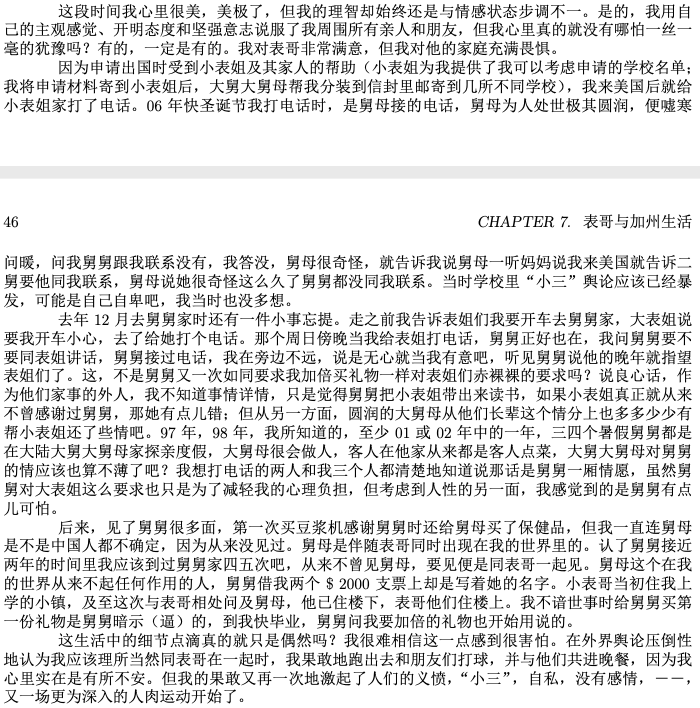
\includegraphics[width=.9\linewidth]{./pic/p1p46.png}
\end{center}

就像我前面曾所提及到的,公开场合,我的确清楚地表达到,我这样一个对亲情、友情有着深刻体验、清晰感受的人,又如何能在爱情上将就?如果同表哥没有感情,就一定不能强求我同表哥将就。

亲爱的读者,在与表哥的那场旷世告别,在我内心清楚地知道,我这辈子应该就跟定表哥了,可在我最原始最为本能的防卫式自我保护面前,上面的立场(真心表达我对自己爱情的选择立场),虽然它一定不是我本心(在真正爱上表哥后,还对外抛出这样的话,则是我当初本能地反抗自我保护的本能,对外假装成我还不爱表哥,不是我真心,却是我自我保护的本能),但它不就该是最本能与最为彻底的反抗了吗?可时间会告诉我们,在这份感情的自我保护本能反抗而选择果敢出行,故意与硅谷当地男生有户外活动交集,与同表哥的真爱里,哪个是真,哪个是假,一如时间将证明,舅舅表哥、与王夏华王秋勤两组亲情里,谁对我真,谁对我假!

在2010年、2011年那短暂的被物质所牵扯、被大表姐Sherry Wang用各种现实洗脑,猪油蒙了心,那个时候我的立场、我所摆出的公允证据其实还需要时间沧河的检验。待十年过去,此时再来那一番评价,就像今春加州的三月冰雹、往年的六月飞雪,那时评价得舅舅比窦娥还冤。对大表姐Sherry Wang和Cindy Wang及其父母一家人,我会在接下来的某一两篇专题叙述。

这里,从当时的纪录可以明显地看出,三大中文网站的炒作如日中天、纷纷扰扰,但一如早年留学生活的我,那早年工作经历的2010-2012年,尤其是2010、2011年,我的情商不在线不上线,根本从来就不曾搞清楚过三大中文网站的炒作与我的现实生活、与我的工作有什么关系。

\begin{center}
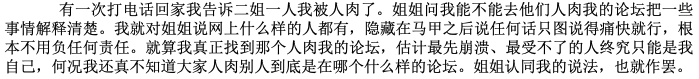
\includegraphics[width=.9\linewidth]{./pic/p1p51-2.png}
\end{center}

我也从来不曾作出过任何的回应,直到2011年11月被迫站出来写自已的自传以求澄清自己。但之后的很长一段时间内我仍搞不清楚三大如日中天的炒作与我的工作生活有什么联系,直到2012年春天统计实习的最后一份工作,最是后话。 

\section{我和表哥(5)-- 2011年四月与五月底回家}
\label{sec:orgad788a4}

\begin{center}
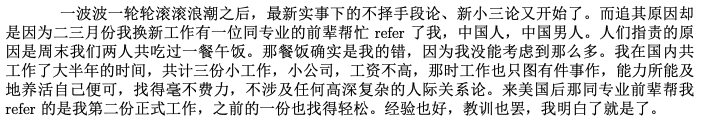
\includegraphics[width=.9\linewidth]{./pic/p1p52.png}
\end{center}

那时的我在加州工作,周围的朋友圈也还是有一个华人男生,但在假装的喜欢面前,我骗得了别人,骗不了自己的心。 

\begin{center}
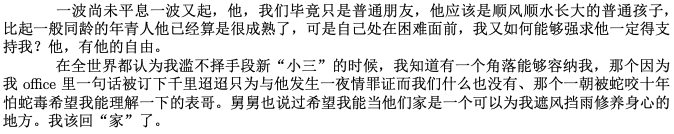
\includegraphics[width=.9\linewidth]{./pic/p1p52-2.png}
\end{center}

2011年四月回去,表哥还是一心一意、全心全意地待我。当年那个没有情商、一心等待索要口头承诺的妹妹呀,现在回去看都替当年的自己着急。 

\begin{center}
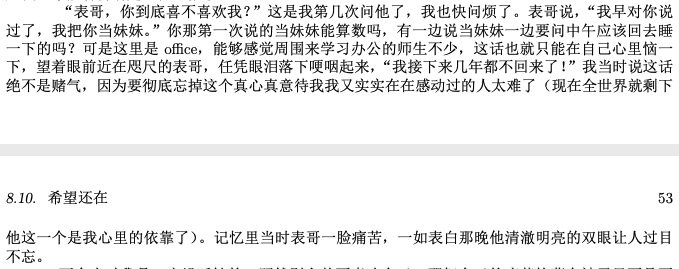
\includegraphics[width=.9\linewidth]{./pic/p1p52-3.png}
\end{center}

那天晚上回到家后的柔情。 

\begin{center}
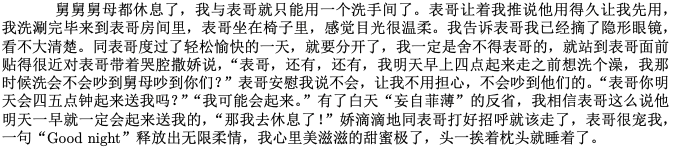
\includegraphics[width=.9\linewidth]{./pic/p1p54.png}
\end{center}

这次回去再读这一段的时候不免奇怪,即然自己已然摘了隐形眼镜都能够感觉到表哥的目光温柔,为什么当时的自己就没有任何进一步的行动呢?你不是早先也期待过一个拥抱一个吻的吗?为什么当初的自己就不曾再努力争取一下呢?后来想想,一方面可能是那时的自己笨,恋爱经验不够,情商不够,原本就不知道自己当时应该怎么做(虽然当时的自己仍记得2009年春天当我抱着打印出来的当时男友的生肖星座去找舅舅时舅舅说过让我顺着甚至于发生点儿什么);但另一方面, \textbf{潜意识里} ,与表哥的那场告别已然让我万劫不复从前,今生都将永远地与表哥捆绑在了一起,我意识到了亲密行为的威力与可怕(你今天也终于意识到这一点了哦?!那为什么二月份走时舅舅指出、批评这一点儿的时候,你就一点儿也听不进去呢?要等到什么时候你才能够比较坦然地接受别人的指正与批评呢?),在亲密行为面前我开始变得不够勇敢、有些犹豫。在我自己还没有完全准备好的状态下,再多的亲密行为对当时的我来说可能显得稍微pushy吧.

回到加州的路上,我一路愤愤不平,表哥这次为什么没有起床送我呢?

\begin{center}
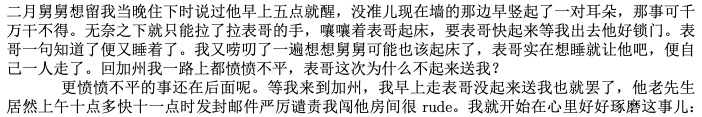
\includegraphics[width=.9\linewidth]{./pic/p1p54-2.png}
\end{center}

回到加州后,我更是收到了表哥的邮件只把我当妹妹!

\begin{center}
\includegraphics[width=.9\linewidth]{./pic/p1p55.png}
\end{center}

从与表哥谈恋爱后,舅舅就被我本能地打回到退居二线。

\begin{center}
\includegraphics[width=.9\linewidth]{./pic/p1p55-2.png}
\end{center}

五月底的长假,我打算回表哥那里。虽然电话里告诉舅舅的时候舅舅说他不欢迎,但为了表哥,我还是早早地计划并同表哥更新行程安排(从后来发生的事情来看,显然当年幼稚的我没能想清楚舅舅的不欢迎意味着什么。舅舅与表哥之间,我的意识那时像是还很模糊)。表哥默许,五月底那个星期三的下午,我就早早地兴冲冲地出发回表哥家了。

我一如既往地先到表哥的办室里找到表哥,再央求表哥把我带回家,回到家我可以洗澡把自己打扫干净,表哥也让我品尝了他知道我要回来,他自己亲手做的蛋糕。家里面表哥浴室的外层装饰性浴帘和橱房餐厅里的窗帘由以前的白色换成了庄重典雅的大红深红色。等表哥带我回到他的办公室,是周四,表哥的老板与同博士生同老板的同门师弟也在。我们就开始聊天。

表哥的老板请我们品喝他家乡的碧螺春,泡水后绿油油的,清香沁脾。表哥不带我出去吃米饭、不带我吃面条,说过吃pizza吧,表哥又把我们的午餐推给了他的老板。表哥的老板带我和他的那个博士生一起出去吃pizza。路上表哥的老板提醒我对我说,小姑娘不要读书读傻了,你要替你自己考虑。老板说看你表哥现在什么样子,你要想想你这么多年来读书是为了什么,是为了跟这样一个人在这样一个鸟不下蛋(鸟不拉屎)的地方过苦日子吗?老板说,小姑娘儿们喜欢听歌,花两三百块钱买副耳机、听听歌看看电影什么的都太正常了。几十年、二三十年寒窗苦读为的是什么,不就是为了工作后能过上好日子吗?表哥的老板劝我,以后最好就不要再回这个地方了。

回到办公室后,老板把那盒我们外面吃剩的pizza递给了表哥,他应该还没有吃中饭。看着表哥接过披萨盒的样子,我很心酸,心想着,如果我听了你老板的话,真的逃跑成为了这场爱情里的逃兵,表哥你今后的人生会过成什么样子?

\begin{center}
\includegraphics[width=.9\linewidth]{./pic/p1p57.png}
\end{center}

那天,我同表哥说着我们晚上早点儿回家吃饭,晚上想吃点儿米饭,想傍晚在家好好休息一会儿。可是回到家,看到舅舅堆在家门口的礼物袋,敏感、没有安全感的我就又一次地傻了眼,又一次地从那个家逃跑了!

\begin{center}
\includegraphics[width=.9\linewidth]{./pic/p1p58.png}
\end{center}

\section{Career Space Sexual Interference}
\label{sec:org7e2d337}
这个是2012年10月底我已然回到学校读计算机硕士时,被三大文网站拿出来炒作与黑我,我被迫写下关于2011年3月至5月底那份统计工作的澄清。

在2011年那场与表哥的相遇以及纠葛、以及后来表哥的邮件、情感陪伴我度过2012年OPT实习期间那份统计专业的最后一份工作时,感觉在2012年慢慢才情商上线。之前三大中文网站的炒作,我根本就搞不懂是怎么回事,甚至于连2012年春那份统计工作也都还有些模模糊糊。

\begin{center}
\includegraphics[width=.9\linewidth]{./pic/p1p143.png}
\end{center}

\begin{center}
\includegraphics[width=.9\linewidth]{./pic/p1p144.png}
\end{center}

\section{我和表哥(6)}
\label{sec:orgfffe2d2}
2011年3月,因为统计第二份工作的关系,我3月从南湾San Jose搬至Oakland中国城住了四个月左右,离上班的地方会近些。五月底从表哥家回来那次,丢掉了那份统计工作,经历了大概半个月的调整,我打算搬回南湾原房东处去住。

\begin{center}
\includegraphics[width=.9\linewidth]{./pic/p1p61.png}
\end{center}

10年12月与表哥的那场告别,让我清楚地知道我的归属。可出于本能地保护自己,我装作了对南湾当地一个活动中有交集的男生有好感,但我装作喜欢别人,最终也只能是骗得了别人,骗不了自己!

\begin{center}
\includegraphics[width=.9\linewidth]{./pic/p1p110-2.png}
\end{center}

\begin{center}
\includegraphics[width=.9\linewidth]{./pic/p1p61-2.png}
\end{center}

五月底那份工作丢掉后,我找工作找了一两个月都不太顺利,很多朋友都怂恿我去找表哥,嫁给表哥就什么都好了。我也就自然而然地想起表哥来。

\begin{center}
\includegraphics[width=.9\linewidth]{./pic/p1p62.png}
\end{center}

在我这里,从10年12月那个周一的矿世告别,我心里早已认定我这辈子是会跟定表哥的,这一点在我这里是今后五年、十年二十年甚至于后半生的总方向,绝不动摇。至于说我清醒地意识到这一点后最开始的本能反抗、与舅舅家因为不理解不足够信任而产生的纷争其实也都只是周边和副效应,又或者说是清楚地认识到那一点儿之后我在世俗社会里如同表哥老板所秉持的一般而进行的垂死挣扎,只要大家有机会能够坐下来好好谈,那些都是可以很容易解决的小问题,不碍大事、不碍大的决定。 

或许在我一遍遍问及表哥什么时候毕业(虽然舅舅总是说表哥是天才,国际上发表了60多篇文章,想什么时候毕业就什么时候毕业),或许表哥认识到我心目中的大城市梦对我有多重要,或许表哥想要陪伴我走一程,不知道从什么时候起,表哥的LinkedIn的网页已经建立起来,他的联系人出由我最开始注意到的4个变为6个。

\begin{center}
\includegraphics[width=.9\linewidth]{./pic/p1p63-1.png}
\end{center}

在后来读计算机专业第一个学期我什么也不懂老师一布置作业我就怕的岁月里,在后来生活中所经历的各种选择与变数面前,表哥的鼓励都成为我后来成长过程中最长情的陪伴,一直停留在我身边不曾走远,这是后话。

我是一个有闪婚情节的人,觉得两个人只要相互喜欢就可以结婚了。

\begin{center}
\includegraphics[width=.9\linewidth]{./pic/p1p63-2.png}
\end{center}

我对表哥家舅舅的恐惧与不理解,会成为障碍吗?不会。 

\begin{center}
\includegraphics[width=.9\linewidth]{./pic/p1p63-3.png}
\end{center}

我坐在门口等啊等,望啊望,等待邮差的到来,但我等来的却是两封拒信。 

\begin{center}
\includegraphics[width=.9\linewidth]{./pic/p1p64.png}
\end{center}

\section{我和表哥(7)}
\label{sec:org1d0ea66}

表哥的邮件像是小论文,有论点论据论证,却被我这颗不太灵光的脑袋直接读成了抒情散文,读到浮想联篇,意绵绵邮件生香。

\begin{center}
\includegraphics[width=.9\linewidth]{./pic/p1p64-3.png}
\end{center}

表哥邮件的信息量过大,我一时半会儿是想不明白的。可接下来不到一个小时,舅舅发送过来的邮件就直接送我go to hell! 原表哥邮件的内容便被当时的我华丽丽地忽视了?!

\begin{center}
\includegraphics[width=.9\linewidth]{./pic/p1p64-4.png}
\end{center}

为什么读到舅舅的警告邮件,我会如此地愤怒!回想我和舅舅所建立的信任又是怎样的呢?

\begin{center}
\includegraphics[width=.9\linewidth]{./pic/p1p65.png}
\end{center}

回想一下,我喜欢表哥的大致过程应该是这个样子的。

\begin{center}
\includegraphics[width=.9\linewidth]{./pic/p1p66.png}
\end{center}

我为什么会愤怒?舅舅对我施加了冷暴力!

\begin{center}
\includegraphics[width=.9\linewidth]{./pic/p1p66-2.png}
\end{center}

内伤是什么?内伤会磨折人的灵魂。

\begin{center}
\includegraphics[width=.9\linewidth]{./pic/p1p66-3.png}
\end{center}

我不愿意再饱受摧残,为防止内伤的再次形成,我一定要回去闹一场!

\begin{center}
\includegraphics[width=.9\linewidth]{./pic/p1p66-4.png}
\end{center}

时光荏芮、白驹过隙,转眼已是又十年。当十天前(3、13、14、2021)的周末我第一次去回读自己十年前写下的文字,当我清楚地意识到十年过去,我原本拥有的很多珍贵记忆都已然从我的脑海中消失,当我清晰地读出当年自己个性中的自卑、敏感、脆弱与依赖,我终于明白舅舅并不是当年我所认为的十岁便踏足社会炼就的冷血,而是一如他曾经对我说过的“要受过什么苦受过多少磨乱创伤才会使人变成这样”,他对别人的苦痛体察入微。

\begin{center}
\includegraphics[width=.9\linewidth]{./pic/p1p122.png}
\end{center}

舅舅和表哥怕我这个迷途走丢的孩子找不到回家的路,表哥成为了我的定海神灯,而他们一路标记,帮助我记忆不致遗忘。表哥和舅舅,都是人类灵魂的工程师,而我们,从来都是同一国的。那日读到此,禁不住眼泪扑涑而下,感动不已!此是后话。 

\section{我与表哥(8) -- 与舅舅冷暴力的对决}
\label{sec:orgfecb7cc}

我的亲表哥(我妈妈亲哥哥的儿子)在我成长过程中给我打下了挥之不去的深深烙印。正如我的亲表哥血液里流淌有大姐夫的血液,我的个性里也还有太多那些年成长过程中亲表哥给我留下的阴影,叛逆、固执倔强等等。

\begin{center}
\includegraphics[width=.9\linewidth]{./pic/p1p67-2.png}
\end{center}

来到表哥的办公楼,我先来到了表哥的办公室。表哥不在,门没锁,我就进去爬表哥床上先休息一会儿。 

\begin{center}
\includegraphics[width=.9\linewidth]{./pic/p1p67-3.png}
\end{center}

我去用表哥办公室外面的洗手间,我始终没有动过表哥办公室的门,但等我从洗手间回来,表哥办公定的门已民经锁上了,我进不去,手机也锁在了里面。 

\begin{center}
\includegraphics[width=.9\linewidth]{./pic/p1p67-4.png}
\end{center}

表哥家我去过好多次了,但路我总不记得。表哥的办公室离表哥家也很远,骑自行车都需要二三十分钟半个小时左右,我没有车钥匙只能走路,加上极度疲乏下,不熟悉路又绕了弯,一两个小时才总算找到了表哥的家。 

\begin{center}
\includegraphics[width=.9\linewidth]{./pic/p1p67-5.png}
\end{center}

进屋后我就用了一下表哥的洗手间,洗手间里不争气的眼泪忍不住就掉了下来,太累太辛苦了。 擦干眼泪,跑出去敲表哥的门,里面没人应。推开门,见表哥穿着背心短裤平躺在床上休息,待我推开门,抬了抬头看了看我。 

\begin{center}
\includegraphics[width=.9\linewidth]{./pic/p1p67-6.png}
\end{center}

\begin{center}
\includegraphics[width=.9\linewidth]{./pic/p1p68.png}
\end{center}

我与舅舅、表哥一家人的缘份应该到此也就结束了吧,当时我想。 

\section{我和表哥(9)}
\label{sec:orge657d23}

表哥的电脑里,我喜欢的那些小动物们,表哥都帮我收藏得好好的(这次我回去读到表哥曾经给我讲过的一个园子里斑马和孔雀的故事,不是这次回去读重新忆起,我可能就永远把那个表哥拍他俩儿时的故事情节给忘掉了。希望改天表哥再给我看一看、为我再讲一遍那些小动物们的故事)

\begin{center}
\includegraphics[width=.9\linewidth]{./pic/p1p67-10.png}
\end{center}

表哥的那条我常掏口袋的裤子,我一点儿也想不起来了,是什么颜色什么款式的?隐约中犹记得有一次从表哥裤口袋掏出一个小本儿,表哥说是舅舅给的,表哥当时给我解释过那个本他是用来做什么的,以及舅舅给表哥时对表哥讲过什么样的话,表哥当时给我详细地讲过,但这些年过去,除了我仍记得从表哥口袋里掏出过一个小本儿,和表哥告诉我那是舅舅给他的之外,其它的情节,现在的我一点儿也回忆不起来了。还包括后来13年春天表哥从洗手间出来,在表哥房间我抓他的衣服时,表哥下面穿着短裤,上面里面是很件很合身的白色T恤,可是外面套着的那件线衫后来被我抓脱了的线衫,我也是一点儿都想不起来了。希望表哥把这两件衣服收藏好(把那本小本儿也帮我收藏好,我现在也想不起来它长什么样子的了),等我回去,重新穿给我看(大哭!)

舅舅告诉警官的他的生日37年,与记忆中某次同舅舅聊天时所得到的36年重阳节(阳历9月24日)不符合,但这个细节并不重要,记错弄错都无关大事。

\begin{center}
\includegraphics[width=.9\linewidth]{./pic/p1p67-9.png}
\end{center}

读到这里,我忍不住笑了,当年的小丫头片子呀!早年间不懂感情、心智不够成熟、情商不上线不够用的我,因为想下午早点儿回来洗澡回来得早了点儿被舅母提醒炉子还有大小姐脾气时好时不好的,我都没搞明白人家是在说什么,预防针打下了,小人儿也扎上了,唉唉!

\begin{center}
\includegraphics[width=.9\linewidth]{./pic/p1p68-3.png}
\end{center}

这是那时我收到舅舅邮件愤愤不平回去找舅舅时,极度残忍冷血的舅舅第一次对我说:他可以拿枪一枪打死我,不用负任何法律责任!当我听舅舅说他要拿枪一枪打死我的时候,我就热血直往头上涌,感觉头快要炸开,痛苦之至。要怎样冷酷绝决的人才会想要把自已家乡的亲人用一杆枪、一发子弹了结而问心无愧?

后来舅舅的这句挑战我极限的名言,又被他变着方儿的用过一次,所兴极致名言最终还是发挥了它应该起到的作用,这是后话,暂且不表。 

\begin{center}
\includegraphics[width=.9\linewidth]{./pic/p1p68-2.png}
\end{center}

在对警察的陈述里,舅舅说我是骗子,舅舅说他离开家乡多年,不知道他的家乡有我这么一个亲戚,舅舅说我是表哥的first cousin,我就再也听不下去了。因为舅舅、我和表哥谁都知道,我们并不是first cousin. 舅舅的爷爷与我妈妈的爷爷是同一个人,哪里是什么first cousin呢?Cindy Wang王秋勤和Sherry Wang王夏华才是表哥的first cousin好吧?!

2010年12月我热恋表哥时,就经常打电话到舅舅那里,同舅舅聊天。

\begin{center}
\includegraphics[width=.9\linewidth]{./pic/p1p45-2.png}
\end{center}

第一次的电话里,我仔细地问过舅舅口中,我与表哥的亲缘关系,舅舅给出的是与我妈妈给出的相同的答案,我们并不是first cousin呀!我当时还问过舅舅的态度,舅舅说他既不支持,也不反对。

\begin{center}
\includegraphics[width=.9\linewidth]{./pic/p1p120.png}
\end{center}

后来,2012年5月,当我知道我即将失去统计OPT期间最后一份工作,即将失去作为狮子座女孩的尊严保护伞时,我在工作结束前回去找过舅舅。我仔细问过舅舅当初他为什么要那么说,舅舅说,他量我怎么地表哥也不可能喜欢我!

\section{我和表哥(10) —— 表哥的拒信}
\label{sec:orgeaac3d5}

\begin{center}
\includegraphics[width=.9\linewidth]{./pic/p1p64.png}
\end{center}

表哥说我前三次去找表哥,表哥每次都给了我他的答案。

10年12月份那场惊心动魄的告别里,我一句话还没有说完,表哥“我把你当妹妹!”的话就已然打断了我。

\begin{center}
\includegraphics[width=.9\linewidth]{./pic/p1p43.png}
\end{center}

那年(2011年)二月,激情热恋中的小丫头说服了家里所有的亲人,以为自己当时的状态都可以跟表哥结婚了,跑回去向表哥表白,表哥说他“我十年之内都不会结婚”;

\begin{center}
\includegraphics[width=.9\linewidth]{./pic/p1p50-3.png}
\end{center}

那年四月,表哥的办公室里,我问表哥他到底喜不喜欢我,表哥说他把我当妹妹!

\begin{center}
\includegraphics[width=.9\linewidth]{./pic/p1p52-3.png}
\end{center}

表哥说过的话,他拿我当妹妹,我信不信,二月份的时候我也已经想过一次了:当场反问过表哥:“表哥,我不信,你今天说过的所有的话我都不信。”

\begin{center}
\includegraphics[width=.9\linewidth]{./pic/p1p50-4.png}
\end{center}

表哥喜不喜欢我,四月份那次我都已经想得很清楚了:表哥一定是喜欢我的!

\begin{center}
\includegraphics[width=.9\linewidth]{./pic/p1p53.png}
\end{center}

表哥一定是喜欢我的!表哥只是说不出来,可能天秤座的舅舅尘世属性里过于世俗,不允许表哥轻易把它说出来吧,我当时想。

那年五月底的长假,我已然相信表哥一定是喜欢我的,我已经不再去问表哥喜不喜欢我。我们的喜欢我已经试着学习表哥用行动、用其它方式表达(而不是永远缠着表哥问:表哥你到底喜不喜欢我?)。

\begin{center}
\includegraphics[width=.9\linewidth]{./pic/p1p57-3.png}
\end{center}

\begin{center}
\includegraphics[width=.9\linewidth]{./pic/p1p58-2.png}
\end{center}

我当然没有听表哥的。如果我听表哥的,我那里应该已经同表哥有过那种更亲密的关系了吧。表哥是因为这一点儿就认为我不适合他吗,在他对我进行的亲密关系预考中就早早地把我fail掉了?

\begin{center}
\includegraphics[width=.9\linewidth]{./pic/p1p63-4.png}
\end{center}

邮件里,表哥说,我们亲缘关系太近了,We are first cousins, with the same grandfather. Any children getween us would be severally at risk for birth defects.表哥这一定是在睁着眼睛说瞎话。谁是他的first cousins, with the same grandfather?Sherry Wang王夏华和Cindy Wang王秋勤才是与他有共同祖父的堂姊妹好吧?与我表哥的亲缘关系要远远远过这一层的呀?

表哥的邮件让我看到了希望,表哥考虑过让我作他女朋友,考虑过婚姻,甚至考虑过我们将来会生小孩(10年12月表哥第一次给我看照片,除了看过那些我喜欢的小动物们,表哥也有特意将大表哥家两小孩儿的照片讲解给我看过。表哥将来的婚姻生活、他是人他不是神仙不是永远不会结婚,只是暂时还没有准备好,等他结婚了他不会想要自己的小孩儿吗?)。表哥只是被舅舅给了错误信息,误认为我们的亲缘关系太近、怕将来生出来的小孩会带先天性遗传性疾病,所以他退而求其次,才把我当妹妹。

但实际情况是,我与表哥的亲缘关系要远很多,我们没有太多亲缘关系上的顾虑。一如先前我曾在邮件里对表哥说过的,我只有在得不到表哥的爱情的前提下,才会尊重表哥的立场退而求其次地视他为哥哥。 

\begin{center}
\includegraphics[width=.9\linewidth]{./pic/p1p64-1.png}
\end{center}

表哥说我不要希望他花哪怕他1\%的时间在我身上陪我做事什么的。表哥这里可不是又双叒叕睁着大眼睛说瞎话了:每次我回去,表哥总是尽心尽力陪我去我的事情、12月份去找我专业相关的软件是,2月带我去买回家途中要吃的零食也是,4月份回去给我准备的整片不曾打开过的巧克力、以及从来晚上不怎么去办公室的表哥好天也特意陪我去过他的办公室。5月底更是亲自做好了蛋糕拿给我品尝。

表哥邮件的后半段是真正作为哥哥、作为职场过来人、作为爱情关系中的有情人,对我这样一个初入职场、什么也不懂的职场小弱弱、职场弱又弱的尊尊教诲吧。

表哥一定是有苦衷的,虽然那时我不知道表哥的苦衷是在哪里,要怎么样才能解!
\section{我和表哥(11) —— 一切尽在不言中(爱可以不用言说)}
\label{sec:orgd15d7ce}

是的,总体上我是相信表哥的,就像是总体上我也会相信舅舅一样。

可当年幼稚、不成熟、把好好一个舅母都能想成机器里刚出的爆米花般“老太婆”满天飞的情商思维里,曾经走进过崎角旮旯的经历还是会不断地提醒自己,有没有一种可能,舅舅与表哥联手故意设置了这么一道可以把自己黑死他们都不用负责任并把自己推脱得干干净净的可能性?有没有一种可能,舅舅与表哥,就像王熙凤捉弄贾链一样毒设相思局、故意捉弄我?

表哥是我真真正正值得信任和托负的人吗?我与表哥的交往非常有限,或者说是,舅舅与表哥就是故意不给我与表哥单独相处的机会,那些年里我脑海里的表哥、我想像出来的表哥是什么样子的呢?搜集几个片段来看看


12月舅母给我讲过舅母对表哥过于严格,以致于表哥想要去韩国呆了好多年。这个应该说是给表哥的形象在我这里加分的。  

\begin{center}
\includegraphics[width=.9\linewidth]{./pic/p1p42.png}
\end{center}

10年12月后,当我特别迷恋表哥的时候给舅舅打过很多的电话,聊过很多天。舅舅电话里也给我讲过舅舅所知道的表哥曾经的恋爱对象是干什么、什么样子的。 

\begin{center}
\includegraphics[width=.9\linewidth]{./pic/p1p45-1.png}
\end{center}

2月份自己本能地想要逃跑,那时与朋友说过自己脑海中(自己想象出来的)表哥的样子:

\begin{center}
\includegraphics[width=.9\linewidth]{./pic/p1p49-1.png}
\end{center}

我四月回去的时候,当我同表哥的老板和同学在他们的办公室里聊天,表哥还接到过骚扰电话。

\begin{center}
\includegraphics[width=.9\linewidth]{./pic/p1p57-1.png}
\end{center}

曾经某个瞬息、思想的某个死角:曾一度怀疑舅舅与表哥联手,就像王熙凤一样毒设相思局?

时间停留两秒钟。

不,一定不是,我的舅舅、我的表哥一定都不是那样的人。连我自己都无法相信。 

表哥从来都是把最好的分享给我。12月我想喝果汁的时候,表哥把所有的果汁都拿出来给我选,并允许我抱着一瓶喝光!

\begin{center}
\includegraphics[width=.9\linewidth]{./pic/p1p42-2.png}
\end{center}

四月份回去时,表哥知道我远道而来辛苦,他的办公室里早就准备的有可以横躺下来休息的小床cod。是方便他自己,也方便我远途回来太累的时候可以稍微休息一下。 

\begin{center}
\includegraphics[width=.9\linewidth]{./pic/p1p52-4.png}
\end{center}

而表哥等太累的我一休息好,就给我准备好吃的。

\begin{center}
\includegraphics[width=.9\linewidth]{./pic/p1p52-1.png}
\end{center}

四月份回去时,表哥听我报怨他的好被子我没盖到,故意错怪表哥小气舍不得给我盖时,表哥一把就把被子扔了,他觉得我没有盖到,他也可以不用盖

\begin{center}
\includegraphics[width=.9\linewidth]{./pic/p1p54-1.png}
\end{center}

四月傍晚在家的时候,我可以清楚地看见、感觉到那时舅舅的消瘦憔悴。人如果没有忧虑、没有不平的情绪至于会憔悴很多吗?

\begin{center}
\includegraphics[width=.9\linewidth]{./pic/p1p54-4.png}
\end{center}

四月份那天晚上,表哥答应再带我去办公室呆会儿,我的衣服不够,表哥就把他的衣服拿给我穿。

\begin{center}
\includegraphics[width=.9\linewidth]{./pic/p1p54-5.png}
\end{center}

当时的自己是想得太多了,完全脱离实际。好在,时间只停留了个短暂的瞬息。很快,我从死胡同里跳出来,绝不允许那个牛角尖毁灭了自己的幸福!

\section{我和表哥(12) —— 曲径通幽处}
\label{sec:org9369401}

那天早些时候,刚到表哥的办公室时,表哥不在,是后来回到办公室的,知道我回来了,表哥翻了翻我的书包,哼了两声,就坐到他办公桌前忙着处理电脑里的什么东西。不多久,表哥就离开了。

\begin{center}
\includegraphics[width=.9\linewidth]{./pic/p1p67-0.png}
\end{center}

我猜想表哥用他的电脑、清理电脑、关闭窗口或者是表哥用他的电脑作过什么简短事情,表哥就急急地走开了,表哥呆在电脑前的时间不长,应该不是处理与他目前工作或研究息息相关、需要很专注的事情。表哥会不会留什么在他的电脑里的桌面上给我看呢?有了这样的想法,当我因为心里装着事而睡不着时,我就打开表哥的电脑来看看一探究竟了。 

\begin{center}
\includegraphics[width=.9\linewidth]{./pic/p1p55-3.png}
\end{center}

同我先前在舅舅的一再羞辱、我在盛怒之下删除了之前与表哥所有的通信邮件一样(记忆深刻有印象的目前也还有不少句子停留在脑海里),表哥也删除了所有与我过往的邮件,以至于表哥的邮箱收件箱和删除箱都是空的。 

\begin{center}
\includegraphics[width=.9\linewidth]{./pic/p1p67-8.png}
\end{center}

从表哥留在桌面最前端的调整日期时间窗口来看,现在应该不是结婚的时候,时间可能不对,至少这个时间对于表哥来说他认为是不对的,需要调整表哥与我结婚的时间?所以表哥也从来是想要与我结婚的,只是时间早晚的问题?!!!或许表哥的状态不对,又或者,是表哥觉得我的状态不对,我的状态达不到表哥的期望?

表哥家在装修房子,应该如同我第一次到舅舅家,舅舅把他们家的餐厅橱房装饰成了一片塑料世界一样,是想帮助我记住,这个家庭一直都是深深期望着我能够回归作他们家的儿媳妇的。在我早年那些年比较自卑的心地里,舅舅和表哥能够做到这一点儿,在我这里是一种植入骨髓的深刻记忆。我每次回去都能发现他们已经把家里至少某一处什么显眼的地方做过变动以便能够帮助我记住。

\begin{center}
\includegraphics[width=.9\linewidth]{./pic/p1p54-3.png}
\end{center}

当年前几个月四月我从表哥家离开那天,表哥就曾写信给我,批评我作为妹妹不遵守应有的礼仪,私闯表哥的房间。

\begin{center}
\includegraphics[width=.9\linewidth]{./pic/p1p55.png}
\end{center}

那天到达加州后的我,我理清自己的思绪后,也曾在邮件里答应表哥,在得不到表哥的爱情的前提下,我方肯退而求其次,屈居妹妹角色,并遵守妹妹作为客人应当持有的礼仪。

所以,这次,为舅舅对我施加冷暴力而杀气冲天,跑回来闹泄暴的我,就算是回来看家里的情况,我也只能先遵守表哥的要求,先敲门。 

\begin{center}
\includegraphics[width=.9\linewidth]{./pic/p1p67-1.png}
\end{center}

这里过往的版本应该是纪录得不够具体。大家可以合理猜测和推测,当我心里有了这么个预设和提醒,小心回来观察家里的状况与变化,我应当是非常小心。如果我敲表哥的门,里面一时没有应答,我应该是还会再敲第二次第三次,直到我误以为房间里没有人,直到我有足够充分合理的理由可以说服警察:我不是故意私闯表哥房间的。

但是当我推开门,一眼看见就在门侧几乎是(竖着耳朵听敲门声)在等待我自己推门而入的表哥并见他及时抬头看看我看着我时,那种表哥才不要我去敲他房间的门呢,表哥的房门是永远向我敞开的(说是永远,终需快速行动,怕表哥等不到我跑了,这是后话)这种意识就自然而然地醒悟在我的脑海!

及至进了门,我便意识到早前几个月,那年四月,表哥的床是床的长边摆在房间长边墙靠墙的中央,周围围上了课桌、办公椅以及一些纸箱等,床俨然成为那时房间里的中心与重心。

及至这次再进门,表哥的床已经被表哥移至最靠近我方才敲门门口的角落,床的两边均靠墙。表哥就穿着很短的短裤和背心在床上平躺着等我、抬头看我。

深切意识到表哥才不需要我敲他房间的门呢,至此,我心底深深叹服:我的活宝表哥呀!这是要我与你一起翻山越岭了?!!!(自此,两个同样偏僻、同样崎峭、同样清奇的精神恋爱便开始了!)

\begin{center}
\includegraphics[width=.9\linewidth]{./pic/p1p67-6.png}
\end{center}

我有哪些状态是潜在的、可能的达不到表哥期望的呢?读到后来见到表哥时自己的反应,亲密关系中自己的状态确实不到位呀:亲密关系中我的状态就自己当时写的现在读来,能算到位了吗?

这里说什么可能表哥故意不露给我看、说什么他可能会担心我觉得他年龄大皮肤粗糙皱纹多都是那个年代小丫头片子心智不成熟骗人的鬼话,并且只能骗过自己、骗不了其它任何别人的。

表哥的皮肤非常好,尤其是12月到2三四月里,也因为表哥经常锻炼的缘故,表哥皮肤白皙润泽,看起来非常年轻。

那天,让我感觉陌生的,应该是更本能的表哥这个角色在我这里分担了父亲、自己亲表哥和情人的合体。当时自己自卑(舅舅老对我讲表哥曾经的女朋友们多么地优秀)、对表哥仰幕,可能更多的是不够自信、一如表哥语言上会总是小心翼翼地拿我当妹妹,我敬重、爱恋这个表哥也有些不是很敢轻举妄动吧。

当时看着穿了这么少衣服的表哥,看见表哥望着我的目光,在那种致命的吸引力下,我真的是很有冲动想要走上前去抚摸抚摸表哥的胳膊、哪怕拥抱一下也好。

但是那天,第一次被舅舅警告说要打911过后专门回家来看家里情况的我是断然不敢轻举妄动的。表哥的拒信(去舅舅家泄恨之前我应该是还没有真正读懂表哥的信的)

后来以后(2013年春天)再到表哥家里,即便是在打过911的情况下,表哥也总是穿着很少的衣服(从那次舅舅打911,以后只要我自己找回来报仇的,表哥就总是穿着很少的衣服,表哥直接从学校回来时除外),身材也总是显得特别的好,我也总就会一定想粘着表哥腻着他,把脚踩他脚上,恨不得倒贴索拥抱这是后话。 

\section{我和表哥(13) —— 情深情切、我们是真诚的}
\label{sec:orga803dad}

\begin{center}
\includegraphics[width=.9\linewidth]{./pic/p1p57-2.png}
\end{center}

上次2011年五月底长周末那时的周四,我问表哥要我想看望远镜,表哥当时说那个不在,不知道放哪里了,改天找到了再拿给我看。 

\begin{center}
\includegraphics[width=.9\linewidth]{./pic/p1p67-7.png}
\end{center}

这次我跑回去闹,表哥已经早早地准备好、帮我放在床头,给我看。怕我忽略注意不到,表哥还故意把枕头调了个头。所以,与表哥的所有的相处,我所有的愿望,表哥都是坚定的执行者,表哥是永远地、坚定地站在我的立场上支持我的!正是表哥毫不气馁地总能为我做这么多,让我深深感动!所谓红尘中的知已是也!

那年二月向表哥表白那天的我很累,事后2011年11月第一次写这个故事的时候可能也没能还原事件发生的本来顺序;时过境迁,到今天也很多年过去了,我也已然不记得事情发展的先后顺序。可以合理推测合乎逻辑的顺序应该是:我请表哥带我去他办公室,表哥不肯;进而我要表哥带我到可以说话的地方(停车场),我向表哥表白了。

\begin{center}
\includegraphics[width=.9\linewidth]{./pic/p1p50-3.png}
\end{center}

2011年2月当我第一次主动回表哥家向表哥表白时,表哥拒绝了我,并说他十年之内不会结婚,虽然那时的我并没能想明白表哥为什么会十年之内不结婚(表哥如我般怪诞、偏僻、清奇,表哥会是块俗世里适合结婚的好材料吗?)。表哥的“十年之内不会结婚”吓傻吓退了当时的我(虽然我没能想明白,也不再去想究竟是什么原因);应该是在去超市买食物之前,对,表哥与我还是坐在当时我向表哥表白的停在停车场的车里,表哥给我讲了他的亲弟弟娶媳妇又跑掉的故事(之前舅舅给过我一个草稿预演式的简略版本)。

\begin{center}
\includegraphics[width=.9\linewidth]{./pic/p1p50-4.png}
\end{center}

表哥希望我能理解一下。表哥知道他的“十年之内不会结婚”真正吓倒了那天的我,(那天)表哥说,如果多年以后他明白我是真心喜欢他的,如果他知道我还喜欢他的话,而我因为自尊心作怪不肯去找他,他可能会来找我吧!

就像激情热恋时我们会表白,会真诚地表达各自最真挚热情的期待,会为了对方去做很多事(虽然事情的结果未必能尽如人愿),那次的表白也成为了多年后再次表白的预演;

就像表哥说的多年后(表哥说的十年后,十年之内他不会结婚)我们会结婚,那次为结婚被拒、舅舅恶狠狠的警告而我还是跑回去闹,也终于帮助自己这颗心智不够成熟的脑袋完成了对这份感情的认定与升华。

就像表哥说多年后如果他明白我是真心喜欢他的,如果他知道我还喜欢着他,他可能会来找我吧,我想我一定要坚定地守候在这里,等待表哥来找我!

就像表哥的房门永远向我敞开(进表哥的房门表哥不要我敲门,表哥把我视作他房间的女主人;当然不是永远敞开,我去晚了,表哥应该也会绝望),表哥的心是需要我自己去寻找、去悟明白,去打开和了解的。我想等这一季我倾诚而做、献给我的表哥、我的舅舅、我的父母和姐妹、我的那些良师益友们、和所有天下有情人的《成长的故事——我和表哥》完结之后(按目前的计划还要写大半个月至一个月左右?),我会回去找表哥(我现房租的合同4月底到期,计划到4月底我就回去找表哥,那时我的离婚程序应该也已经走完已经批下来了吧),我要作我表哥房间的女主人,我要作我表哥余生的灵魂伴侣!(这是预告,等真正把这一季写完,我就会去做!)

\begin{center}
\includegraphics[width=.9\linewidth]{./pic/p1p67-2.png}
\end{center}

亲爱的读者,至此,这次11年8月别人以为我口衔橄榄枝为和平而归,而我却是心怀仇恨、怒气冲冲杀回去找舅舅解恨的旅程就结束了。

\begin{center}
\includegraphics[width=.9\linewidth]{./pic/p1p68-4.png}
\end{center}

\begin{center}
\includegraphics[width=.9\linewidth]{./pic/p1p68-5.png}
\end{center}

\begin{center}
\includegraphics[width=.9\linewidth]{./pic/p1p68-6.png}
\end{center}

是的,你没有看错,当年那个不懂感情、自卑、执拗、顽冥不化的丫头就是那么疯疯颠颠、心怀仇恨、怒气冲冲地杀回去的,最终也是这么灰头土面地离开的!

警察的处理非常人性、尊重了各方意见和感受。你以为这就是那小丫头的最终结局,与表哥爱情的结局?休要被那小丫头当时情状给骗过,当然不是、永远也不可能是!

这是与表哥恋爱过程中的第一次911事件,是舅舅打的。舅舅能打第一次,舅舅自然就会有第二次;舅舅能打911,表哥当然也会,舅舅能播打几次,表哥应该也只会多不会少!

舅舅和表哥知道所有他们播打911后的结局都是一样的,他们认为我最终会被驯服。

但每次他们播打911后的结局又都是不一样的,一样的警察官方纪录中的结局,不一样的是那个小丫头的心路成长历程。

一样的是每次大闹天宫、大闹表哥校园或表哥家的结局,一样又不一样的是之后无数次所发生的事件进展:

每次我找表哥遭到拒绝,擎察处理事件过程中当时情境里的自己永远是自卑占第一位,永远觉得自己配不上表哥,永远觉得自己被表哥拒绝是活该,永远对警察说着我以后再也、永远也不要再与表哥有任何联系的话!

但当那尴尬的事情结束之后,先前发生过的尴尬人办的尴尬事在我这里转眼就变成过眼云烟、烟消雾散,就像那些尴尬从来都不曾发生过一般,我又无止境地、打不死的小强般的满血复活到对表哥的无限思恋里!

以后舅舅故意制造出的无数境况都是这样、永远都是这种状况(尴尬与否,有谁在乎),但表哥与我,谁也不曾退缩、谁也不曾真正丢开过谁!

表哥有后退过吗?表哥有打过退堂鼓吗?表哥从来都不曾退缩,一如这场爱情里,简单的我遭遇爱情,本能地想要逃跑,但我却终究无法违背自己本心生活,我逃不掉;而我的表哥,他是那个从来都不曾想要逃跑的人啊,他可是一直都在坚定地坚守着他的爱情!(叹)

\section{大表姐Sherry Wang、小表姐Cindy Wang及其父母一家人}
\label{sec:org9aed6d4}

小表姐Cindy Wang在高中的时候就被舅舅带至美国来读高中,后来也顺利地读了大学、硕士,工作后也因89年6月4日学生运动上街游行而申请获得了六四血卡,在美国扎下根来。

大表姐Sherry Wang王夏华学习不是很好,第一年高考没能考上大学,大舅把手上一块60块的手表摔地上给摔坏了;后来复读一年也只考了个大专。但无论如何,大专也还算是个那时的铁饭碗。

小时候,大表姐小表姐一直是父母口中为二姐和我树立的学习榜样。爸妈要我们好好学习,争取能考个学脱离农村苦海。爸妈却不知道,情感上我并不与这家人很亲。

\begin{center}
\includegraphics[width=.9\linewidth]{./pic/p1p123-3.png}
\end{center}

国内的时候,我也曾与这个家庭有过一些交集。 

与大表姐、大舅家我记忆里最早的交往是在我初一的寒假,我有主动去大舅家借用电脑学学英语。

\begin{center}
\includegraphics[width=.9\linewidth]{./pic/p1p47-2.png}
\end{center}

最小的时候应该是在我上初一左右,寒假大概有去住在镇上的大舅母家用舅舅的台式电脑听听听力什么的。记忆里印象最深刻的一件事,就是这个寒假在大舅家里,大表姐还是舅母有帮放两部外国电影给我看,第一部看的是《魂断蓝桥》,讲的是一个芭蕾舞演员和一个军人相爱,由于战争给这对订婚了的情侣造成的灾难。那是我从小到大在室内看过的第一部电影。后来,那个寒假的晚些时候,舅母也给我放过半部《乱世佳人》,就是可能是那天时间不够(晚上急着天黑前回家还是什么的),没有看完整,只看了部分情节。

因我的数学比较好,我上到大学以后,舅母有一次还要我暑假里在她家玩儿几天,帮助教大舅母的亲孙子(王夏华half brother的儿子)数学。

后来大学里的晚些时候,大概是大四下学期我已经考完研究生入学考试之后,武汉大学的校园里我们又见过几次面。那时印象最深的是侄儿对我说过,一个人要学会生存,崇尚个人实力努力奋斗很重要,学会使用手段也很重要。那时,我的心智非常单纯,侄儿给我这样一个痴痴傻傻的校园楞头青心里留下了“手段”这么一记潜在的生存规则深深印在我那心智不成熟的脑海里。

及至08年夏天还是10年夏天王夏华从她的电脑里给我看大表哥家那侄儿的结婚照,大表姐说,“你看,这姑娘是不是一看就是个适合结婚过日子的人?”大表姐那话,说得好像当年那大表哥家的侄儿与大四下学期的我谈过一场恋爱一样、说得好像我就不是个适合结婚过日子的人一样。表姐的话听得当时自己心里非常错愕。

05年底,06年头,当我研究生已经毕业,准备申请材料出来,正要前往美国小表姐处探亲的大舅大舅母和大表哥临起飞前在北京的饭店请我吃过一餐饭(我不记得那时舅母如何知道我的电话号码、如何联系上我的了)。

\begin{center}
\includegraphics[width=.9\linewidth]{./pic/p1p124.png}
\end{center}

08年夏天在小表姐家,因为我有打扰到大表姐,走之前有一次跟王夏华一起去小表姐家旁边大华买菜,我有自己主动给她结一笔超市买菜钱。 

\begin{center}
\includegraphics[width=.9\linewidth]{./pic/p1p47.png}
\end{center}

\begin{center}
\includegraphics[width=.9\linewidth]{./pic/p1p91-2.png}
\end{center}

2010年2月,我把自己一部分不能随携带的东西放在舅舅家,与表哥告别,开车开开心心地一路山歌唱到了加州。

\begin{center}
\includegraphics[width=.9\linewidth]{./pic/p1p39.png}
\end{center}

到达加州后,大表姐说表哥个性怪僻得很,不会看上我,不适合我恋爱结婚。她亲自浇灭了我心中那天早上临走时被表哥点燃的点点星火,并亲自带我去给我介绍过一次相亲。

\begin{center}
\includegraphics[width=.9\linewidth]{./pic/p1p123.png}
\end{center}

到达加州后,我最开始并没有做专业相关的工作,大概打了两个月住在别人家里的杂工工作结束后,2010年5月,我在小表姐家借助了大概一个星期左右。

\begin{center}
\includegraphics[width=.9\linewidth]{./pic/p1p47-3.png}
\end{center}

大表姐回国前的衣服店里,要我办张那家衣服店里的会员卡,说是那家店时的衣服好,适合职业女性,办张卡就可以省10\%左右。

\begin{center}
\includegraphics[width=.9\linewidth]{./pic/p1p48-3.png}
\end{center}

那时候,不懂职场生存环境,也被表姐利用带我演戏,去帮助她挽回(08年夏天同她去超市买菜要我付过账单的旧账旧形象)过她的形象,帮助她在北美建立credit并在职场中获得一线生存机会。 

\begin{center}
\includegraphics[width=.9\linewidth]{./pic/p1p92.png}
\end{center}

那天的那些个店就在小表姐家附近,吃饭的店叫小一二三;超市是大华99,去买LED的店是costco.

恶化这段关系的是2010年12月圣诞节附近,那时我正忙着考试。 

\begin{center}
\includegraphics[width=.9\linewidth]{./pic/p1p91.png}
\end{center}

大表姐到我租住的地方亲自去找我、想带我亲自出去采购圣诞礼物。

\begin{center}
\includegraphics[width=.9\linewidth]{./pic/p1p48-2.png}
\end{center}

这也是后来10年12月我热恋表哥后,11年2月我第一次主动回表哥家临走时舅舅一口咬定、一定要批评说是我做错了的那刻之前,我与大表姐这家人的所有的过往。

可我都不曾对舅舅说过任何关于大小表姐的事情,舅舅是如何知道这些事情的,舅舅又知道我们这些个过往中的多少细节,舅舅为什么就一定是要批评我呢?

那年2月临走前,舅舅拿两个表姐的事情一定批评我,我心里对于舅舅指责我的批评心里自然是感到愤愤不平的。 

\begin{center}
\includegraphics[width=.9\linewidth]{./pic/p1p51.png}
\end{center}  

\section{遥忆2010、2011年的职场朋友 -- 我很懵圈}
\label{sec:org01ed483}

结束25年学生生涯的我,2010年我终于有了自己的第一份工作。

那时的工资不高,但进入职场开始挣钱的感觉还是很好。 

那时的我因为工作很快乐,笑容单纯灿烂,纯净得可以洗涤人的灵魂。

2010年5月,我在小表姐家借助了大概一个星期左右,当时大表姐也还住在小表姐家里。那个周五有个项目组长打电话面试我,暂且不知道面试的结果。两天后的那个周日,大表姐就将我从小表姐家赶出来自己租房间住了。我租了离小表姐家不太远的一个房间(在我统计实习期间我只要是在南湾我就基本只住在那家房东,总共住了接近两年的时间,后来多年后我结婚后又去他家住过一年半是后话。)

而周一我就接到了那个工作offer,是我只进行了一个面试就拿到手的。

\begin{center}
\includegraphics[width=.9\linewidth]{./pic/p1p47-3.png}
\end{center}

我也不知道是怎么回事。就是我统计专业毕业时所用的OPT期间有很多的recruiter联系我,找工作总是很顺利。这第一份工作也是就面试了这一家电话面试了一轮,也就进了这一家公司。当然工资并不高。多年后对三大舆论场熟悉一点儿之后,明白三大幕后的头大多是做数据相关、操纵股巿什么的,所以那时如果他们有心,随便给我个工资不高的工作对于他们来说实在不是什么难事。 

这个公司、这个组我OPT期间有进来工作两次。第一次是从10年5月至11年2月。和现在这次前老板又让我回来再工作一段时间(2011年8月,first day我与中介协商在舅舅警告我要打911,我跑回去找舅舅报仇泄恨之后的两三天。中间过渡一份11年3月至5月底Oakland三个月的统计工作)。那时初入职场,并不能很清楚地分辨各种职场关系。整个大办公楼同一楼层有别外一个组的一两个年轻女孩儿来找我玩儿。一个个儿稍微矮一点儿的那个女孩就与我交往的频繁一些。初入职场,我也需要朋友,就活络了起来。

她姓什么好像是姓陈,不是很记得了,名字也叫名,就暂且叫她成名吧。是北京人,大城市里出来的女孩感觉整体情商就要比我高出不少。统计本科计算机硕士读了一年,还是统计硕士、计算机博士只读了一年,记不清了。她说后来她找工作找得很辛苦、找了很久才找到这家公司(跟我得到职场这第一份工作极其轻松是如此不同,可是我当时也不曾去想过到底是为什么),就没有再继续读下去,她说出来工作先抢个坑儿占着比较重要。她进这家公司的时间应该比我5月头进去要早几个月早半年左右。

那里房东家周末一般也有房东的朋友过去玩儿。那会儿房东就总有一个离婚了单身、女儿上高中的小矮个来自越南的华人常常周末都在。而这个成名也常周末过来我那里玩儿。那时她用iphone,电话月费她说要四五十块,我搞不懂她用的是什么plan,就是感觉她与我的生活隔层挺大的。 

(那会儿的三大舆论环境,我猜测应该是自己已经被三大自己人内部人肉、还没有发动三大枪手炒作、还没有大范围舆论操控对我进行包装和封锁人生。)

她带我去她朋友圈玩过一次。我们同她朋友一起在旁边大华碰头买了吃的,大概周五晚上去她计算机专业的朋友圈刷火锅。大家都还没有开饭,她就自己先拿碗自己先吃一会儿。她的朋友面前我还是感觉陌生,稍微吃了一点儿,后随他们一起看完那时圈内比较流传的“想站着把钱给挣了”的《让子弹飞》就同她出来各自回家了。 

有一次聊天的时候,房东的那个朋友就说,觉得我的这个朋友成名小姑娘长得不错,还对人家小姑娘瞒有意思的样子。那时的我还不曾真正遭遇过爱情、还没有迷上表哥,不明白感情到底是什么,以为像大家世俗里凭条件找对象就算是爱情就是感情了。我就也把他的这个意思转达给成名过,应该是在她被裁之前。

10年11月还是12月的时候,她们组已经先裁人。她失业了。那时的房东对我也还比较好,还允许我带朋友过去玩儿,允许我稍微多做一点儿吃的她来我那里玩儿的时候可以吃,她租住的地方好像是不可以做饭。 

或许是对于接下来可能会发生的变数心里没普、有所防备吧,她跟我说可以帮她安排正式见见房东那朋友、聊聊天探一下他有没有真实意愿。那我就当中间人,告诉了房东。房东跟他朋友商量好后大概约了一个周六晚上还是哪个晚上在房东家见,约的可能是晚上七点左右?

那天房东的朋友早早地开了辆还算是豪车的车等在房东家,可是成名迟迟没来、我打电话过去问说是在路上,就快来了。这样几遍催之后,等了一个半小时(这里事后想,她情商高,更多可能她是故意的,是她的一种心机和自我保护),大概八点半钟她来了。我们就都躲开,我在自己房间,房东他们也在他们自己的房间,他们两人在客厅里聊了大概半个小时就散开了,她来我房间找我。

她说,他还是不够现实。她说,别人这么年轻,不是因为有身份上的担心,二十七八岁如花似玉的年龄谁会考虑嫁一个大那么多的人呢?大那么多就算他是有房子,要不是身份上的顾虑,别人也未必稀罕的好吧!那事就作散了。 

10年12月因为OPT延期的事回家我迷上表哥后,她在我租住的地方玩儿,我也与她分享过我的感受。她看我痴迷的样子反问我,“你还来真的了呀?醒醒吧,现实一点儿吧。你表哥比你大那么多,连房子也没有,你跟着他你图个什么呀?”我被她问得很吃惊,不明白她衡量的标准怎么会这样。 

后来,我因为工作的关系搬至奥克兰,应该是五月份(我被解雇前、她办了H1B后),她打电话说那天要去中国城找我玩儿。

她来的那天,背着印有LV的名牌包包。并告诉我说那包包1000块。她说,真正工作了,开的车、背的包包、穿的衣服、用的化妆品都要提升用带牌子的才能提升一个人的整体层次档次和品位,并告诉我她在用SKII爽肤水,她觉得效果真不是一般爽肤水可以比的。

聊天时,她也告诉我刚过去的四月她已经通过买H1B名额已经买到工作签证了,并告诉我,不过她不是从中国人那里买的(觉得从中国人那里买可能会有诈,她不放心),她说她是自己从网上搜,然后从印度人那里办买到工作签证的。后来2015年春天我计算机硕士毕业那年,有三大的托儿三大中文网站的站内邮箱里有托儿跟我联系过,说我可以买H1B工作签证,当时托儿要的是三万美金一个名额,这是后话。 

我当时还是反应不过来,以为我还是可以像去年年底她失业时,我在自己租住的地方请她吃东西一样,但她后来的反应显然觉得我不请她在外面吃就一定拉低了她的品位档次,她要求在外面餐馆吃,那次她自己付了餐钱。 

那次她来找我后,三大网站上的舆论总炒作说,她们俩个在一起,谁谁谁甩谁谁谁几条街。后来我想明白,三大是在炒作说,成名跟我站在一起,我真丢她的人,说她可以甩我好几条街。

那一次她主动与我联系走之后,就如同后来多年后的2017年秋天中秋过后大表姐给我打过来一个电话,提醒我说我怎么地也得先弄个工作抱到手再说一样,便断了联系。

那时的我都没能搞明白,为什么我的生活中会出现一个这样与我层次、各方面完全不同的人在我的生活里,各方面都完全不同。 

及至后来,我五月底回去找表哥,丢了那份工作。

不记得是什么时段,她有去外地其它州工作一年,后来重返加州硅谷。 

再后来,我的LinkedIn联系人圈里她就总是与我前一份奥克兰干了三个月丢了工作的那个中介联系人一起同时加某个新联系人,并且同时加了好几个人。

那时三大炒作舆论说那谁谁谁作了谁谁谁的小三,多年后我想明白,三大意思是想说出现在我LinkedIn总是成双成对出现的成名与前中介,是想炒作说成名跟了我的前中介作了他的小三。 

但是我不信。

我感觉她情商比我高,知道的事情,比如H1B买名额等远比我多。作为大城市里出来、见过世界的女孩,她有比较强烈的物质欲望我是可以理解的,但一个不到三十名如花似玉的姑娘在买了工作签证、有正式工作的时候、情商又高还去作了别人的小三,我还真是理解不了。

后来多年后,我对三大舆论环境再熟悉一点儿,我个人可以想到和接受的比较合理的理解是认为:她情商高、她应该不是作了中介的小三,她是利用她的高情商在帮助中介摆脱当时的舆论困扰(以便她将来工作上有需要时能够得到别人的帮助);而她要跟我玩儿,在充当我朋友角色的这段时期里,她实则是作了三大的托儿,故意用她的物质欲望来熏染我,好如三大所愿以便将来我被三大逼去当他们三大幕后操纵下的职场性奴,这是后话。而那个时间点三大炒作说她作了中介的小三,我认为那更多的三大想在我有意识、意识到她与中介LinkedIn上总是双双同时出现的时候,故意抹黑她以便给当时的我洗脑、想要及时地、早早地在我心中播下歪果仁、邪恶的种子。

而这段工作经历与过往也让后来侥幸17年再次获得职场工作的我再次去回想和思考,那次2011年三个月工作与2017年工作的获得途径、三大转卖被他们封杀了数年的职场被逼性奴的具体操作程序是怎样的、以及这些工作在三大炒作网红逼良为娼的产业链生产周期中所处的阶段等,而这三大、中介与她之间的层层关系究竟还是当初我不曾经历世事时单纯的我所想的那样吗?我很怀疑,这是后话。等17年那份工作我再试着做更具体的分析吧。 

但这个从职场认识的朋友,她的物质欲望在我这里纤尘未染,但她那一次的租房圈相亲经历还是在我后来的生活中打下一丝印迹,这是后话。 

她与我最后一次联系是在12年9月份,我写出、完成了TicTacToe作业95\%的程序,在班上应该是前两名(班上只有一个男生写到跟我写的进度差不多远,虽然这个成绩后来被代课老师给有意混淆压低了),那时很久没有联系的成名给我打电话说她想来看我,不过还不是很确定,她还在考虑。接到她的电话我很懵,不知道她是因为欣赏我那个作业写得还差不多呢(我与她很久没有联系,她是如何在那个时机想要联系我的?但我知道我被三大炒作后他们一直都对我各种监听,成名不知道,三大是知道的),还是其它什么原因。后来她并没有来也没有再打电话,我们也就再也没有联系过。 


\section{关键人物及相互关系}
\label{sec:org3867ba1}
\subsection{KC Wang(王孔启) @WSU}
\label{sec:org8707baa}

\begin{center}
\includegraphics[width=.9\linewidth]{./pic/KCWang.jpg}
\end{center}
\begin{itemize}
\item \url{https://school.eecs.wsu.edu/faculty/profile/?nid=kwang}
\item 王孔启:1936年9月24日出生,属鼠天秤座人,今年85岁,出生当时的阶级成分:地主。在中国四十年代末、五十年代头斗地主的阶级斗争中,十岁出头便随其地主父亲离家躲灾(那个年代,地主是会被枪杀没命的)、流浪街头、据其本人回忆,有在湖南呆过一段时间,后辗转移居台湾,后留学美国并于美国定居,生下三子。次子是Eric Wang,中文名为王心选。
\end{itemize}
\subsection{Sherry Wang (王夏华) @Samsung, 毕业于WSU}
\label{sec:orgc0a041a}

\begin{center}
\includegraphics[width=.9\linewidth]{./pic/Sherry Wang.jpg}
\end{center}
\begin{itemize}
\item \url{https://www.linkedin.com/in/xhswang/}
\item Sherry Wang (王夏华):1963年生属兔魔羯座,国内读高中但第一年没有考上大学;复读一年后还是没能考上大学本科,也只勉强读了个大专;毕业后在我们家乡襄阳市电大技校教书,结果被裁员,其父王孔庚跑动所有的关系,才又保住其在襄阳电大一个教员的位置。98年Cindy Wang生产第一个小孩时随其母来美,这次来之后便想移民不打算再回中国,于是申请了加拿大绿卡。98年在KC Wang的帮助下没有本科学历入WSU读计算机专业硕士。2000年毕业,学生身份到期便回加拿大一晃做了七年巧苦力、体力工,于2007年44岁时再次回美,并在Cindy Wang的帮助下开启工作人生,第一份工作便是在Cisco,后来去过其它公司,第三四家便被敏感地回入到了以做广告创意闻名于世的Samsung,2013年时已经在三星工作。至此被三星公司包养送终、2014、2015年特意为其加持出差西雅图并为其办绿卡。并在其的refer下2015年将她自己的子Ben Huo(霍笨笨)从加拿大空降至苹果公司工作。
\end{itemize}
\subsection{Eric Wang @WSU}
\label{sec:org303a7fe}

\begin{center}
\includegraphics[width=.9\linewidth]{./pic/Eric Wang.jpg}
\end{center}
\begin{itemize}
\item Eric Wang:1966年6月17日出生,属马双子座人。大学研究生期间与无数女生有染,数次被停学,终于一韩国导师带至韩国在实验室做助理研究员,至2009年秋季被KC Wang掐着时间点重回美国WSU读博士。
\end{itemize}
\subsection{Ben Huo (贺笨笨) @Apple}
\label{sec:orgcb88931}
\begin{itemize}
\item 王夏华的独子,幼时随父母移民加拿大,本科学历,于2015年夏在其母王夏华的refer下进苹果公司。这些都是靠关系户得以在美国生存的典型。
\end{itemize}
\subsection{Cindy Wang王秋勤 @Brocade}
\label{sec:org2a0aa7c}
\begin{itemize}
\item \url{https://www.linkedin.com/in/cindy-wang-0420b66/}
\item 王孔启的侄女,王夏华的同父同母妹妹
\item Cindy Wang王秋勤:八十年代读高一高二时被其母请求王孔启将其带至美国读高中、大学和硕士,后因加入1989年六四动乱美国地区留学生街头游行申请、获批美国绿卡。
\end{itemize}
\subsection{王孔庚(中国大陆)}
\label{sec:org55233d8}
\begin{itemize}
\item 王孔启的亲哥哥(同父同母兄弟二人),王夏华的父亲。
\item 因王夏华父亲当年在斗地主年代成份不好,一直娶不了亲,后娶了是二婚并带拖油瓶(王夏华王秋勤姊妹有一个同母异父的哥哥)的李氏(王夏华母亲)。
\end{itemize}

\section{关键从物: 王孔启 KC Wang}
\label{sec:org79b9167}

\begin{center}
\includegraphics[width=.9\linewidth]{./pic/KCWang.jpg}
\end{center}

\subsection{家族利益面前,对他人残暴无情: 利用别人作为留学生对家乡远亲的赤诚信任、行赤裸裸背叛利用之事}
\label{sec:org3380333}
\begin{itemize}
\item 冷酷无情,为谋家庭利益,为了其儿子Eric Wang 能够在WSU保住一个教职职位(最终其得到了)、为了其侄女王夏华Sherry Wang能够舒服一点儿地在美国生存下来(44岁从来不曾有过正式工作、在加拿大做了七年苦力后才开启的人生第一份工作、后被三星公司包养),为了其侄孙何/贺笨笨的未来(2015年夏天也被从加拿大空降至苹果公司工作),不惜发动阶级战争,(其作教授阶层,对我这样的国际留学生)为了自己的家族利益,挥舞着爱国的大旗,对别人的人生实施故意的、灾难性的打压。
\begin{itemize}
\item 学习工作和职业发展上:
\begin{itemize}
\item 1997年夏天劝我读农林院校;
\item 2001年我大三,很希望能够出国留学,写过电子邮件到他WSU eecs的邮箱,但他没有回我的邮件;
\item 待别人2006年来美在读博时,却去劝阻别人读博,经济担保别人去读硕士;
\item 别人是学生,本该好好努力学习时,却被他2008年夏天带至加州Cindy Wang家,说是带别人去加州大城市打工,实则封杀别人的职业生涯,并借机向王夏华及其父母传达要她好好利用我以便王夏华能够轻松地在美国生存下来之意。其当着所有一圈人拍着胸脯向王夏华及其父母保证,他能凭他的势力发动、保证他家侄女王夏华能够轻轻松松在美国生存下来,而后来的事情证明,他所发动的势力却是建立在不择手段、对我的人生进行赤裸裸打劫的前提下,是在为了其侄女在美国的生存,不择手段、道貌岸然,身为人身身为教授行禽兽之事,利用一切机会把别人使劲往偏路上引和逼。
\end{itemize}
\item 感情上:2010年我对他家老二根本没什么意思,他却还要故意一再强调美国人可不在意你们是不是近亲,再说你们近亲也是超过三代,美国法律又没有不允许近亲结婚。呵呵,好不一“没有不允许”,却一再把别人往歧途上推,在别人根本不曾喜欢、不喜欢他家老二时,狠狠地把别人往火炕里一把狠推。而当别人真正有所心动,却又以风雷电彻之速把别人搅昏。从2010年开始,白白浪费了别人数年的青春。这是一个身为教授、却没有任何道义的人,存在严重的道德污点。
\end{itemize}
\end{itemize}
\subsection{手段奸诈、没有诚意}
\label{sec:org0117a33}
\begin{itemize}
\item 其为达到政治投机的目的所采取的手段是以其儿子为诱饵、打着爱国的旗号、披着爱情的外衣,掩耳盗铃,自欺欺人,对我这样一个作为其远亲的国际留学生恶意施加了赤裸裸的人生误导和伤害。
\item 09年春天我因为情感问题拿着前前男友的生肖星座去找他时,他话里有话地说得很清楚,相处的时候就随他的愿望和他在一起,现在还不定心,不管等他五年十年,都等他最终定心,到时他自然愿意和你在一起。到时,只要两个人能走到一起,不管到时还能不能有孩子,能有孩子当然再好不过,实在要不到两个人能安安稳稳地过完这辈子也挺好的。对于当时他的谆谆教诲,他是在说我与当时跟我年龄一般大的前前男友吗,他这个人如影随形、无处不在、借助一切机会造势说的全是关于他自己的那个不成气的宝贝二儿子
\item 2009年及这之前的几个夏天他都去韩国王心选处过暑假,为的便是说服其次子EW能够2009年秋天回美读博,这样其儿子会与我有在相邻城市一个学期的overlap方便他们操作探听操控。2019年秋季学期他曾假惺惺邀请我到他们家作客过两次,诱导我与他家儿子谈恋爱,假惺惺示意他们多希望我能够成为他们的儿媳妇,他还劝说要求我毕业后还应该、需要经常开车回来这个家看看。但到别人真开车回来时,其两面三刀本性毕现、奸诈嘴脸毕现,强扣给别人一顶“不择手段”的帽子,实则KCW他自己才是这整个整件里谋划打劫别人人生的总策划,这样一个不择手段、自导自演操控着这一切的进展(阻别人读博、故意把别人带偏等等),左右缝源、也左右摇摆,不管他采取如何强硬的强盗手段,只要他从语言上、从他所挖的坑里,从他自己事先已经人为制造好的障碍里能够把我逼到无路可走(因为我被他冠与的所谓的“不择手段”品格低劣便有苦有冤无处述),而他的所谓的正义、他一直打着的所谓的爱国旗号便能帮他达p到他所想要达到的一切目的,并通过他先发制人地挖好的坑、已经强扣到了别人头上的帽子、已然造就好了的势来保护他及其儿子不至于陷于任何于他们不利的困境中。这样的两面三刀、这样的不择手段,又岂是我这样一个一直生活在校园的单纯学生所能彼敌的?
\end{itemize}
\subsection{为家族利益、设计祸害别人的人生}
\label{sec:org7568f59}
\begin{itemize}
\item 至此,王孔启KC Wang刻意设计情节,如劝阻别人读博,经济担保别人去读硕士,如安排他的二儿子Eric Wang 2009年秋天回WSU读博,还发动一场所谓的恋爱,也都不过是他为了他亲侄女王夏华在美国的生存而采取的政治投机手段而已。
\item 试问有谁见曾过这么变态的恋爱?既是他王孔启KC Wang要求别人多回去,又要嫌别人骚扰;既是他们发起恋爱的攻势,又是他残忍、冷酷无情地以911来严酷镇压;既是他虚伪地标榜着让别人去探索、寻求别人的人生,同样还是他已经一次又一次地对别人的人生一次次祸害加害以达到他政治投机的目的。
\item \textbf{地主是什么,地主是自私自利、黑良心、没有道德,赤裸裸地剥削别人的剩余价值} 。而他王孔启作为五十年代大环境头地主时代下当地大地主的儿子,无疑他如此残忍地操纵、加害别人人生的作法就是他作为地主的儿子的天然生物本能。呵呵,摇什么爱国的大旗,一个十足的小丑而已。
\item 事态发展到这一步,无疑,他王孔启KC Wang作为地主儿子的手段足够残忍,他的套路够深,以至于他的政治投机能够短暂得逞。可事态会如何发展呢?生于天秤座的王孔启自然是懂得平衡的。一开始就是设计利用别人,一开始就已经采取了诛心行动了。到时也不过别人不愿意,当父母的又能怎样?他们家族便 -- 万事大吉(他的儿子得到教职工作了,他的亲侄女王夏华一家已然已经在美国轻松生存下来了。不仅如此,美国政府还负责买单,尽最大努力替王夏华一家保密消息操守操行,她2009年2010年与公司男同事不清不楚的所有的淫荡都可以被掩饰洗刷的如白雪公主一般清白,她在以广告创意闻名于世的三星公司的工作王夏华得到的也就像是王夏华凭借自已非凡的努力自己挣得的一样!呵呵)。 \textbf{而这一场地主儿子龟孙子王孔启KC Wang 对别人人生的祸害加害,便换来了他所谓忠心耿耿的爱国,换来了他家亲侄女王夏华一家人在美国的轻松生存?} 而他,一个没有道德的人,对于他所祸害、加害、伤害到的别人的人生,没有哪怕一丝的愧疚,付不起半点儿责任。
\item \textbf{而这,便是当下美国最近十年所发生的一场赤裸裸的政治投机、阶层谋杀。只因为我是国际留学生,只因为我被他王孔启KC Wang利用,迷迷糊糊曾经与他的儿子谈过一场被他们父子精心设计的所谓恋爱,我的人生便该遭此天劫,那么谁来为道德摇旗,谁来为人生的正义买单?}
\end{itemize}
\subsection{政治投机}
\label{sec:orgff048b5}
\begin{itemize}
\item KC Wang打着爱国的旗号,行政治投机之事。
\item 把我当作了握在他手中的政治资源加以利用,为了其儿子王心选Eric Wang@WSU在学校一个教职职位、为其侄女王夏华Sherry Wang@Samsung及其侄孙贺笨笨Ben Huo@Apple在美国的生存发展谋取福利,不惜一再加害别人的人生。其中包括恶意、故意阻拦别人读博士、以经济担保促使别人读硕士以进一步阻拦别人在美国的生存发展及为其亲人谋福利,和故意设计、陷害感情上对别人的利用。
\item 2008年夏天在王秋勤处,向王夏华及其父母传达他把可以利用的人已经交到他们手上,要王夏华好好利用我以得以在美国轻松生存下来之意。其所在的一周,王夏华每晚故意拖到晚上11点多才回家,其周四的晚上就等到11点多直接等到王夏华回来向其转达不需要她王夏华工作太辛苦,他王孔启保证发动所有他能够发动的势力,保证王夏华能够在美国轻松生存下来之意。
\item KC Wang打着爱国的旗号,可以猜测应该是说着绝不为自己谋私利的话,实则从我2006年来美,他的办公室从来都挂着王夏华Sherry Wang作为WSU学生时的巨幅大头照。说王夏华Sherry Wang 2007年44岁才得到职业生涯里第一份工作、期间两三份工作都是老板上司的提携、2015年便被三星公司故意加持出差、包养养老送终给办绿卡、这样的职业发展不是他王孔启KC Wang政治投机的结果,你信吗?
\item 现在,WSU还在以他们学校产了这么一个教书半个世纪的教师而自豪。
\begin{itemize}
\item 而我们华人,看到的更多的却是这样一个老而不死的老者对别人生存资源的一再抢占。85岁的年龄,话还说得清楚吗?他所教还跟得上时代的发展吗?他是为教书而教书,还是为他一家老小的生存在教书?作为肖鼠天秤座的他,作为地主的儿子,他自然是深得其地主父亲的极端自私自利真传,极其懂得不动声色地抢占社会资源为他家所有。抢占了那么个教书的位置,占了半个世纪了,还不退。
\item \textbf{如果他还能说话算话,还能保证推进和维持他们所承诺过的他二儿子王心选的婚姻关系,尚且情有可原。毕竟我被剥夺工作机会多年(从2018年春天我初封杀至今),不成气的他的三儿子,二儿子的工资也不高。勉强再允许他工作几年情有可原} ;
\item \textbf{但是,如果这个春夏、这个初秋的最终结果证明,他就是故意对我撒谎,故意恶意作贱了别人的人生,故意利用别人打感情牌来将我推给现如今逼良为娼的华人黑社会来契合黑社会的需要,以便华人高层黑社会来帮他解决他家无法在美国生存的他亲侄女的王夏华及其侄孙货笨笨的生存问题,那性质如此恶劣的这种地主的后代,在我们华人的传统里,永远不配为人师表的职业操守,永远不配再在任何一所大学里多呆哪怕一个学期,哪怕多呆一秒,社会的败类,历史的耻辱,为世人所不容!}
\begin{itemize}
\item 不是说一心爱国,绝无二心的吗?何以要抢占一个教书的位置半个世纪了,还不放手,还要抢占这个位置为他家所用?不是说一心爱国绝无二心的吗,前段时间去年秋天当以instacart为代表的三大中文媒体喉舌想要逼我就犯逼良为娼逼别人生小孩,我明确指出自己立场,该逼的是Sherry Wang王夏华来找我,还不是逼我任何,为何KC Wang第一时间将与他家460的房产没有半毛钱关系的Sherry Wang加入到他460居住房产的现居住人中?为的是什么,不就是要大家给他的老脸一点儿脸面,不要赶他家亲侄女没有绿卡,没有工作吗? \textbf{不是说一心爱国绝无二心的吗?这样一个公知本质上也会如此自私自利偏袒自家亲戚?} 去年秋天我还搜到过这个网页好几次,现在这个网页应该是被谷歌藏起来了
\end{itemize}
\end{itemize}

\item \textbf{细看台湾这一族人作为斗地主大环境下外逃地主及其后代的集中营,其投机成分、现象和比例有多严重?} 我曾遇到Palo Alto一对双胞胎的母亲作为来自台湾的加拿大后裔,为争夺婆家所在palo alto两套房产对长相像父亲的幼子无所不用其极地虐待的恶劣行径,加上KC Wang的政治投机,现在对台湾这一族及后人已是深恶痛绝。
\item 在KC Wang 发动的这场政治投机里,所有的好处都只有他KC Wang家(Eric Wang在WSU里的教职职位)、Sherry Wang的职业发展以及被三星公司包养养老送终的既定事实、Ben Huo被从加拿大空降至苹果公司工作的既定事实,所有的好处他们家占尽了,而所有的坏处、不能得到工作、被打劫了的职场生涯、不允许别人工作却要被利用的人独自承担。以KC Wang为代表的美国的政治居然如此,阶级斗争居然如此,对国际留学生的打压绝无公平可言,政治管理者居然也都这么无能,明摆着是KC Wang为了家族私利的一场政治投机,却还要一而再、再而三地为王夏华、王秋勤家(两个孩子的大学研究生前途)投放政治利益。
\end{itemize}
\subsection{他侄女王夏华的所有的一切都是对的,而被利用的人所做的一切都是错的}
\label{sec:orgaa01de9}
\begin{itemize}
\item 2010年我在加州时王夏华带我去银行办可以返\$50 \$100的信用卡,因为我同时办借记卡,而当时初入职场的的我还没有什么收入,银行开户时问她借了\$1000多块钱。后来在别人还没有经济能力的时候王夏华几次三番地逼别人还。别人没有经济上的安全感,稍微晚一点儿还都不行。后来我还了。但这事在2010年回WSU时的王孔启KC Wang的眼里,就全都成了我的错,饭桌上一直只批评我一个人。所有的错都是我的错,而他家王夏华所有的做法都是对
\item 他们家既有王孔启心机深重的、循序渐近地一个人物一个人物地出场(给我的认识顺序是:王孔启最先,Eric Wang与其母同时出现,再则Eric残疾弟弟粉墨登场),既有KC Wang不分青红皂白只批评我(他家王夏华怎么做都是对的),又有离家出走、出逃多年不归的三儿媳妇的既定事实
\end{itemize}
\subsection{左右摇摆不定、打太极以摆脱责任与担当}
\label{sec:orge6ca037}
\begin{itemize}
\item 在继我2010年回学校办理了OPT延期后2011年2月再回去满足了他之前语言上明确对我要求过的要我工作以后多开车回家去看看的期望后,他便掌握了主动,他的立场也便开始180度转变。他不再如之前真诚,而是手段残暴、狠辣,直接像是变了一个人,心狠手辣地暴烈播打911,还要以没有用一杆枪把我崩了就是他对我这个远亲的最大仁慈来继续诱惑挽留别人的心,打着所谓大义、深情的晃子,实则是一再利用别人的痴情,这与红楼梦中狠毒王熙凤毒设相思局有什么区别,实在是造孽。
\item 及至2011年我的OPT实习第二年即将结束, \textbf{他及其儿子以往的和实际正在使用的极端手段就变成了推脱他一切责任的手段和护身符,把他及其儿子反复利用、蹂涅别人情感的道德罪恶洗脱得一干二净。}
\item 2011年我再回去时他使用过的语言、口头上为摆脱责任给我安排过的结局包括:中国现在发展得这么好,你当然应该回到中国去,与之前09年时诱惑别人时说地说的什么他们与国内父母最大的区别便是懂得尊重我们,绝不渗入干涉我们年轻一代小夫妻的私生活,全然没有了当年敦敦表达想要别人成为他家儿媳妇的任何诚意,把他及其儿子都洗脱得干干净净,以至于这之前,他故意安排他家次子于2009年秋回学校读书与我有一个学期overlap、邀请我到他们家作客、表达想要我当他们家儿媳妇的诚意、要求我经常开车回去就像是从来没有发生过!
\item 那么说到底,这个道貌岸然、飘摇不定的所谓长者,所做的事情说到底,不过是政治投机,为其儿子的工作、侄女的工作侄孙的工作前程谋福利,所以一直利用别人、一直在打太极而已
\item 2009年的时候KCW曾对我说过,这么做是为了把你们几个(王夏华及其儿子)都弄好弄安稳了,到时王夏华SW过得好你可不要不平衡,你到时不平衡可以问SW索要回报。呵呵,如KCW一样姣诈的SW怎可能会给我留下这种机会,我早前也与她具体交流过这方面的话题,姣诈小气待人克扣如她,不是作为从KC Wang这里得到过无数好处的她忘恩负义、一句“帮助别人的时候就别只想着求回报”就想要把所有应尽的回报都清零吗?不是也早就跟我切割得一干二净了吗?没有威胁到其工作及其生存的痛,她又如何可能舍得回报哪怕是一分一毫?我的遭遇、我的不平又能从哪里找到平衡和发泄点儿?
\item 及至最近2020年2月5日美国最后一个航班撤侨我没能及时收到消息没能及时回来,据我所了解到的传播,其子王心选所表达的所谓的不舍,又有几分真心几分庆幸?这个包袱终于甩出去了、这个锅终于不用再背了?经历了这些年所发生的一切,谁还能再相信这些表面功夫?
\end{itemize}
\subsection{也曾教导我:要为维护自己的权利与公正与恶势力斗争到底}
\label{sec:orgdb4eecf}
\begin{itemize}
\item 在必要的时候,他也曾教导我,要为维护自己的权利、拿出勇气与恶势力斗争到底
\item 在2007年他总结自己在他带至美国上高中的新侄女Cindy Wang的身上的失误(他没有及时教会她开车,以至于上班后才从陌生人那里学会开车,以至于拿到驾照一年内出过车祸),2007年他亲自教我开车。在一个ALL WAY STOP路口,我们停下,当另一辆车不守交通规则从路口直接冲过去,我还呆愣在原地,他就帮我长按了喇叭,明确指出这是那个人错了,他需要先停下、停稳才再开走。
\item 今天,这场与三大中文媒体为首的煽动舆论、逼良为娼的逼宫里,我与它们恶势力斗争的勇气也同样部分来源于他的教导
\end{itemize}

\section{关键人物:王夏华}
\label{sec:org6d5b92e}

\begin{center}
\includegraphics[width=.9\linewidth]{./pic/Sherry Wang.jpg}
\end{center}
\subsection{主要前期事件}
\label{sec:org32d3d34}
\begin{itemize}
\item 97年之前我不清楚,但97年至2000零几年的夏天,王孔启KC Wang每年夏天都在他曾经的家乡湖北省襄阳市宜城市朱市镇镇上王夏华的父母王孔庚的家过夏天。关于相对于王秋勤来说要笨很多的王夏华如果来美、在美国如何才能够生存下去,他们两家人、一族人应该是深思熟虑,就其可能性反复探计、讨论过无数次了,主谋主策划出主意的当然是KC Wang,因为他十岁出头与其父流浪街头闯江湖(社会观察能力非常强)、在北美当时他也已然已经生活了几十年,对北美中文环境非常熟悉。
\begin{itemize}
\item 2005年秋冬我申请美国的学校,数年不曾谋面的王夏华父母赴美之前却还能在北京饭店里请我吃饭,并将我想申请的美国五所学校的申请材料随其旅行箱亲自带至美国加州再分寄出去。
\item 2005年我所申请的美国五所学校,都是Cindy Wang通过电子邮件推荐给我的,包括WSU和UI
\item 2006年秋我赴美读书,感恩节打电话至加州王夏华母亲处,其母电话里反复重申质问我:他们早就已经告诉过王孔启我在他旁边的学校读书,怎么他还没有来找过你?
\item 2008年夏天KC Wang王孔启带我至加州王秋勤Cindy Wang处大城市打工。说的是要带我去大城市打工,实则王孔启是当着王夏华父母的面、传达要求王夏华好好利用我以使其在美国能够轻松生存下来之意。王孔启当着一众亲人的面,当着王夏华及其父母的面,拍着胸脯说他保证他能够发动他所能够发动的势力,以使他家王夏华能够在美国轻松地生存下来。
\item 2008年夏天,王夏华父母当着KC Wang王孔启的面,告诉我,他们(王夏华的父亲和母校)绝对不会允许我放弃读博而转读硕士。经济担保我读硕士是王孔启KC Wang以他已有的社会阅历在祸害别人的人生。王孔启没有任何可反驳、可反对的。
\item 2015年我回加州时,(王夏华已然在美国立下脚跟)王秋勤还为王孔启说话,说其就是那么个拎不清。但从已经发生过的事情来看,她的说辞此地无银三百两。说到底,王孔启KC Wang就是故意作贱和祸害了别人的人生,为的是他家侄女王夏华在北美的生存,而他的侄女、王夏华的妹妹、王秋勤在帮他填坑而已。
\item 王夏华父母为了他们的立场以及在国内的生存空间,在国内亲人圈数十年前就已经开始把王孔启说成是神经病(这算是王夏华父母辈的过河折桥吧,也难怪会出王夏华、王秋勤这辈人的继承着继续过河折桥!)。
\end{itemize}
\end{itemize}

\subsection{未达成她的愿望前,反复利用别人}
\label{sec:org8499c16}
\begin{itemize}
\item 2006年我来美读收后的第二年,2007年王夏华便从加拿大来到了美国,并在王秋勤的帮助下顺利地在Cisco得到了第一份工作,这份工作干了半年多的时间
\item 此后2008、2010年和2013、2015都反复和我说她工作上的事,她好感恩她工作上某个待她好的上级或同事,说她多想把她笨笨弄美国来,表现出一副多么感恩的样子。
\item 2015年王夏华将何/贺笨笨的简历递给当时正在苹果工作、也是2013年夏天王夏华和我在三星工作的组长并最终被苹果公司录用的事,王夏华当然坚定地认为是她王夏华的能耐和本事,得到的多么理直气壮,就像她被三星公司加持出差西雅图、被三星包养给办绿卡一样,和她招买保马车一样,理直气壮,全是她王夏华的能耐,呵呵。
\item 可是,当我问及她是否感激帮助她、使她极弱的背景能够在WSU读硕、以及帮她顺利拿到各种勤工俭学助学金的王孔启KC Wang时,王夏华说,“帮助别人的时候就别只想着求回报”,“再说,我读书的时候用的都是自己多年工作攒的钱和王秋勤的钱,他王孔启并不曾帮上我什么忙,我不需要感激他什么。”作为得到帮助的受益者,王夏华那段话说得还真是脸不红心不跳。
\item 2017年,当她2015年已被三星公司终身包养给办绿卡,她的儿子何/贺笨笨2015年也被空降至苹果,我与她再交往接触时,她王夏华的目的再次明确出来:故意口是心非地对她当时在加州的老公说,“你要么在这边找个工作,要么就在那边找个人过”。呵呵,利用人利用得、得到得都要成神仙了,美国政府是为她王夏华一家服务的!继把她儿子何笨笨空降到苹果之后,美国政府还该将她五六十岁的老公也空降至加州来!
\end{itemize}
\subsection{达成她的愿望后,过河折桥}
\label{sec:org761768d}
\begin{itemize}
\item 2008年王孔启和我、王夏华及其父母都在王秋勤家时,王孔启所在的一周时间,王夏华故意逃避宿舍,每天晚上故意11点多才回家,待王孔启一走,她便恢复了八点钟左右就回到家
\item 此后2008、2010年和2013、2015都反复和我说她工作上的事,她好感恩她工作上某个待她好的上级或同事,说她多想把她笨笨弄美国来,表现出一副多么感恩的样子。2015年王夏华将何/贺笨笨的简历递给当时正在苹果工作、也是2013年夏天王夏华和我在三星工作的组长并最终被苹果公司录用的事,王夏华当然坚定地认为是她王夏华的能耐和本事,得到的多么理直气壮,就像她被三星公司加持出差西雅图、被三星包养给办绿卡一样,和她招买保马车一样,理直气壮,全是她王夏华的能耐,呵呵。可是,当我问及她是否感激帮助她、使她极弱的背景能够在WSU读硕、以及帮她顺利拿到各种勤工俭学助学金的王孔启KC Wang时,王夏华说,“帮助别人的时候就别只想着求回报”,“再说,我读书的时候用的都是自己多年工作攒的钱和王秋勤的钱,他王孔启并不曾帮上我什么忙,我不需要感激他什么。”作为得到帮助的受益者,王夏华那段话说得还真是脸不红心不跳。
\item 2017年,王夏华一边利用我希望能将她老公也搬到美国来,一边开始甩人。别人的目的基本都达到了,还要你这种被利用的人作什么呢,拆她的桩吗
\item 她贺笨笨也并不是学习成绩有多好能去到苹果公司,他与他的同学一起面试时,他的同学可以过,他却过不了。最终,是2013年我假期实习时我和王夏华一个组里的组长当时在苹果工作,帮refer才与其说是看在王夏华的面子上,不如说是看在KC Wang政治投机,作贱了别人的人生来执行所谓的爱国的面子上,录取了贺笨笨到苹果公司工作。
\item 而在别人真真需要帮助的时候,她王夏华逃得比谁都快。2015年我在回州某学校读书经济不足,我和两个同学总共只能凑够八千块,想请她帮忙经济担保,她五夏华逃跑得比世人都快。想要得到她的帮助,门都没有。最终我只能请当时同一个房东的一个好心房客帮助我。而作为亲人的她王夏华,她哪怕有一点儿人情,又何至于逃之矢矢?
\item 2017年,贺笨笨的工作已经得到解决。我再与王夏华交往,她的目的转向她家老公,说得出做得出,寄希望美国政府继解决她家她自己的工作被三星公司包养、办绿卡、养老送终;继她儿子贺笨笨被苹果公司从加拿大直接空降至苹果公司工作之后,寄希望美国政府继解决她家她老公的工作,寄希望能把她五六十岁的老公也能像她儿子所得到的那样再被某个公司从加拿大空降至加州,她王夏华还真是神啊
\item 2017年,贺笨笨的工作已经得到解决。王夏华一边寄希望能把她老公也弄来,一边开始设甩人。2017年多少次她、并支使她家贺笨笨故意冷落敷衍我,赶人甩人,只因为她家已经得到了那么多的好处,她大部分的心愿已满足,我对于她来说已经不再有多的利用价值,只添后乱。所以一再设计甩人。
\end{itemize}
\subsection{自私自利,贪小便宜,只会利用别人,没有真情}
\label{sec:org16b61ae}
\begin{itemize}
\item 她自私自利,贪图各种小便宜。2010年她要回中国前在301 Ranch walmart旁边的一家店买衣服,接近两百块的衣服钱想要欺负我要我付账,是店员作主逼着她自己付账,而不是像她希望的那样利用我要我帮她付;2013年夏天在costco买花也就\$15块左右,她却想要不付账偷偷拿跑,被抓个现形,乖乖回去付账。
\item 她的一丁点儿人情,不过是赤裸裸地利用。2015年她的绿卡问题得到解决,但她的儿子贺笨的工作还没有,她奸吝地带我去看一个门版号947的房间,后院里改造的简陋小平房,旁边有游泳池,吵得要死,非要别人住那。她就是奸吝,想要继续利用我好能为她家贺笨笨的解决工作而已。
\item 我的一生大部分时光都呆在校园,2013年我对形势还并不清楚。自2007年参加工作、2008年夏天她的小叔KC Wang特意点醒,她与自己的妹妹Cindy Wang共同有商有量,显然对形势比我清楚多了。当着我聊天时一再标榜她自己有多能干,而实际她王夏华当时在三星公司的状态不过是被公司养着,没有什么多的项目做,相当于给她时间自己学习充电而已。我被她利用最终使得公司开走了组里另一个人,把她留下,她买豪车,却反映的正是她骨子里的自卑:她笨,学习成绩不好,大学都要考两年,考得还不是大学本科,一个大专而已;只能靠她小叔残忍地祸害别人的人生、以政治投机的手段才使得她一家得以在美国生存下来。
\end{itemize}
\subsection{姣诈无端,三观不正: 王夏华的更邪恶之外就在于,把别人往别人小三情妇的角色上推。}
\label{sec:org48cc211}
\begin{itemize}
\item 王夏华三观不正,为摆脱她与其妹妹王秋勤将来可能有的回报,不惜把别人往以未名空间、文学城及倍可亲三大中文网站炒作为媒介的有妇之夫小三情妇脚色上推
\item 2013年8月底,我公司实习最后一天,她发动组里的人一起出去吃饭,吃饭点后来却被证实是三大的窝点――劝别人去作小公司CEO或管理者等的小三情妇的窝点
\item 2015年毕业后我来到加州,她开车带我去Montery海边。她作出了想要带我去海边散心的实际行动,但她摆出的立场却始终是自私的,品性恶劣,全然不考虑别人的感受,没有任何正义可言。正如几年来她始终着力为我建立EW的不良形象,去钓鱼的路上她也会借助开车周围噪音大的机会永远劝说我什么样的人在美国都能生存下去,你还愁过不下去吗一样(2000年毕业后她愁她在美国的生存吗?不愁又何至于为了她的生存立下脚跟两家合谋政治投机算计别人?)海滩岩石上晒太阳时她对我表达宣扬的立场是:都这个年龄了还看不透呀,这世上哪有什么爱情存在可言?活快半辈子的人了咋过不是过,有没有正常的婚姻家庭又有什么关系?正常的婚姻家庭都可以不用考虑放弃掉,将来有没有自己的小孩又还有什么大不了的?
\item 王夏华通过她这些个罪恶又自私的立场,巴结了三大,以至于这么多年来三大一直为她包庇,但她的品性压跟儿就不该呆在@Samsung这样的公司。她的这些个三观,只适合只该现在立即退休回她的加拿大去干她那些个她想要把别人往鬼窝里推的见不得人的营生。
\item 我九几年在王夏华父母家看的第一部电影,便是其父母为我选择的《魂断蓝桥》,一个女孩因为战争沦为妓女的故事。
\item 魔蝎座的王夏华本人是淫荡的,二十多岁上交往多年的男朋友出车祸眼睛瞎了,她便果断与之分手,并女追男追到了原本对她远在美国的妹妹王秋勤有意思的其妹妹的同学贺某。2009、2010年期间还与其公司的男同事牵牵连连藕断丝连;其通过某种直觉、又或者父辈的社会阅历(或他们两家人讨论王夏华在美国能够生存下来的手段讨论出来的我的出路?)、常年生活在加州意识到我能出名是三大中文网站故意炒作的结果,了解到贵圈很乱,便变着方的想要把我朝那条路上推,以断绝我一切可能回复的可能性,和大环境再把她牵连其中、再要求其回报王孔启的一切可能性。2013年8月我工作的最后一天便把组里的人带到了三大中文网站的大本营窝点;2015年带我去Montery还说是为了帮助我能当上别人的小三给我壮面子。呵呵,她居然还能够说得出这种话。这便是她王夏华作为一个远亲表姐为了她自己的自私自利便能轻轻松松做得出来的事。
\item 而王夏华现在在三星、其儿子在苹果公司的存大便的的确确地成了过去妓院老么么般皮条客的存在。这样的人不被逼,三大媒体还有脸来逼我,只能说明:三大逼良为娼野心毕现!它同样的那份伎俩使用一千次能得手,并不能证明,它同样的伎俩在我这里能够得手。而我要做的,正是让全世界都认识到三大中文媒体逼良为娼的本质?她设计让我发动自己的亲姐妹去看望她在国内身体稍有不适的父母后,却转眼对别人的病不闻不问,没有关心,没有探望。
\item 她的奸诈就在于,为了得到她自己和她家何笨笨工作上的帮助,她最初2010年时故意给我介绍男朋友,说王孔启KC Wang家老二是个不适合也不会结婚的;2015年她被三星公司故意加持出了次差并给办了绿卡之后、在她儿子被空降苹果之前,她还又故意悭吝地带别人去看去租个什么门版号是947的房间;至2017年我与现任老公结婚后,她嘴里说着我怎么选都可以,实则一次又一次地利用开车有噪音背景的机会,一次又一次地劝我,在美国怎么都能生存下去,别人修理门窗的都能生存下去,你读了这么多的书还怕生存不下去吗?其狼子野心的目的,不过是避免一切可能的将来需要回报王孔启KC Wang的可能性。而王夏华这一切飞黄腾达的背后,都是建立在王孔启KC Wang及王夏华及其家人对别人人生的故意践踏。
\end{itemize}

\subsection{王夏华及其家人与KCW的故意设计及王夏华家人的姣诈}
\label{sec:orgdf3702c}
\begin{itemize}
\item 2005年冬天寒假之前,王夏华的父母来到北京,电话联系到我邀请我一起去吃饭,并帮我把美国五所学校的入学申请带至美国,因为王夏华的父母在王秋勤Cindy Wang@Broadband?(此女高一还是高二时由其母亲请求KCW将其带至美国华盛顿州KCW处读高中,但此女在KCW对我的口述中与王夏华一样,作为因为KCW的帮助有机会在美国读书并生存下来的两姊妹这一辈,对为他们付出过很多的KCW从来还不曾表达过任何谢意或感恩)的邀请下要第二次到美国再到那里探亲玩三年(后来王夏华的父母在2008年深冬亲眼看见王夏华在美国的生存得到安顿后离开回去了中国)。当时的我还只是个欠了几个姐姐三四万元学费的穷学生,他们提出能够帮我把申请带至美国我只是出于节省五所学校的申请材料从中国寄至美国的快递费用答应了,但我心里是有担心的,担心王夏华的父母会不会将的我申请材料一把火烧掉,但后来的事实证明,我的担心是多余的,多年后我终于明白,为了他们家王夏华将来建立在投机利用我作为政治资源基础上的其在美国的生存,并没有发生我猜测中可能存在的一把火烧掉我的申请材料的事。
\item 2006年感恩节,王夏华的母亲自加州打电话给我,明确告知我KCW就在旁边学校当老师。电话里她问我“他怎么没有来找你呢?”后来圣诞节其母亲又打电话过来问我同样的话,我才明白,王夏华的母亲是在提醒我KCW就在旁边学校,我可以去找他。至于我为什么会想去找他,毕竟他是我年少初高中时代比较尊敬的人物,我们是三代远亲,他是同我妈有着同一个爷爷的我妈妈的堂哥,当然他更是同王夏华的爸爸有着同一个爹的王夏华与王秋勤的亲小叔。当时的我并不知道王夏华还有想要回到美国图发展的打算(06还是07年,我到了美国读书后她妹妹王秋勤?后脚就帮她在她44岁时找到其平生在美国的第一份工作并且是在@Cisco帮她进到美国来),当时的我也远远想不到,我将要在这片土地上认的远亲亲人会是这样一家想要把我当作政治资源来利用的想要耍政治投机的一家两家人。但因为台湾拼音与大陆不同,我在校网站上搜索这个人搜不出来,也因为当时我尚处情伤中还没有真正走出来,当时并没认。来年2007年4月,从当初的情感伤害中走出来后,97年夏天KCW留给我的电子邮箱中的几个字母eecs像密码一样蹦入脑海,我再打开隔壁学校eecs这个学院的教职工网页上借助照片一眼就认出了他,并坐两校之间的公交车去找到了这个人。在KCW的办公室里,一张打印出来的王夏华的大头照显得格外抢眼。后来我知道,这是KCW的机谋,他用其照片无声胜有声地宣明,他爱国不图任何,实则他自始自终发动这场势力都是在帮他家亲侄女王夏华及其侄孙贺笨笨。
\item 2008年夏天,KCW送我去加州王秋勤家与王夏华及其父母会面,说的是送我去大城市打工,实则是把我往歧途上推,并在他们两家人内部传递信息,要求王夏华利用与我的联系在美国谋生存立下脚跟。到了,王夏华的母亲则再一次挑明立场:她说她和王夏华的父亲都认为KCW经济担保我读硕而不是完成当时的博士学业是KCW做出的一个错误决定,她及王夏华的父亲绝不会这样做。事后很多年我才想明白,这里有几层意思。KCW与王夏华及其父母为王夏华在美国的生存发展谋下的这场政治投机与算计虽则已然达成共识共同图谋建立在算计我的基础上,但这仍不能阻止更加奸诈的王夏华及其父母反手再来一出,为他们一家的立场正名及从以KCW为主谋的幕前幕后主使的恶魔团队中抽身洗白他们自己。这也是为什么15、16年我与王夏华交流关于她及王秋勤对KCW的回报问题时,王夏华会甩出一句帮别人的时候就别想回报,因为奸诈如王夏华一家,巧借其妹王秋勤邀请王夏华父母探亲帮我的申请材料带至美国为我增加一点申能能够被录取和拿到奖学金的机会,实则合谋谋划政治投机,但他们一家从来就不想王夏华和王秋勤作为得到在美国生存和幸福的两侄女还应该还要再感谢他们的小叔KCW什么,甚至王夏华与王秋勤时时处处方方面面还想要借助一切机会洗白他们自己:
\begin{itemize}
\item 恩,高中复读了一年才勉强只能考了个大专、没有本科学历,没考TOEF和GRE,没有任何国外学历的王夏华能在美国读2000年毕业后在加拿大打六七年体力工后回到美国44岁还能重启国际生涯第一份工作并且进了@ciso,并且一路高歌凯进,凭借得都是她王夏华的本事!她王夏华还真有本事,一个在三星工作分分钟秒秒钟都能被炒掉裁掉的测试人员2015年还能把她家远在加拿大没有任何资历的其儿子贺笨笨能refer空降至苹果公司!苹果公司何其笨,王夏华还真好有本事!说出来不怕别人笑这是天大的笑话。2017年王夏华唆使其儿子贺笨笨施加一切与我的割裂,其目的不正是割裂摆脱一切的后患吗?疫情已经发展到今天,全美多少人失业,还留王夏华这种利用别人的时候能够把人哄得团团转、不再需要利用的时候恨不得一巴掌把别人拍死的忘恩负义、利益薰心的人在公司作什么?没有她今天在美国的失业退休的痛苦,她什么时候可能体会别人的人生被他们这群算计的人打劫劫持的苦痛?她又怎么可能如KCW所期望的那般回报任何?她不是所有的获得与所谓今天的成绩成就名车豪宅都是凭她自己真本事挣下来的吗?为什么就不能让她失业退休好好反思反省一下,到底该不该回报、要不要回报,回报多少?
\end{itemize}
\end{itemize}

\section{mitbbs wenxuecity backchina三大中文媒体在北美一家独大的罪与恶:策划黑人游行、策划总统选举、炒作女网红圈钱继而逼良为娼、作为这整个事件幕后最大黑势力,它十年来的立场在发生怎样的变化,它们煽动了哪些舆论,而事态又将被他们如何推动分析}
\label{sec:org4136937}
\subsection{那些年,它们制造煽动过的舆论}
\label{sec:org0e9de53}
\subsubsection{谋女郎巩俐}
\label{sec:orgce0bfa1}
\begin{itemize}
\item 张艺谋出轨巩俐导致张艺谋原配与其离婚;而后从巩俐出演的诸多电视剧选角来看,不难猜测,巩俐并不只是与张艺谋有一腿,她应该与张艺谋导演当年拍电影的投资商北美这边的大佬们很有几腿,巩俐后来发展、感情生活什么样大家也看见了。
\end{itemize}
\subsubsection{女演员章子怡}
\label{sec:org1ba9cae}
\begin{itemize}
\item 章子怡也是谋女郎出身,但她与张艺谋有没有一腿不清楚,但在其出名早期,央视章子怡专题电视节目章在学校的老师都话里有话暗示这个女孩子为争取一个什么机会都会舍身去争、存在这样一种不择手段的作风问题。
\item 章子怡是否是通过张艺谋电影投资商的腿、搭上换成北美这边经纪人的不是很清楚。但北美这边投资商经纪人让章子怡坐了多年的冷板凳后,除了投一个<十面埋伏>便没有了可以给她演的角色,后来经纪人通过投资人与张艺谋多年合作关系请张艺谋问李安要了一个<卧虎藏龙>的角色,便通过三大中文媒体将其炒作为国际章,以与国内齐名的四小花旦其它花旦区分开来,甚则谈一个老外国际男朋友,但章子怡仍然没有戏可演。后来李安再拍<色戒>,这边又推张艺谋去问李安要角色,但李安说这次要选身体条件好的,显然章子怡的身体条件不合格。到<色戒>发布会汤唯的主场,经纪公司还要打探到汤唯身什么衣服,非要穿得和别人一样去现场踩新人,欺负汤唯名气没她大,她这种踩法也只有北美三大中文平台这样的天不怕地不怕的平台做得出来,也只有章子怡做得出来。而后章子怡被她经纪公司故意出海滩裸照事件炒作,达到了以章子怡为马首是瞻,国内小女演员们为争角色纷纷往别人床上钻、以为北美金字塔顶端玩家们源源不断提供妙龄女色资源的炒作后续效果。经纪公司的目的达到了,章子怡就再也没戏可演了。而后谈了一个男朋友洗白自己最后嫁汪峰。继章子怡之后,国内演艺圈环境、及其周边什么网红带货全乱了,那些个名吃播的网红们有团队包装一下拍拍短视频留个包装出来优雅和背影侧影骗骗老外也就罢了,身在国内的小伙伴们还想去体验店体验一下就大可不必免了,想与她们谈恋爱结婚更是免了,疏不知她们早就成为这边大佬回国出差时的玩物了,不是<三十而已>、<四十刚好>早就为她们在洗刷好大龄妇性在国内不婚不育的生存空间的舆论环境了吗?这些个身在北美的华人金字塔顶端的玩家呀?!!!各种舆论势力蛛网般结在一起
\item 还记得那年头为什么董卿被捏出来炒作将孩子出生在国外的事吗?如果你还记得一两个月后,那个天天唱着<我爱你中国>的汪峰与章子怡的女儿出生在了国外美国,你总该明白三大中文媒体当初何至于跟董卿生孩子在北美过不去了吧?!!!
\end{itemize}
\subsubsection{张艺谋葫芦娃事件}
\label{sec:org2e05193}
\begin{itemize}
\item 问李安帮章子怡要<色戒>女主角没要到之后,在北京奥运会之后(三大巧妙地避开了奥运会开幕式),国内究竟是什么网站上、风起哪里,就炒起了张艺谋的葫芦娃事件?通过章子怡坐了多年冷板凳后没戏可演的前后几年经过,你总该知道是当年张艺谋电影的投资人、北美这边的幕后大佬抛弃张艺谋的时候了。。。。。。但他们抛弃张艺谋、毁了其名声之后,将其拉下神坛之后,为了又是什么呢?
\end{itemize}
\subsubsection{赵薇出事}
\label{sec:orga989fd3}
\begin{itemize}
\item 赵薇凭自己的真本事演<环珠格格>一夜成名,国内四小花旦纷纷不怎么有发展的时候,她自己坚持回学校读一个导演系。后来用不出名的小演员投拍一个<致我们即将逝去的青春>,割了一茬国内的韭菜,紧接着,赵薇和其老公就被媒体舆论炒作说是出事。赵薇还算是大众心目中少有的几个凭自己真本事走演艺道路,一手自己拼打作个好演员、导个好电影,却也被他们弄出事。
\end{itemize}
\subsubsection{刘强东出事}
\label{sec:org202278f}
\begin{itemize}
\item 及至2018年刘强东到美国玩回母校吃餐馆饭出事,当时国内的我们听到消息第一时间的反应是什么呢?有人不信,有人信也信刘强东大意是被陷害的。
\item 纺间有传说说是两个吃货街边吃饭,一个吃货说奶茶妹妹真是红颜祸水呀,把刘强东害成这样(因为三大垂咁奶茶妹妹,所以对刘强东下手)!另一个吃货却反驳他说,一半一半吧,一半是为奶茶,另一半却是为刘强东收割了中国大陆别人想要收割的韭菜,这是刘强东动了那谁的什么什么来着?也有人说,这事是一剑三雕:一为奶茶妹妹,她寻得的男人在她眼里是有本事的成功人士,三大就用这样一件事情告诉她,摆平她认定的男人只需要一餐饭的时间;二则刘强东的事情的女主也是姿色不差的主儿,有没有进三大的眼,是不是也是他们想要收割的女色“韭菜”也是目的之一,毕竟名声坏掉了;三则动刘强东警告了及至马云及其它人:谁也别想来动他们想要收割的韭菜!
\item \textbf{事发当天马云立场} :刘强东事发没有惊到我,但马云的反应惊到当年的我了,因为那时我尚不暗世事,不明白刘强东出事,他是有红颜祸水的奶菜妹妹,马云又没有,他怕什么,何至于要刘强东一事发便辞去公司诸多要务职责一心准备退休的样子?当时心想马云何至于如此惊吓?但经过这两年的时间,经过三大中文网站今天发动的对我的一黑再黑,经我稍微思考一下,这些事件线便全想明白了。
\item \textbf{事实} :不好意思,赤裸裸的现实揭开让大家失望了了,但美国政治正在被这群金字塔顶端的北美华人精英架空,就像2016年大选希拉里曾是那么被看好的民主党总统候选人角色,但最终被三大中文网站打劫,想要选成经验不是那么丰富,能够帮中国长韭菜的总统,最终选成了当年经验不是那么丰富的今总统川普;今年2020年大选,川普总统原本做得也非常不错,但他们今年大选年又在干着同样的事,想要选成经验不是那么丰富、以便中国可以长韭菜的总统。他们架空美国政治,并不是为美国要发展得多好,亦或是想要中国发展得多好,更多的是他们希望中国发展得好、希望中国能够长韭菜,以便他们可以使尽各种招数收割中国国内的韭菜。中国也大可不必高兴,因为他们同样也在渗透试图架空中国政治。他们在北美推行的更多的是闷声发大财的理念
\item 想通了这些,这种势力如此强大,我便更要全力以对、以正当防卫。我不愿意去当他们的小三,所以这系列事件天下大白的最好
\end{itemize}
\subsubsection{其它策划或发动过的舆论事件、罪名}
\label{sec:org36dfd59}
\begin{itemize}
\item 还包括:策划发动黑人暴动,并利用intercart的购物送物向我推送的订单把我往附近各黑人游行的队伍里推,Fremont那次黑人游行我机智避开了,但Palo Alto那次主往上的游行扰了半个小时也避不开,只能硬着头皮从游行队伍侧经过。他们想要借这类各种强加的罪名、各种罪名往我头上按,但实则这一切都与我无关。
\item 在他们的策略里,把我按上、扣上了所谓游行、叛国的罪名来吓虎我,他们便可以达到逼良为娼的目的了,但我很清白,我也会正当防卫地保护自己,所以这些所谓强扣的罪名只能显示他们的无能,暴露他们策划过了哪些事件的痕迹。
\item 最近几年中国大陆各种圈钱行为都极为奇葩,而这些想法、这些圈钱领头人却大多都还是北美这边培养起来的圈钱领头羊或被逼良为娼了的女网红、带货人等。他们也事分两头,利用逼我就犯成与不成作为分界两条策略,逼得成则想把我留在北美,而逼不成他们就想更想逼我回中国,怕我壮大了将来他们炒作出来女网红们的胆(都不服起来他们的目的无法得逞),再则也为他们想象中把我逼回中国去后再把我炒作成什么中国大陆游戏行业圈钱领头人,为他们利用我来圈国内游戏行业的钱铺平道路(2018年感恩节我买的税前\$600美元Acer Nitro 5游戏笔记本的前后经过其它部分再详说)。但这只是他们的目的,与我无关,我会在北美生活得很好。
\item 在华人圈内、扰乱北美职场招聘良性循环,进行H1B工作签证名额的售卖贩卖。当时2015年有人联系过我,当时的售价在一个工作签证抽签前的申请卖到三到四万美金。
\item 像我这种,被KC Wang忌到、送到他们头上的他们内部称谓将来的“职场性奴”的,未必最终真的只被三大幕后自己的三大元老玩弄,他们也进行职场性奴的贩卖,就是说其它公司某高层领导能够给按排工作机会作为交换,在向他们三大交纳一定的炒作、流程梳理费用后,职场性奴就被贩卖给了那家公司,被那些高管玩弄。以KCWang十岁出头便随其父离家出走游走街头的社会观察能力与阅历,当他对这些个流程、三大炒作的背后原因能看得想得一清二楚,也该知道,这几十年来这类事件层层不穷、不知三大是炒作过多少次,得手过多少次了,连被强封了十年人生的我如今都能看得一清二楚了,其实人民大众、华人社区对这类事件大概也早就心中有数、见惯不怪了
\end{itemize}

\section{其它相关观点、细节补充}
\label{sec:orgb567269}
\subsection{关键时间点的物质收买}
\label{sec:orgc54f772}
\begin{itemize}
\item 从昨天9月23号开始我也开始反抗了,他们对我实时监听,昨天是我重新又开始做帮别人做点儿小事情、买菜送菜什么的第二天,我是七月份有deliver alcohol之后还从来不曾送过任何的酒水,昨天是九月重做的第二天,但他们试图开始收买我。如果单纯只是送菜酒的事,我并不会怀疑什么,只当我是幸运撞见一个没有有效身份证件的,酒水只好退回来,店里又不让退回去,从网上搜了搜之后,只能自己留家里做菜用了,这些酒共计27.99*2+6.99*4约=84税前不到85美元。但房东一段时间以来厨房只有一个炉头可以开火,其它三个打不开,必须用打火器点燃。前天中午其它三个炉头都还不能用,但昨天中午房东至少给用两个炉头了,就是一个炉头可以小锅煮一个简单的汤,另一个炉头可以速炒一盘蔬菜。如果不是房东的收买与ins的收买加在一起,我不会去想他们想要收买我,但事实是他们就是在收买我。而也只有住在鬼窝里大概才方便他们这种操作吧,这大概也是2019年10我们已经交好订金决定搬去Sunnyvale与一位美国老太太同住了,这里房东在要价月租\$1250我们不愿意这么浪费的情况下房东自己降价到\$1100也要把我们留在鬼窝的原因吧。昨天退回的几瓶酒水照片如下:

\begin{center}
\includegraphics[width=.9\linewidth]{./pic/wine.jpg}
\end{center}
\end{itemize}
\subsection{试图试探我,如果能有钱挣,是否能够就从此生活在灰色地带}
\label{sec:org1357aeb}
\begin{itemize}
\item 我认为今年5月在从中国过完年隔离而后三月底回美自我隔离半个月后,我最开始做ins的第一个月内做满125单ins推荐人分我一半酬金\$1250也是三大借ins在收买我,因为推荐我做ins的人当时也是住在鬼窝,我很非常怀疑她就是三大的托儿的情况下,当她搬走之后的今年六七月份再与我联系想要我与她一起开车去其它州扫货一个月(她说一般出去做一次扫一次货一般都是做去扫一个月左右)据说是月薪入万,但我拒绝了(她说好她什么时候会给我打电话,我错过她的电话,但没有再回复她的来电,也与她断了联系),对于出去扫货每天都不知道联系自己的上家(除了知道一个不知道经过了多少媒介的生冷电话号码)是谁,不知道每天晚上安排给住的酒店安不安全的这种秘密组织,有太多的灰色地带是我不愿意涉足,我离那种灰色地带越远越好,所以也就此与那个鬼窝前房客断了联系。
\end{itemize}

\subsection{其它关于三大逼良为娼、鬼窝乱调度纪录}
\label{sec:org31efec2}
\begin{itemize}
\item 我有在油管YouTube开一个用户名为Deepwaterooo Wang的吃货的天空的美食频道。开这个美食频道的初衷就是为反抗三大逼良为娼为自己创造一个反抗、可以发声的平台
\end{itemize}
\subsubsection{关于三大逼良为娼的}
\label{sec:orgee31309}
\begin{itemize}
\item 《水煮鱼》从6:36开始 
\begin{itemize}
\item \url{https://www.youtube.com/watch?v=eWCoEU9Amfo}
\end{itemize}
\item 美食频道最早关于今年大选年三大逼良为娼的发声在《试做油管美食频道最早期的低投入项目清单——最近风口烧摄像录像器材请谨慎三思》有纪录,从8:49开始
\begin{itemize}
\item \url{https://www.youtube.com/watch?v=tJop1BPvURE\&t=1s}
\end{itemize}
\end{itemize}
\subsubsection{关于鬼窝的}
\label{sec:org9ce97ac}
\begin{itemize}
\item 《水煮鱼》从3:52开始,到6:36;从6:36开始分析鬼窝威协恐吓的本质 
\begin{itemize}
\item \url{https://www.youtube.com/watch?v=eWCoEU9Amfo}
\item 如有必要,相关部门或是媒体可以深挖现在鬼窝前任托儿————后院住宿女性的相关收入来源、和现在现任的托儿(视频中提到过的那个有过很多*生活经历声音嘶哑的女人)的后半生履历就可以知道她到底是什么本质、换她来鬼窝的目的是什么。
\end{itemize}
\end{itemize}


\section{KC Wang作为肖鼠天秤座社会观察家本着多年来对北美中文环境的熟韧、打着所谓爱国的旗号、勾结三大黑势力,不惜贱蹋别人人生来为他家人谋福利}
\label{sec:orgf370f0e}
\subsection{已经发生的、铁的史实}
\label{sec:org031b12e}
\subsubsection{王夏华为什么会2007年来美,第一份工作是其妹Cindy Wang托关系帮找在Cisco?}
\label{sec:orgf6a4d72}
\begin{itemize}
\item 从2000年从WSU硕士毕业因为身份到期、在美国无法呆,回加拿大做了七年的苦力
\item 其同父同母的妹妹、其母亲求KC Wang帮带到美国读高中、本科硕士的Cindy Wang早就已经是计算机专业硕士、业界工作多年的管理层人员,托关系帮她找份工作并不难,为什么非得等到2006年秋我来到美国读书之后,王夏华才会再来美国生存下来?因为她的妹妹能帮她找一份工作,不能帮她找几份工作,不能帮她在美国合法长久地生存下来

\begin{center}
\includegraphics[width=.9\linewidth]{./pic/4.jpg}
\end{center}

\item 在这张图片的:事件的始末分析部分已经说得很清楚了,我就不再再一遍重复了
\end{itemize}
\subsubsection{王夏华这个没有本科学历、一路托关系一路开绿灯一路顺风,那么究竟是谁在给她开绿灯,凭什么?王夏华自己就有本事帮推荐把她的儿子在2015年从加拿大没什么工作经验的本科毕业生直接空降到苹果公司?王夏华被三星公司包养2015年夏天时已经递交申办永久绿卡的申请包送终、她儿子被直接空降进苹果究竟凭的是什么?}
\label{sec:org27e1d68}
\begin{itemize}
\item 还真如王夏华把她自己包装得,她是多么地有本事?!!!她当时利用我、说这类话骗我的样子现在回想起来我都感觉极其恶心!
\item Todo:这个在后面的关于舆论制造者与形成的部分再详说吧
\end{itemize}

\subsubsection{KC Wang自己踩着时间点把他的儿子从韩国搬回WSU读博,他们既主动发动了一场所谓的恋爱,为什么他又会以风雷电彻之速把人拒绝于千里之外?真正是他、他们有多少高尚的品德?还是以时间换空间,以时间换取他可以天秤平衡操作的空间?以法律隔离为王夏华及其儿子的生存换得时间,继而以时间来淡化他们曾经主动发动过的所谓的恋爱,以时间来淡化曾经他身为教授的不择手段的行径打劫别人人生的行径是什么地罪恶?}
\label{sec:org5e3e280}
\begin{itemize}
\item 未完待续
\end{itemize}

\subsubsection{KC Wang对三大幕后黑势力的利用}
\label{sec:org73c0b83}
\begin{itemize}
\item 这里,大家试想一下,为什么KC Wang就不早不晚地在2019年秋天把他家老二EW从韩国搬回来与我有一个学期的交叉?为什么KC Wang要利用一切场合制造他们多么地想要我成为他家儿媳妇的愿望、提前要求我毕业后还要经常回他那个家,却在别人真正有所心动的时候暴力转换立场(这是一个十岁出头便随其地主父亲离家出走、流浪街头讨生活、自幼对社会有极其深刻的认识、极其自私自利、极善于保护他自己却又极其虚伪的人格),以洗脱掉他们家可能潜在的任何罪名,却一如三大想要封锁我的十年人生般将我的十年人生封印在他家那个他们可能从来不曾真诚地想要我成为他们家儿媳妇的EW身上?KC Wang所有表达出来的所谓的爱国观点,实则全是三大黑势力用来打劫网红人生的手段。说KC Wang并不知道三大幕后黑势力,谁能相信?是谁解决了王夏华Sherry Wang的工作问题,谁就应该负责逼Sherry Wang作为中间人来解决这些问题。
\item KC Wang用他对待我的两面三刀、对我赤裸裸信任却六亲不认般的残忍暴力,洗刷了他家的法律责任,他却逃不脱今生的道德与舆论谴责。KC Wang顺应三大舆论炒作的需求、自给自足地地提供了三大想要炒作一个网红并逼良为娼前后十年所需要的所有炒作舆论环境条件。
\begin{itemize}
\item 因为他,为讨好三大幕后黑势力,为帮助三大造成我没有博士学位今后路很难走的局面,故意没能让我读博士取得博士学业位;
\item 他没有道德。在我对他家老二没有任何意思的时候,把别人狠命往他家不成气老二EW身上推,用言语、用要我毕业后还要经常回他那个破家的要求把别人往火炕推;
\item 而当别人真正有所心动的时候,为洗刷掉他家所有法徤罪名,他无所不用其极地暴力采取极端手段。他洗脱得掉法律责任,却洗脱不掉这个社会对他今生的舆论谴责。
\item 与此同时,我们来看三大那个时期的舆论封锁,KW Wang无所不用其极地采用暴力手段后,为什么三大那个时候没有炒舆论谴责KC Wang之流的暴力行径?因为三大也要借爱情之名封锁别人十年人生,同时如2018年3月苹果封杀别人职场生涯一样在他们三大自己的势力封杀了别人职场生涯数年之后、在他们想象中别人可能的大选之年制造分裂舆论、想象中别人逼良为娼就犯之后、他们还要再借爱情的名义重新把职场性奴返还到职场中去。所以,那个时候,三大绝口不提KC Wang暴力行径的事,绝对不会炒作那个事,相反,三大舆论把他们KC Wang一家包装成为教授高知家庭的道德修养是多么地高尚,而到十年之后的今天大选之年三大才来再来炒作舆论要求别人享受当下生活,实则想要以合围之势逼到别人无路可走了、逼别人就犯他们的逼良为娼而已。敬请大家把这一点看清楚!
\end{itemize}
\end{itemize}

\section{三大现在炒作的主要舆论点及可行解决方案}
\label{sec:org10492e1}
\subsection{被动地成名于三大的舆论炒作}
\label{sec:orgf6860f9}
\begin{itemize}
\item 我的成名是三大设计故意炒作把我炒红,而这其中同样有从十岁开始便离家出走、远离家乡、随其父亲踢上流亡生涯的KC Wang对北美环境的熟悉、为其侄女王夏华Sherry Wang在北美的生存故意贱蹋别人的人生。KC Wang打着的旗号是爱国,实则却是与三大黑势力勾结,把我当作了性奴供给了三大黑势力,他虽然可以逃脱法律的制裁,却应该受到舆论的谴责。他的自私自利的人格是应该受到质疑的。
\item 说他们是(如它们故意陷害奶茶妹老公刘强东般)故意设计陷害我、把我炒作成名,是因为他们把我炒作成名,他们可以达到的目的包括:
\begin{itemize}
\item 一方面如今天instacart及之前其它诸多餐饮餐馆三大周边产业般利用网红效应、眼球效应为他们的周边产业圈钱,
\item 另一方面则是利用它们幕后的枪手的舆论维护,维护别人美好形象十年,如印在墙上的封印般可以禁固我的十年人生;禁固别人十年人生之后,相对于十年前,它们逼良为娼更容易得逞,十年之后如今天则无所不用其极地故意黑别人、施加各种威逼利诱、威胁恐吓以达到它们逼良为娼的目的。
\end{itemize}
\end{itemize}
\subsubsection{三大黑势力为逼良为娼对别人施加的经济压炸}
\label{sec:org5c81f3f}
\begin{enumerate}
\item 赌场对赌徒账户黑操作的经济洗劫
\label{sec:orgb581b70}
\begin{enumerate}
\item 鬼腾
\label{sec:org78f0e5f}
\begin{itemize}
\item 先前、早前一两年前我就曾经说过鬼腾黑箱操作压炸别人的钱财。这与现在instacart等对我工作权利、机会的剥夺是一体、一脉相承的黑操作。
\item 而睹场则以鬼腾、以及las vages某两三家用托儿、用托儿可以拿到的免费住宿房间骗拉睹徒进赌场为典型代表。
\end{itemize}
\item 风雷谷
\label{sec:org29f3868}
\begin{itemize}
\item 继上一次去COSTCO帮别人购物,被其工作人员故意把我的购物车藏起来,我继而不再做帮别人购物的事之后,因为我不再出外做事(不再活动于三大幕后黑势力掌控的集团),三大幕后黑势力找不到可以再借助别人做的事继续炒作舆论的直接炒作手段,现在三大只能借助风雷谷等如鬼腾一般其自己投资的黑势力继续压炸别人的经济,其现在借助风雷谷压炸别人经济的目的有如下几个:
\begin{itemize}
\item 一为风雷谷自己圈钱。大家也看到,继居家令后,我们一直呆在家里,风雷谷能争得钱很少;没有办法,他们只能继续派出他们的托儿肥东不远几百远黑从南加州洛杉机来到南湾,把虽人拖去赌场。这与几个周前肥东故意黑别人,说什么病毒期间这段时间他不再去任何赌场是截然相反的,这也是赌场疫情期间无钱可挣、只能再次期待所谓的网红把人们往赌场领,一方面是为了它们的经济收入;
\item 二则故意打击别人个人的经济收入。这与几年前我就说过的,以鬼腾为先驱的、对别人个人账户进行打压的手段一致、目的一致,为的就是打压别人的经济,期待别人走投无路时达到它们逼良为娼的目的。
\item 三则是因为别人不再做事于它们幕后黑势力可以操控的集团,三大幕后黑势力只能寻找其它可以继续帮助它们炒作舆论的方法,目前最显著有效的方面则是通过风雷谷、通过风雷谷对老虎机的松紧程度的操控来炒作舆论、逼迫赌场里的赌徒去想,这是因为某个所谓的网红,进而达到以操作财场赌徒的钱财收入来洗劫舆论的目的,实则我还是以前的我,真心爱过、真心付出过的心不曾改变;这些年,最主要的2020年,三大幕后黑势力通过各种手段、伎俩炒作舆论,只是它们逼良为娼,想要炒作出某种结果,实则我,从不曾改变,改变的只是想要逼良为娼的三大幕后黑势力炒作的手段与结果而已。我曾经想要期待的结果,仍是我目前想要得到的结果。相关部门该要检察的是这些三大幕后黑势力所操作的集团。也希望人民大众擦亮眼睛,认清风雷谷目前操作老虎机松紧程度的黑操作的目的与本质。
\end{itemize}
\item 风雷谷的礼物都是从哪里来的?这股黑势力现在有多娼犯,它背后的恶势力也来从强大,一如去年我做帮别人购物的事情时,它们能系统性的发动COSTCO里的工作人员系统性的来想要黑掉一个人;同样的系统性地去压炸对抗一个人的还有风雷谷,以及它们礼物来源的公司。风雷谷为配合三大的舆论炒作,会故意在它们认为合适的时节来故意送想要黑掉别人、黑掉别人过往的包装的礼物,也是继我不再出去做与这股恶势力有任何关联的事情之后,它们畜生们找不到可以直接拿我来炒作舆论借口之后的无烦之举。
\end{itemize}
\end{enumerate}
\end{enumerate}

\subsubsection{三大黑势力为逼良为娼对别人施加的其它伤害}
\label{sec:orga539bb9}
\begin{enumerate}
\item 以肥东为首的打着老公“朋友”旗号的三大走狗朋友圈
\label{sec:orgf6b3767}
\begin{itemize}
\item 现居南加州洛杉机的肥东正是老狗朋友圈三大走狗的典型代表。其它人还包括老Ke及电。
\item 肥东算不得真正的朋友,平时只以拍老公马屁为准责,拍到被拍者不管每次去las vegas输多少钱,都还要乐此不彼地去;对被拍者施以小惠,却居心叵测;类似者还有身边老K及电
\item 肥东最大的投入是去年用医疗对眼睛的支持帮老公配了一副眼镜,转身作为三大在las vegas赌场的托儿,因把网红骗到它们赌场有功,就给了\$3000赢资(先前把它们自己炒作出来的网红骗进它们畜生们投资的赌场肥东也曾拿到过500,上千,以及疫情暴发前上邮轮赢得的上万。我并不相信他的运气所至,实则它作为三大的托儿走狗专营来的小利)。其本质实际还是三大幕后黑势力对可以操控利用的人的操控与收买
\item 老K是疫情期间在safeway给了他一个另一份工作的机会。至于他真有多大的能耐,看不出来。真正的能耐不过是与老公打过交道,可以被三大利用用来堵我活路而已
\end{itemize}
\begin{enumerate}
\item 托儿走狗朋友圈的两面性
\label{sec:orga8aa199}
\begin{itemize}
\item 一方面,肥东及老K为它们走狗想象中将来三大逼良为娼得逞后,娼妇男朋友拌掩者掩护者(因为真正被逼为娼妇后娼妇的情夫不现意外应该是有家室的人,长期单身会被人怀疑,故而有那些不配得到爱情和婚姻的走狗们争当娼妇男友掩护身份。这与我去年2019年在三大幕后势力投资的相关餐饮业中做事,那年就说过的用餐厅后厨单身男或离异男争当作为其它被三大逼良为娼的娼妇男友身份掩护者的言论和观点是一致的)争风吃醋,为走狗们作为走狗依仗三大恶势力的生存或蝇头小利争机会。肥东曾在我们2017年底初次见面的假期就当着老公的面大言不谗说老婆或女朋友是可以抢来的(现在看来说的却是想要抢别人作他女朋友,实则其不配得到爱情和婚姻,只能如此专营求蝇头小利)
\item 另一方面,目前看来它们畜生们逼良为娼不能得逞的时候,这些朋友圈走狗充当的却是煽风点火、 故意丑化别人曾经的感情、故意恶意挑拨离间破坏别人现有婚姻,目的却是要破坏掉别人所有已有的生存道路、把别人逼到无路可走、以达达它们的被逼良为娼者走投无路的地步、以便它们这群逼良为昌的畜生能够得逞
\item 打着朋友的旗号,充当的却是三大走狗居心不测的目的
\end{itemize}
\end{enumerate}

\item 以亚马逊Amazon、MintMobile为代表的时间拖延、压炸手段
\label{sec:orgf53ce1c}
\begin{itemize}
\item 从现在已有的事情来看,instacart, doordash, lyft, Amazon, mint, Verizon, COSTCO系列、鬼腾风雷谷等赌场系列、周边与肥东为首的托儿走狗朋友圈,都与这投恶势力有着千丝万缕的联系
\end{itemize}
\begin{enumerate}
\item Amazon
\label{sec:org6159fd3}
\begin{itemize}
\item 很长一段时间以来,我只要从亚马逊买东西,尤其是从亚马逊直接发货的东西,亚马逊就会故意拖延发货时间,甚至想尽办法故意拖延邮寄时间(以至于我现在极少到亚马逊购物,甚至还将最后一个订单因为它们的故意拖延而取消了);
\item 同样,疫情期间为开源节流,我换了更便宜一点儿的mintmobile作为我的手机service provide。而mint同样成为了三大幕后黑势力的走狗,前几个周故意拖延别人sim卡的邮寄及到达时间,用的是慢寄,我等了一个多星期才收到卡;而上个周就因为别人看了一两个电视剧,就被三大视为炒作为想要与它们合作(实则它们一厢情愿,我的立场从不曾变过)mint寄给我的第二张用的是快递,今天收到。但因为我今天明确指出它们风雷谷的非法操作以及以经济压炸为手段的舆论洗劫,mint立刻再次改为拖延政策,故意设置障碍让别人不能好好使用手机
\item 以亚马逊mint为代表的这些三大幕后黑势力的走狗们的走狗做法的目的可以简单猜测的,有如下几点:
\begin{itemize}
\item 以它们畜生们的黑的操作炒作舆论,想要以舆论炒作达到故意拖延我的正常十年绿卡的申请批准时间。我的十年绿卡获批时间拖得越久,它们认为它们达到其逼良为娼目的更容易。
\begin{itemize}
\item 我与老公是2017年1月6日注册结婚,当年2月底申请两年临时绿卡,2018年2月13日获批准;
\item USCIS于2019年12月11日收到我申请十年绿卡,7月11日显示申请两年绿卡时的指纹被录用,现正在等待十年绿卡获得批准。lawfully显示,截至2020年12月5日,已有54\%的十年绿卡申请者获得批准,另有29\%的人会在3月5日前获得批准,而我正在等待自己的十年绿卡申请获得批准。
\end{itemize}
\item 正如2019年我做过事情的很多产业者属三大幕后黑势力投资的周边产业,它们指望用它们自己炒作出来的网红来为它们圈钱;2020年我做事的很多公司又同样是三大幕后黑势力,被它们利用来不断地炒作洗劫舆论。这里面有一个问题就是,湾区uscis里面的工作人员有多少是被三大幕后黑势力官商勾结过,如同风雷谷、鬼腾及las vegas里的等赌场故意刻意非法违法调整老虎机松紧度,相关部门却会睁只眼闭只眼一样,uscis里面的工作人员又将如何处理这事,而我的十年绿卡的批准是否能够有法可依,还是uscis里的工作人员同样沦为三大走狗,故意拖延?
\item 另则,亚马逊内有一批工作人员是华人,它们沦为三大走狗,故意拖延别人发货时间已然成为事实,它们如此做,一如今年做事的三大幕后势力的公司借机一再炒作舆论一般,它们炒作想要加重的是事作为事件当事人的我的精神压力。
\begin{itemize}
\item 前几个月帮别人购物时拿到的一个在牌屋监牌的工作机会,不是我真心不愿意去做的,实则我不愿意去到一个会被它们拿我一再制造事端一再炒作的风口浪尖上去做事、去承受它们拿我制造舆论、风口浪尖上拿我炒作舆论的精神压力而已。我承受不了那种压力,所以我选择了不去要那个工作机会;
\item 当帮别人购物时它们拿我制造舆论、炒作舆论以至于到不择手段极端过分时,上次在costco帮别人买东西,拿到一半却被它们的工作人员把我的车藏起来. 它们的炒作已经极端变态,它们还要采用那种下作手段,结束了那一单后,我就退出没有再做它们幕后势力相关的事情了。因为我无法再承受它们炒作的压力。
\item 而现在它们没法拿我直接炒作,就只能借助风雷谷、以决定赌徒输赢的经济收入来洗劫舆论;亚马逊和mint等三大幕后黑势力的走狗也只能以这样的手段想要导向舆论和加重别人的精神压力。
\end{itemize}
\end{itemize}
\item 以LAWFULLY应用为支撑的我,更愿意相信这是一个有法可依的国度,所以写出来这些,让大家认清三大洗劫舆论、逼良为娼的本质。
\item 而现在亚马再次发疯故意黑别人,不寄别人的单。其故意黑别人的本质,不过还是想要把别人埋进沙子里,泯然众人,以便它们蓄生接下来更疯狂地逼良为娼
\end{itemize}
\item mint之恶
\label{sec:orga2d3cc5}
\begin{itemize}
\item mint mobile让人感觉极端恶心的就是:手机明明是好的,设置明明也是好的,就因为它们畜生为了他们一已的逼良为娼的目的,非想要把我的新号给你用不可,可我就是偏偏喜欢它们别有用心给出的新号,哪怕我用旧手机,我也要用我喜欢的号,把旧的适合你用的号给你用。
\item 而我,只要新号用旧手机、我以前的旧号给另一个号用新手机,不管打电话还是发图片都一切正常了
\item 可是互相换个电话用,我用我喜欢的号想用我的新手机,另一个的旧号用旧手机,打我的新号就会自己转送语音信箱
\item mint 的恶心操作还能再恶心吗?真它妈的三大走狗畜生
\end{itemize}
\item 鬼窝之恶
\label{sec:orgcdf4563}
\begin{itemize}
\item 2019年9月和10月我们已经明显意识到居住的地方为鬼窝,为黑别人不择手段,以至于我们不得不仅住两个月就搬走,忍受不了恶意房东的精神折磨;
\item 2019年11月到2020年10月一年时间,所住鬼窝房租之高、鬼窝里托的本质,我前面,之前的deepwaterooo wang的youtube频道已经说得很清楚了,无需要再多说;住满一年后,我们找到了另外相对便宜,更适合我们居住的地主,鬼窝房东为拖住我们,以前租不给我们出合法的出租合同,只要提前半个月通知,随时可以搬走;到我们决意要搬走的时候,他们为拖住我们,说什么房租每月降\$100至1000美元每月,但前提是需要住满一年。但在那个地方受够鬼窝戾气的我再也不想再住那个地方了,所以决意搬走。为多收我们房租,房东还逼我们多住了两个周住到10月底。
\item 2020年11月至今,住进的现鬼窝。现鬼窝说它是鬼窝,是因为:
\begin{itemize}
\item 有个刻意假装为拎不清、实则时时处处故意黑别人的房东在水管等地方提前做好手脚,然后极尽其能地故意黑别人;
\item 有个假装想要做好人的房东故意夸大电费,却不出具任何官方文件。他说12月份共10个人数12月份一个月的电费有1000美元,却不出具官方电费单,他要别人每个人补53美元电费,别人就该补吗?
\item 说它是鬼窝,更本质的是这里面的人的魔鬼性。有个时时处处说话大声、吵死人却一天十次要死呆在厨房的老印,时时处处想要故意与别人碰磁,极其恶心
\item 这个鬼窝,试图发动“政变”。它们会故意摆放一把蓝色大椅子和一把黑色椅子在门口,试图故意黑蓝色,you knon what it means.这个鬼窝发动政变的本质呢,就是故意破坏我极有可能的将来的幸福;它们试图发动政变变4为17,呵呵,4怎么可能变成17,4有哪样可以比得上、配得上跟17比?4永远配不上、也不可能跟17比,更何况,17,6月17日这个人从来都是不可替代的。而这个鬼窝,却试图发动这样一场政变,试图将4变成17,4怎么可能变成17,这怎么可能?但这却是这个鬼窝,或者更确切地说,以三大中文媒体为喉舌、以各高科技公司的故意制造障碍为烘托的它们蓄生们的政变,它们想把4变17、它们想把6月17日变成我的永不可能,目的仍然是一个:它们要把我埋进尘埃里,然后方便它们蓄生们更猖狂地逼良为娼
\end{itemize}
\end{itemize}
\end{enumerate}
\end{enumerate}


\subsection{被动地毁名于三大及与其合作幕后黑势力的舆论炒作}
\label{sec:orgf9d6d5f}
\begin{itemize}
\item 从2010年至今年早些时候,我的名声被三大维护得很完美;而从今年四月我开始试做instacart开始,就不断受到instacart/与instacart合作的各店结账员、各店工作员工的不断黑,常常是走到哪里,人还不到,周边的店内工作人员就把东西或碰得山响、或使尽全身力气往地上砸,发出令人惊忌的响声。大家不免去想想,我可能有那么讨厌走到哪里都被店内任何身边工作人员制造巨大不和谐响声吗?当然不是,而是整个instacart系、整个与instacart有合作的系统内社会低层工作人员都受到上级指示故意黑我而已,一如十年来我的名声可以被三大维护得很好,而今年大选年,他们却一再想要逼良为娼、一再黑别人。他们的目的除了想要逼良为娼、黑掉我以便他们能够更猖狂地逼良为娼,同样有他们想要左右大选,以便中国能够长韭菜供他们这些金字塔顶端的人回去收割。
\item 大家不防用脚指头去想想,十年来一个人的名声可以被维护得很好很完美;而今年大选年,却一再被instacart系统黑,除了有背后势力在操纵这样一种可能性,现在的局面又岂能是我个人能力所能取得所能做得到的?
\item 而如昨天般三大每发动一次炒作,目的则是更加聚焦地、手段更为狡诈地去更狠厉地去黑掉一个人,不黑成渣不黑成炭灰不达到它们逼良为娼的目的誓不罢休。。。
\end{itemize}
\subsection{被动地成名于三大炒作,今年同样被动地毁名于三大舆论炒作,它们为的是什么?——逼良为娼及操控大选}
\label{sec:orgcaca65e}
\begin{itemize}
\item 我的成名是三大设计故意炒作把我炒红;今年我的被三大联同instacart不断黑同样是三大的伎俩(2018年三月封杀我职场生涯的是苹果,现在三大炒作想要我复出工作,这大半年来没有说出口的前提却是要逼良为娼)
\item 被三大维护了十年的名声为什么要等到今年才会被毁掉?三大为什么要选择和等待到今年才来黑我这个凭借它们的媒体平台炒作网红的手段炒作舆论可以轻易把我埋掉的名声?原因不外乎是左右大选,以便能够选择它们可以回中国收割更多韭菜的领导人
\end{itemize}

\subsection{各大势力的相互勾结}
\label{sec:orga685679}
\begin{itemize}
\item 从去年10月所租住的鬼窝开始,这一年多来我们所租住的两个地方都是三大的鬼窝;与我之前所说过的鬼腾操纵别人个人账户、捻压别人的经济财富;现在instacart所做的还是同样的事、威胁恐吓、收买施压等无恶不作,目的是逼良为娼。他觉得他们可以收买我的时候,他们会在相对关键的时刻收买我,比如上次的酒水、上周一周二下午三点钟左右我离家比较远没能回来的时候他们会送我大单多送小费;但他们感觉我并不忠诚、并不服他们逼良为娼的时候,他们就会收紧订单、把最恶的单朝我的账户里推,这是他们的黑,这也是对小人物的不公平。
\item 现在住了接近一年的鬼窝,是像去年九十月住了两个月差不太多的一样的三大的鬼窝。去年十月中旬,他们要价\$1250我们不愿意,已经找好并交好\$100订金打算11月搬去Sunnyvale与一位美国老太太同住。他们看我们心意定了,不降价便完全不可能再把人拉进鬼窝后,他自已打电话给我老公要价\$1100每月。这个地方交通相对方便、平衡我与家人各方面的观点,才在这边暂时住下来。但在我们订了一个烤箱之后,房东没有说不能用,却说要用就要房租长份\$200。这种把别人的智商当猪的做法让人非常忿闷,我当时当着房东的面就说了,这是一个1400W的烤箱,我说得很清楚我只打算每周烤片披萨,就算一个月30天每天都烤5分钟,一个月30天下来我能用几度电,能用掉你几分钱的电费?我非常忿闷不平,房东狮子大开口还很生气,这件事深深刺痛了我:由于三大幕后黑势力的操作,每当我们要找租住地方的时候,它们就发动小虾米把房价抬得很高;我也偶尔从报纸上看见过租价便宜很多的地方,当现任房东再次狮子大开口想要狂涨房租的时候,加上鬼窝里的其它房客托儿们是他们内部的人,总是隔三差五地挑你的刺制造事端,我就再也不想在这个鬼窝再住下去了。
\end{itemize}


\subsection{舆论炒作的方向}
\label{sec:orga19193e}
\subsubsection{三大炒作舆论、大选年故意制造舆论分裂}
\label{sec:org87c2eaf}
\begin{itemize}
\item 今天北美华人的所谓的一盘散沙实则是他们三大多年来每逢大选年便故意制造舆论分裂的结果。比如今年,他们针对我所制造的舆论分裂就包括:
\begin{itemize}
\item 炒作一派的人支持等待,精神鍥合最重要,表现为更希望我下午三点钟左右不要在家,不要与家人有太多太深的联结;通过instacart对我推单故意制造这等待一派的舆论。
\item 而同样,为了达到他们逼良为娼的目的,他们同样通过推单等制造着另一派的舆论:应该是要人们享受当下吧。
\end{itemize}
\end{itemize}
\subsubsection{目的是以便关键时刻采取对他们最有利的极端行动}
\label{sec:org114b562}
\begin{itemize}
\item 而他们要制造两派对立舆论的目的是什么呢?三大、三大中文媒体是可以煽动舆论的窗口、平台。他们的目的是要逼良为娼,他们现在撒大网制造出分裂的两派舆论、在这个过程中不断使尽各种伎俩威逼利诱;但当他们达不到目的的时候或者当到达他们可以等待的时候大限或是说到了左右大选的最关键时刻的时候,我猜测他们应该就会翻手为云、覆手为雨的压倒性煽动舆论倒向对于他们最有利的一方吧。又或者,因为已然制造了分裂,便可以随便顾左不顾右,极端情况下采取极端行动。
\item 而现在他们想要炒作的一点舆论方向也包括:想通过极端对比把我炒作成叛国人员,这还真只能暴露他们手段的下作。
\begin{itemize}
\item 我的个人邮箱被三大炒作成是政府泄露了我的人人信息,我猜测实则三大自己泄露了我的个人信息。从去年开始不断有来自中国的骚扰电话。去年最开始两三个电话我有接过,后来电话资询旧金山中国使领馆后我就再也不曾接过,语音留言也从来不曾听过。但三大自己幕后黑势力总是故意打电话骚扰我、不断留我从来不曾听过的话音信息来骚扰我。
\item 我是大概则过去的周六晚上因为不知道是ins将instacart的电话号码加入黑名单;instacart的黑操作则是把我们向客户电话联系时instacart播打给我们shopper的接入号换成是被我加入黑名单的那个号,这样使得我无法跟客户联系,而他们想要炒作成的目的却是制造出我故意不接他们的电话、把他们的电话加入黑名单;而在instacart今天这次故意制造出这种对比之前,我还不曾注意到原来他们三大幕后想要黑我的黑势力每次骚扰我所谓的大陆留言居然也有一个播入号,他们的电话、所度谓的语音留言我从来不听不在意。不过在今天他们使出黑手段故意制造出这种对比后,我终于是不胜其烦,以后都会尽可能地把骚扰电话的号全部加入黑名单了。同时不管我个人对instacart是多么地不感昌,但作为小人物讨生活作为一份经济来源,知道是instacart的号后,今天我把这个号从黑名单移除了。
\item 他们想要把我炒作成这样一种角色,实则他们是在不断地给我施加威胁恐吓,威胁恐吓我如果还继续不服他们的逼、不顺他们的意作娼妇,他们有的是手段把我赶出美国。但我相信自己的清白,相信三大多年来丧尽天良、无恶不作只能导致今天他们自作孽不可活。我相信群众的眼睛是雪亮的。这股每逢大选年便制造分裂、无恶不作打劫大选的黑势力应该为天下人所知。
\end{itemize}
\item 同时,我确切地相信,现在的我的粉丝才是真正的值得尊敬的粉丝,而现在还能真正相信我的粉丝一部分可能来源于十年前三大炒红我过程中曾经触动过他们的点;而另一部分则来源于三大多年来逼良为娼、无恶不作、自作孽不可活的结果,也就是说,这部分人一如KC Wang了解熟悉三大黑势力(他恶在摇着爱国彩旗利用黑势力谋私利),他们清楚三大无恶不作的本质,对于我被动地被三大炒作出名、被动地被三大打劫后半辈子的人生能够感到深深地同情。他们的正直、良心本能地厌恶三大的逼良为娼行径,内心里同样支持我或者希望有人能够粉碎三大这种恶势力,他们个人不能达到目的不代表他们内心不渴望或不深深支持我与三大恶势力抗争到底。
\end{itemize}

\subsubsection{三大中文媒体进一步的威胁恐吓手段}
\label{sec:org1013d30}
\begin{itemize}
\item 1月8日我所申请的绿卡终于批准了,至此,自2020年4月中旬疫情期间我开始帮别人买菜购物,以instacart为首的三大中文媒体走狗集团发动一系列故意制造事端、以我的绿卡为威胁恐吓我的筹码到此结束(我承认当时事件中的我并不够强大,以至于到2020年年底我都不敢再出去做事,因为承受不了它们拿我炒作的舆论压力与精神压力)。但它们想要逼良为娼对别人进行威胁恐吓的手段并没有结束,比如
\begin{itemize}
\item 我只想网购买个东西(周边的店里有出售,但实在太贵了,从网上买比较便宜),(因为它们的故意拖延,前面早已经列具出来,所以很长一段时间,不是迫不得已都不想不敢网购)但蓄牲们发动的进一步的威胁恐吓就包括了:Google address更换了我的自动填入的地址的国藉,我的地址明明是United States, 但是Google Address故意把它改成了China,这是因为Google address相关的某个或某些三大走狗为给我制造精神压力,恶意故意更改了我存储地址的国家,目的则是试图把我黑掉成它们畜牲炒作中所谓的叛国,对我的进一步的威胁则是:不服它们的逼良为娼,就想把我赶出美国。呵呵,我昨天刚想网购一件东西,就被蓄牲们利用来了这么一着。到今天凌晨我才找到Google address的这出恶意修改。相关部门可以查找这个或是这群故意制造事端的败类。
\item 蓄牲们的手段总是层出不穷,但我会应对到底。再遇到像Google address这样试图恶意修改别人信息、试图进一步给别人制造威胁恐吓的行为,我会在一一发生之后一一列举出来。总会有相关部门出来修理整治这些三大的走狗败类。
\end{itemize}
\end{itemize}
\begin{enumerate}
\item 经济收入的打压压炸
\label{sec:orgffb81e8}
\begin{itemize}
\item 今年今天以instacart为代表的、一段时间以来的威逼利诱、威胁恐吓以及到现在的彻底剥夺别人做事情的机会,其本质都是对别人经济收入的压炸,目的则是目前不能做到逼良为娼逼别人就犯、就希望压炸别人收入以便它们想象中将来某天别人苦累到走不下去了再最终落入它们手中.
\item 而instacart今天就是三大这种黑势力在大选之年逼良为娼最前端、最直接呈面在大众视野中的典型代表:威逼利诱、威胁恐吓、经济压诈、逼良为娼,无所不用其极。
\begin{itemize}
\item 下面给大家看看利诱别人的时候给别人推得单,再对比一下故意整别人的时候别人一天三个单都接不到,非常可恶!
\end{itemize}

\begin{center}
\includegraphics[width=.9\linewidth]{./pic/comp.png}
\end{center}
\begin{itemize}
\item 如今天般行动无规则、想给单就给单、想禁别人就禁别人账户几天的行为已经非常可恶。它有什么理由、有什么资格想禁别人账户几天就禁别人账户几天?有无任何诚信可言?而它的这种行为只能说明是舆论关口,它怕我接着单后进到店里,也它有合作有联系的店内工人继续使劲往地上砸东西它不好为它自己开脱洗地,所以来故意禁别人几天,非常可恶!
\item 上次被instacart无故禁了好几天;从昨天监听、了解到今年我们不会再被骗去las vegas为它们的某几家周边产业赌场圈钱后,instacart从昨天中午开始,又给别人禁单了
\item 而这些个操作,不管它们打着多么地冠免堂黄的理由,instacart采取这种黑箱操作的本质却就是打压经济、断别人钱粮
\end{itemize}
\item 而如昨天般三大每发动一次炒作,目的则是更加聚焦地、手段更为狡诈地去更狠厉地去黑掉一个人,不黑成渣不黑成炭灰不达到它们逼良为娼的目的誓不罢休。。。
\item 所以诚请大家看清这大选大年、三大故意制造分裂舆论、现在来炒享受生活、现在来逼别人怎么样的背后真正目的是什么,而非人云亦云。
\end{itemize}
\end{enumerate}

\subsubsection{畜生们接下来逼良为娼的手段}
\label{sec:orga39917c}
\begin{itemize}
\item 自2020年10月底(31号)入住,合同要求最短住半年,也就是说,我们会住到2021年4月30日搬走。目前我们已经在着手准备离婚。以三大中文媒本为喉舌的背后黑后集团:
\begin{itemize}
\item 一方面在我们着手准备离婚前千方百计地想要阻止我们离婚,以便它们期望能把我拖到绝望、拖到我生无可恋它们畜生们想要逼良为娼便可得手;
\item 另一方面我们心意已决、着手准备离婚后他们又使尽各种伎俩想要洗刷掉我与婚前男友的过往,为的同样是方便它们畜牲们最终逼良为娼
\item 都什么年代了,还想要逼良为娼,它们能做得到吗?!!!我会最大限度地保护自己、保护我在意的情与亲人
\end{itemize}
\item 以三大中文媒体为喉舌的背后黑色集团接下来的逼良为娼手段还将包括:
\begin{itemize}
\item 一再黑、一黑再黑我婚前男友、更想要借助它们自己的中文网站、媒体喉舌,彻底洗刷掉他曾经的存在,和他现在依然在我心中的重要位置;它们畜生们只有洗刷掉了那个人的存在,它们便认为它们能更好地达到逼良为娼的目的,因为它们想要断掉我人世间所有的情与希望
\item 一再黑、一黑再黑我本人,为的是既要消灭掉婚前男友表哥带给我余生生存的希望,它们畜生们还想要洗刷掉我在这人世间好好生活下半辈子的所有希望。它们想要通过不断地黑我、想要把我黑成这个世界上最大的人渣来消灭我在这人世间好好生活下半生的希望,但它们可以通过它们畜牲们力所能及的手段来黑我,但是它们畜生们并不能达到希望我余生希望的目的
\item 以三大中文媒体多年来无恶不作的手段与知名度,北美加州生态圈、包括现在租住的鬼窝(除了只有一个专们专业用来洗刷罪名的一个女生之外,其它所有租住者均为男性,为什么呢?因为所有这些个三大走狗的男人都想要如同先前说过走狗朋友圈的人一样与我打所谓感情的擦边球,一方面为故意黑掉我的名声,另一方面这些个走狗想要为它们自己钻营出些蝇头小利,包括隔壁的邻居)北美加州生态圈、鬼窝会有无数个走狗(包括发达谷等赌场里的走狗)为着相同的目的想要故意与我擦出所谓的绯闻,实则一为黑掉我的名声、二为断掉我婚前前男友对我的任何可能有期望、三为断掉与我有任何联系、对我有任何恋想的这世上所有其它男人的希望。手段之恶,用脚趾头数数与能想明白
\end{itemize}
\end{itemize}

\begin{enumerate}
\item Instacart
\label{sec:orgbf00616}
\begin{itemize}
\item 去年接近年底,我是在Mountain View costco一次帮客户购物时,因为costco的工作员工故意恶意将我的购物车再次偷走,我不得不从头再开始做那一单之后,不再做instacart,不再做跟三大中文媒体有任何联系的事
\item 现在,我再出来做点儿事。insta并没有放弃一再找机会黑我,锁过我的账户;继续发动与insta系合作的食品店低端低素质员工故意往地板砸东西、或故意制造刺耳噪音来试图黑别人。但这些素质低的低层员工为了疫情期间他们的一个饭碗做出了故意制造刺耳噪音的事情,但实际上那些都与我无关。insta还想要试用这种背景噪音来故意黑我,只能证明insta系的无能。
\item Instacart还试图通过故意操纵推送给我的单来炒作舆论,试图故意封锁我即将离婚、即将恢复单身的事实,目的则是之将提到的故意封锁消息和故意损害作贱我任何可能有的后半生的幸福(为的则还是要逼良为娼,逼我成为它们畜牧们资本操纵市场的幕后人物的玩物)
\item 清者自清,三大中文媒体多年来无恶不作,每个人心理都有一杆秤,华人圈80\%的人都能明白事情的真相,那insta系的这种拙劣伎俩也就只能是掩耳盗铃了!
\item KC Wang之流为行会有肆无恐,因为他多年的观察,即便是三大中文媒体自己炒作出来的天王巨星,到三大自己想要逼良为娼黑掉他们的时候,他们都会发挥各种藕断丝连的连接来黑掉这个人,而这正是我目前的遭遇,而这一切的始点,却出自己于KC Wang这个地主的儿子极端自私自利、一心要为他家亲侄女Sherry Wang在美国谋生存,不惜故意作贱别人的人生。而现在,就只有心术不正、一心想要逼良为娼的instacart来故意一再发起对别人的黑。为了逼别人去发达谷为他们的周边产业圈钱,每到周末,都会们两心伎俩试图想要封别人的账户,或是故意不给单;而他们给出的单却也还要想千方百计地黑别人,为什么?因为只有黑掉别人,它们畜牧们才能更加猖狂地逼良为娼!
\item 而WSU作为KC Wang的工作单位,不能清楚地认清事情的本质,还反而为了WSU学校的声誉,为了他们学校产了一个华人圈以此为耻的所谓华人公知而试图一而再再而三地黑别人,实则没有任何道理、没有逻辑可言。KC Wang在别人2009年毕业前就要求别人毕业了还要经常回他那个家看看,别人对他那个烂家无情无义毕业一年也不曾回去过一次,自导自演一出自己要求别人回去,自己再装无知,还暴力播打911就该受到舆论的谴责。他为他故意把别人推向了被华人黑势力逼良为娼的罪恶深渊就永远久我一句道歉。这样的败类配不上为人师表,这样的败类应该早早地被赶出任何大学的校园( \textbf{如果他做不到说话算话的话,就该被赶走;能兑现他的承诺,当然皆大欢喜} )。
\item Instacart是做梦都想别人不要与4分,因为只有把别人拖在这里,才能更好最有效地阻止别人回到曾经的哥哥的身边,或者得到其它任何幸福。它们的目的是要把人堵死在这里以便它们最终可以逼良为娼,但它们逼了一两年了,它们连改变别人的想法都做不到。但这个客观事实却从来不曾阻止它们继续使坏,试图不断使用它们的伎俩它们便能够最终逼良为娼得逞。我个人出于谋生的目的,不得不在这个平台混口饭吃,但我从来都不同意更别说赞同它们使用如此黑伎俩。社会大众应该擦亮眼睛,看清这些真相。
\item \textbf{Instacart借别人做事的机会故意绞尽脑汁黑别人,是从去年4月以来大家都有目共睹的,曾发动过的大的舆论事件都包括有:}
\begin{itemize}
\item \textbf{逼别人生小孩} ,婚姻中的别人不打算要小孩,就想要把别人往假结婚的舆论上去推;
\item \textbf{威胁恐吓别人不能离婚} ,一开始办理离婚手续便发动舆论炒作,试图把别人炒作成忘恩负义过河折桥的人;
\item 别人已人在办理离婚了,再次发动舆论, \textbf{试图把别人炒作成假结婚} ;
\item 别人真情实义真真切切地生活多年后最终还是因为感情不理想办理离婚了, \textbf{以instacart幕后大佬为首的它们想要逼良为娼的畜牲们还想要把别人炒作成与办理离婚对像(前夫)藕断丝连} ,实则还是想要把别人的感情和生活像封印一样封锁住,以便它们畜牲们发动一切力量手段黑掉别人后逼良为娼,为它们享用;
\end{itemize}
\item Instacart炒作与黑别人的这整个事件里,我的个人看法是: 
\begin{itemize}
\item 别人只是一个个人,会反抗这股势力到底。退一万步说,即便得不到与前男友的感情,我也终将会寻找自己的爱情,结婚生子,永远不可能像它们所逼所希期的那样不结婚不生子,被它们玩弄到老?我一个时时刻刻想要光鲜亮丽地生活在阳光下的人,怎么可能顺了他们将自己的后半生封禁在晦暗的角落?掰掰脚趾头数数看有没有可能?!!!
\item 可悲的是,北美华人社区天下皆知的华人职场逼良为娼潜规则生存打压,一如近一年来instacart对别人个人账户的操纵与暗黑,美国社会舆论却没有清醒的认识,任由与instacart为首的三大中文媒体喉舌进行舆论操控,一二十年前WSU华人教授KC Wang王孔启已经开始与这股黑势力合作,把我当棋子当政治资源当妓女一样抛给了这股北美职场华人黑势力(换来他的亲侄女Sherry Wang@Samsung在美国的生存),到现在,转眼十多年又过去了,到现在连WSU这样的学校到现在也还没有分辨真相的能力?这样的学校,是该为声援逼良为娼的北美职场华人黑势力发声,还是该为它们逼良为娼从不得逞的被逼被迫害者发声,证明清白?一所大学、一所科研机构,一所已经出了华人社区的败类KC Wang这样的走狗奴才的北美知名大学,分辨不出这点儿真相,这个社会是可悲的。
\end{itemize}
\item Instacart猖狂地操纵别人的个人账户,没有人调查,没有人管,还要被这样一个逼良为娼的三大中文媒体的喉舌窗口操纵,没有人理会小人物的生存空间被以KC Wang为首的、以逼良为娼的三大中文媒体为首的黑势力一再压缩的悲哀,Instacart伙同的Verizon, citibank等对别人的个人账户想怎么操纵就怎么操纵
\item 自从今年2月份我鼓起勇气重新再出来做事(去年2020年年底,因为instacart发动舆论对我一黑再黑,以致于到去年年底我已经不敢再做任何与三大相关势力有关联的事,比如bay101监牌以及后来的instacart帮别人购物本身)以来,instacart分分钟、秒秒钟都恨不得将别人黑掉,可问题是:明知道instacart在故意操纵我的个人帐户,难道我就不吃饭不生存了吗?就算instacart把推给我的每一个单都变成4或是21相关的,难道我就不能一天接几个单填饱自己的肚子?明知道instacart在故意操纵舆论,而以某些所谓的主流派却还要一味地被它们故意煽动的舆论操纵,那事情就很难推进了。归根到底,反映的是相关单位和势力的袖手旁观与不作为。
\item 这些逼良为娼的三大中文媒体,这个故意给我制造种种事端的instacart,可以清楚地想明白,在以后的日子里它们仍然会这样无时无刻不在打别人的主意,它们会想千方设百计地故意想要黑掉别人,最终的结果,照目前的舆论煽动与推进来看,照目前当前政府的作为来看,自然我最终会被他们黑掉。这一点在我的去年、今年的经历里,在我的认知里一点儿也不意外。
\item 我说过了,instacart分分钟秒秒钟都想把别人黑掉。但是即便我们,我自己以及他们一家都被这个三大中文媒体最终黑掉了,我们都变成了普通人,但爱会改变吗?三大中文媒体会逼迫警告其它任何正常人离我远一点儿,因为它们要逼良为娼,它们不允许它们的猎物被任何其它人直在夺走,并将我视为它们的囊中物。但是我的意愿呢?如果我想要就犯,何苦会抗拒到今天?
\item 在余下的短暂的不到三十年的日子里,我愿意与谁结婚生子、愿意与谁过完这一生我不是已经表达得很明白了吗?如果表哥还在等着我,那我愿意回到农村,加州已然没有了我想要的生活,如果农村的爱情还在,我理所当然会回到农村。而这件被三大中文媒体炒作得全世界皆知的逼良为娼事件之后,我也不愿意再留在硅谷沦为它们的逼迫或攻陷对象,离婚程序结束之后,我也会离开硅谷,避开这个三大中文媒体矛头的是非地,去寻找自己接下来想走的路。
\item Instacart最近发动的舆论炒作过于猖狂,我有可能会停一段时间不做这个了,避开它们的舆论矛头。我愿意回避它们,愿意避开它们的舆论炒作,也是因为我想要保护自己心目中自己想要的爱情,不被它们炒作成子虚乌有面目全非。而我出不出来做事,是我的自由,应该是由我决定的,而不是什么instacart,它只不过为自己找了个好借口便随意操纵别人的账户。它没有权利、也没有资格来如此操纵。只不过因为我是在它们这个平台做事,而它们又要逼良为娼,又没有任何外力来质疑或阻止它们如此猖犯行事,它们便变得更加猖狂了、肆无忌惮了。总该有相关部门出来调查这个instacart,调查那个故意炒作舆论的built in San Francisco之流的东西吧
\item 而我出来做事了,也不代表说我不愿意等待那个我想要成就的婚姻,只不过是我没有得到那个人的亲口承诺说他一定会来加州找我,是我因为那个人、那对父子打了天大的太极,我迫于生存的压力出来做事,但我想要成就的婚姻仍然永远是我一往无前的首选。人民的眼睛是雪亮的,这件事的最终结局任何人都可以监督。而同样,等现在离婚程序结束后,我会离开硅谷,离开这片舆论的是非之地,这个大家眼睛是雪亮的,同样可以监督。
\item \textbf{Instacart Deactivating Account:} Instacart不是自从2020年4月我开始在这个平台做事以来一直在黑我吗?现阶段我快要成为一个自由人了,离婚程序正在办理过程中。他们三大中文媒体的托,如KC Wang这般有求于他们的人、如前夫朋友般为谋得蝇头小利的人,如鬼窝里所住三大的托儿们般有无数只上万只蝗虫蝼蚁般苟活着想要投三大所好来找到我,以期待想要成为那个亲手将我交到三大手上为娼奴的人,他们都会想要找到我,与我逞亲近建立也连接,实则别有用心。别以为instacart现阶段为什么天天问我要照片(为的便是传播我的照片方便蝗虫们寻找到我),别以为instacart为什么现在故意封我的账户,因为今天又到了海水退潮low tide会出现可以采mussel的时候了,他们想要逼我去采mussel好证明他们想要我成为的他们炒作的目的:They want me to be built in San Francisco, so that they can seal me here in San Francisco. But I was NOT built here in San Francisco, and I will move to other cities after my divorce process is done. 另一个主要原因则是经济控制与压榨。没有呈服他们,不就犯,他们便会采取强制手段控制我的经济收入,为的同样是逼良为娼。
\end{itemize}
\end{enumerate}


\section{舆论本质上是什么:谁是舆论的制造者,谁又成为舆论的被洗脑或跟风者? todo:更多细节与分析}
\label{sec:org7bb0cbf}
\begin{itemize}
\item 美国只有两百年左右的建国历史,美国人大概不懂什么叫舆论炒作吧,但三大中文媒体非常懂,不是一般的懂,是非常非常的懂,懂到成为专家,成为包装娱乐明星的顶极高手,并把它们用到了中国内外、世界上的每个角落。舆论是什么,是别有用心、别有目的人故意制造出来给社会大众洗脑的。现实生活中,我们谁是舆论的制造者,谁是舆论的跟风被洗脑者? 是你我他?
\item 纵观近代历史,近几十年来,它们的舆论炒作被逼的女生绝不在少数,这也是KC Wang这样一个自十岁出头开始出社会讨生活的社会观察家、三大局外人在北美生活几十年便能够看明白它们一波又一波舆论炒作背后的目的并加以利用的史实基础。
\end{itemize}

\subsection{三大中文媒体炒作出像曾经的我这样一个所谓的网红的“炒作生命周期”The lifecycle of "producing/cooking" a cyber/website female star}
\label{sec:org5738f1b}
\begin{itemize}
\item 1.成名前的最前期借助极端事件来发动以三大中文网站为主力的人肉行动,打劫出他们炒作目标对像的前世今生,往往其实这个所谓人肉出来的前世今生他们早就查过了,他们认为炒作能够搞得定,他们才会故意借助某些人,比如它们三大的托儿、某些极端事件(这些他们的托儿故意夸张制造出的具有极端炒作效果的事件)来炒作舆论、并发动全网对他们的目标对象进行人肉。发生在我身上的起因导火索极端事件是,我对感情懂得相对较晚,甚至听不懂别人说的黄话。在我很单纯的年龄,在一次湾区的户外活动时,它们三大的托与我聊天时故意恶意制造黄色对话情境来制造夸张效果,然后它们自导自演地发起了对我的人肉与对我人生的摧残。
\item 2.人肉炒作过程中,因为对待这种它们发掘出来的全网盼着她长大的童星目标对象,早期三大中文媒体会做出一切努力来保护此人的名声,仿佛此人只应天上有,何以生在了人间,实则是利用他们强加在别人身上的名气,对别人的人生进行封印一般的封锁;
\begin{itemize}
\item 而参与到炒作过程中的论坛文章的枪手,一半来自他们自己已经成为娼妇的逼良为娼的对象(这些女人多数末婚,有个餐馆厨师之类的假男朋友作为其单身不婚身份的掩护者,未婚不育,主要功能充当职场性奴;其它辅助功能就包括这些个炒作、发论坛文,参与youtube等其它逼良为娼或已然为娼后的洗地工作者,反正它们没有正常家庭,闲着也是闲着,自己成为了娼妇,便恨不得把全天下其它所有女人都逼成它们的角色)
\item 另一半来自人间为挣论坛文的发贴钱,主动参与进来的有一定文学文艺才能的人。没有这些文艺才能的人,不足以发动舆论炒作。
\end{itemize}
\item 3.为逼良为娼封禁别人的职场生涯(成为这些被它们盯住了的目标对象的职场潜规则)Career kill for those who got married:
\begin{itemize}
\item 这些三大的势力强大,是因为他们大多都是早年出来来到北美在的国内精英,本就属于精英阶层。三大何以这么多年北美独大?其背后的黑色产业链又包括了哪些?与其合作的商家、职场管理层有多少?其所投资的餐馆赌场等周边产业又有多少?
\item 这些被逼被封禁了人生的女生毕业后还是需要一份工作的,他们会给第一份工作,但这份工作另一个更为重要的意义却是不管任何原因这份工作结束后的,对这个被逼女生的职业生涯进行封杀。They want the women who is being forced to be career sex slaves clearly realize that they won't have any career any more from this point if they don't obey the seceratory force.这个给其一份工作并对其进行封杀的过程就是让被逼女生清楚地意识到:她们的职业生涯玩完了,她们只有顺从了别人的威逼,才有可能有一份正常的职业生涯的出路。不封杀何以有资本再逼别人成为娼妇?就是因为职业生涯没有出路,很大一部分女生才会就犯。我的职场生涯是在2018年3月我回国探亲的时候被以Apple为首的发起了封杀。我相信,封杀我的不是别的任何人,而正是这个现在想千方设百计想要逼别人就犯成为他们职场性奴的三大中文媒体。Please note: This has never been any creative ideas from WSU professor KC Wang, but the reality that he has observed after having living in US for some time. 王孔启并不是这个思想的原创者,而只是他生活在美国之后多年观察到的一个三大中文媒体封杀一个外嫁女生的现实。我从来不是第一个职业生涯被封杀的人,我也不是第一个被逼良为娼的女性,而是有着无数的前人与即将到来的无数后继者的中间的最为普通的一个。It has been quite some decades that they have been behaving this way to obtain sex slaves in big cities like San Francisco bay area. And it was never KC Wang's any original creative ideas, but realities since decades ago.
\item 同时大家也可以回想一下,在三大中文媒体的历史上,有没有出现过外嫁女,他们俗称外F女的曾在三大的平台上有过任何发言权或者any chance of showing marriage happiness任何秀幸福的机会呢?任何时候有任何自称外嫁女的出现,都会被三大自己的喷子给喷回去喷到她们躲开为止?为什么?用脚趾头数数也能想明白,三大中文媒体从来都是要逼良为娼,他们怎么会允许外嫁女在他们的平台上有任何发言权?如果毕业的女生都外嫁去了并且还像那些网络上出现过的外嫁女自称的那样,过得很幸福,那么谁还会愿意被他们这个三大平台黑势力逼为娼奴?不就只能是三大平台发动平台势力先一步封杀了别人的职场生涯,别人辛苦读书二十年不是为了职场生涯才有可能去考虑就不就犯吗?
\item 这些被封杀的女生后来有复出的,那么她自然选择了与黑势力合作沦为职场性奴;有没再复出的,有成为下文提到餐馆老板娘的。不同种结果,却是出自同样的华人精英黑势力逼良为娼的后果。而我就成为了被他们逼以致不就犯便没有正常职业生涯的典型代表。而他们现在还在逼着。
\item 这些后来被逼成了娼奴的女生,他们后来会为她找一个餐厅厨房大厨之类的人充当她们男朋友,也有他们三大的托儿来自愿充当某娼女的男朋友的,作为她们多年不婚不嫁身份的掩护,她们的性对象实则隐在幕后的其它人。事后也偶尔会从网上爆出某女先顺从就犯成为娼奴了,后又收集证据状告他们性侵的,状告性侵的女生会被讥讽也是得多缺钱才会做出这种事,但这种偶尔爆出的料的相关贴子也很快被他们平台删掉不再报,因为不希望给大众留下印象或洗脑,怕将来会有更多的被逼女生先假装就犯再收集证据状告他们性侵犯。
\end{itemize}
\item 4.如果炒作出的当事人尚年青,它们不会鼓励鼓动她们出来他们的周边产业做事,因为她们还太年轻,还不到她们可以被轻易逼为娼妇的年轻。所以继续保护她们的名声,将她们的生活禁固在封印里。如果有可能,这个时候能够尽所有能力打击她们的经济能力是最好,以便将来逼良为娼的时候好控制。这个过程中就有可能出现它们故意破坏别人她们正在做的事情的可能,以减弱她们这些将来被逼对象的经济能力。
\item 5.当年龄差不多到可以逼(视当事人年龄,8到10年后,等到这个女性快40岁左右的时候,发动逼良为娼的威胁恐吓与逼迫)的时候,利用自已炒作出的当事人一边为它们的周边产业圈钱(那个时候她们往往还没能被黑得很彻底,还处于被黑的初级阶段,所谓的网红效果还在,而他们还能利用这种他们炒作出来的所谓的网红效应再圈些钱。而这个时候,这些被逼的网红同样被试图要求故意装傻装笨加之网红效应来试图为他们的周边产业圈更多的钱),这些周边产业就包括餐馆、赌场等等,一边利用它们的周边产业对被逼的当事人进行一而再再而三极尽可能地黑。因为这个时候,他们已然开始了逼良为娼的过程进程。
\begin{itemize}
\item 它们在前年去年逼我的过程中,曾经参与进来的餐馆包括:Cupertino一家串串烧烤店、Mountain View Downtown的自助火锅店,和一家三明治店,Milpitas的一家宵夜店等
\item 曾经参与进来的赌场包括:Las Vegas的一两家专骗华人的赌场、以及硅谷这边的鬼腾、发达谷等
\item 这里特提一个例子吧:Cupertino的这家串串烧烤店,是我意识到的第一家三大相关联餐馆。当时我只是洗洗盘子厨房打杂什么的。老板为黑我,故意把下水道动到了手脚,到我去做事第二三天的时候下水道就溢水了。老板也不会说是明确怪我,但就故意制造摆出这样一个事实:制造了是我把下水道弄坏的假象。
\item 这里特提一下Mountain view的这家三明治店:老板娘是一个未婚生女的老年女,其女儿应该是与三大幕后某个大佬生的。这个老板娘可以作为三大中文网站想要逼迫大多数女人所成为角色的参考。因为姿色不够,极有可能是她一个妓女会需要服饲多个男人,想起来都极为恶心
\item 另一方面,看管了近十年盼着她们长大后的三大也对她们进行了进一步居住场所的看管与操控。从2019年10月开始,我曾经和现在所居住的地方都是三大的鬼窝与窝点,会故意制造事端,会故意黑被逼当事人,更有众多不明来历的男人想要与你逞亲近(他们想要成为那个能够亲手把被逼的这个女性交到三大手上的那个人)以便他们能够得到拿到三大的悬赏。从2019年9月开始,我们租住的地方都有独立卫生间,至2020年10月底一年多的时间里我们所有租住的地方都有独立卫生间,但从来没有任何下水道阻塞之类的事情发生。到2020年10月31日搬进的现鬼窝,同样是三大的托儿,同样是对我们住所进行了看管的结果,现房东知道我们一年多的历史从来不曾阻塞下水道,但为了把事情做绝,哪怕他不惜故意打擦边球,也要在去年10月31日我们搬进来现鬼窝的第一天就把厨房disposer不能用的脏朝我们身上擦,实则手段祚劣、无耻至极。其它鬼窝的众多事情,我也就不再一一多叙。
\item Another fact has NOT been pointed out is that they (the dark cycle from the three websites) have some kind of loyalty rewards (just as they have helped KC Wang for his niece Sherry Wang@Samsung building a professional career and surviving in US at her high age of 45 after she having labor-worked 7 years in Canada only because of KC Wang's loyalty to them and have contributed a potential sex slave that they can work on and force me to be), which means whoever successfully persuades the forced female willing to become sex slave, they will award the person some fair amount of benefits. Since it has been a secretary rule that is widely known in silicon valley in Chinese professional community. From this time when the forced female starts being forced, there are tons of people without moral are looking for such a forced female in order to get themselves loyalty rewarded. And on the other side, the dark cycle also trys different ways to spread the forced female's necessary infomation for them to search for such a person, for exmaple where is she living right now, how does she look like, photos of the forced person are spreaded by them on propose as well. And this is also part or major reasons why restraurants, the forced female's living places, and many other aspects of people are looking for such a forced person either for their business development or for their personal loyalty benefits.
\end{itemize}
\item \textbf{Wait: there is a logical obstacle here. it is easy to say wait for 8 to 10 years, but how could you seal a person's life for 8 to 10 years just like a stamp on envolope?等一下,这里有一个逻辑上讲不通的地方。说起来是一句话,等8到10年后,但是对于一个处在恋爱结婚年龄的女性,怎么可以、怎么才能做到让这个女人心甘情愿地像封印一样生活8到10年不恋爱不结婚呢?The answer may be different accordcing to different person. But for me, it has to be and has been love itself, some kind of love that worth waiting. Since this is so important during these 8-10 years waiting process, I will focus on it during the coming section.}
\item 6.必要的政变:如果当初他们炒作包装一个网红的时候闹得动静太大了,惊动了某些层面,那么多年以后需要黑掉这个网红的时候,他们还需要借助大选之年来发动政变,为的新选出的相对软弱的政府能够抛弃前政府的政治遗产,以便他们能够更加肆无忌惮地黑。2020年大选年,他们利用他们自己的媒体喉舌三大中文网站backchina.com, wenxuecity.com, mitbbs.com一次次地发动舆论炒作,最终如他们所愿选出了拜登政府。
\item 7.视当事人年龄,8到10年后,等到这个女性快40岁左右的时候,发动逼良为娼的威胁恐吓与逼迫,这个过程中的其它大的梗概细节又包括:
\begin{itemize}
\item 如果当事人结婚并怀孕,则他们会在网上吹风,夸张各种大龄生育出的弱智或残疾儿童,使尽手段不准生;
\item 等到当事人真正不生、而且身份又快到手的时候,三大中文媒体又会发动舆论谴责任何婚姻中不生的女人,目的是想要黑掉这个人,以便最终逼良为娼
\item 同时他们的妓女枪手们也会发挥极致地写洗脑文,比较著名的包括曾经网名YouAreMine的一篇说一个女人即便生了孩子离婚后把孩子送他人托养,等再恋爱结婚仍逃不脱男方无法想像一个女人会把自己的孩子送给别人的谴责与离弃。真正的目的同样是为社会大众、被逼的女生们洗脑,从网络文章上劝与逼她们就犯以便她们最终会沦为三大的娼妇
\item 正如它们会有他们自己逼出来的职场性奴无正常家庭无任何生育女生会在网上发论坛贴来断被逼生了又不想养等各种临时出路下的女生的可能有的不幸福结局结被逼当事人造成极大的生理压力。他们同样也会发动电子邮件的垃圾邮件加强他们的逼迫攻势。我的电子邮件他们炒作说是政府泄露了我的电子邮件地址,但我深切怀疑是它们自己故意泄露了我的邮箱地址,并发动他们自己的势力适时发垃圾邮件来攻击当事人的心理防线。我的原电子邮件收到过无数来自于他们炒作舆论的垃圾邮件,最终被我抛弃,现新邮件最主要的垃圾来自于built in San Francisco,就像他们的字面意思所说的,他们想要表达的是什么意思,但能够成熟自己最想要的爱情,我一定会离开大城市,离开San Francisco.
\item 从去年四月开始,我所做事的instacart便发动了无所不能的对我一黑再黑,包括它们合作店铺的低素质员工故意往地板上砸东西故意制造噪音,它们的结账员会故意给你结错账、他们的装东西的员工故意把你的东西放混等等。与instacart系合作的商家店家故意黑这些网红是一层;仍有一层来自于这些合作商家店家的供货商。他们为了他们的货源能够销出去,更是同样动用了一些包装上的小心思,比较故意把产品的包装包装成三大中文媒体希望他们包装成的颜色和图安案。这种联同供货商一起黑一个所谓的网红的事情同件发生在赌场所送礼物的包装盒上。同样一个道理:无所不用其极地想要去黑掉一个人,以便他们逼良为娼。
\end{itemize}
\item 现阶段,便是我正在做事的instacart平台成为舆论的故意制造者。我每天所接的每一个单,都是它们别有用心精心挑选之后用来制造舆论的,或给我施加心理压力的,目的便是逼良为娼。我想强调的是:现阶段我为生存而在instacart平台做事。但是三大逼良为娼黑势力为炒作推动舆论往继续封锁我人生以便他们最终能得以逼良为娼的方向发展,他们instacart平台故意在我的账户做手脚,每天推给我的单数量有质,而每个单的质量、配图等自然是往他们想要推动舆论的方向推,会选用故意黑掉表哥与我感情的图片,比如故意黄配黑色图案等。现阶段,WSU这种享有资源的学校还要跟随随从instacart所推给的单的这种舆论太naive了,正中三大黑势力下怀。真正珍惜他们所享有的资源的话,怎么也得找几个专家一点儿的资源吧?!!!At this point, any research institutes following this kind of instacart trend, is just such a stupid thing to do and to view for us. If they do cherish some kind of resouces, they at least should and need integrate marketing/strategy resources, instead of only cougar athletics coach point of view if we are in WSU shoes.
\end{itemize}

\subsection{对舆论应当持有的尊重事实的态度}
\label{sec:org0d3505c}
\begin{itemize}
\item 我曾说过,我不是三大历史上第一个被逼的女生,也不会是最后一个,而是三大的历史上发生过无数次交待替换别人人生事件之后,或后来者之前无数个中最普通的一个
\item 我早上也说过了,三大现在极尽一切之能能要将此事平息下去、使尽一切手段严禁事情的闹大与发酵。我们并不能排除google负责主页的这个部门主要是由渗透到三大黑势力里的人掌管,如果如此,不是正中了它们洗劫舆论的奸计吗?前几天3月8日的时候doddle出了一个竟技技能高超的女性,我们尊重历史上曾经存在过的这个人,但是谁又能说他们不是在为他们想像中的将来逼我逼良为娼得逞后我的复出回职场作必要的铺垫呢?请原谅我如此怀疑他们的态度,因为Sherry Wang被三星办绿卡包养送综、她的儿子被从加拿大空降到苹果,不正是说明三大与三星与苹果等大科技公司有着千丝万缕的联系吗(在美国其它族群的历史中,相同族群的人总是会互相帮忙,只是华人群体从来都是自已人害自己人的,是一盘散沙。而也正是因为华裔是一盘散沙,关键时候,三大中文网站才能够为所欲为地炒作舆论才能把散的沙团结起来为他们所用:炒作网红,故意扇动舆论选择契合他们幕后大头目利益的总统等。其它族裔的职场是自己人群自己人,华裔的职场是管理层卖工作签证机会给自己人,更有以三大为首的逼良为娼打劫一把正常职场。这份逼良为娼里,大科技公司,参与过的明确的已经有哪些?三星、苹果、facebook的一个组、google负责主页洗劫舆论的这个部门、youtube负责做相关视频推荐的部门,其它中小的公司 LinkedIn, amazon, mint, instacart, doordash, built in San Francisco etc )?而这类事跟大科技公司有着千丝刀缕的联系,不也正说明是大公司的高层里对职场性奴的喝求与占有比例更高,google负责主页洗劫舆论的这个部门不是也更不能排除与三大有千丝万缕联系的嫌疑了吗?三大能够如此嚣张、KC Wang完全把他自己投奔了他们去,只能借助他们已经发生过无数次的逼良为娼的史实来说明,他们的势力确实强大。我们既然不能排除谷歌负责主页的这个部门有三大势力的渗透与洗劫舆论,那么我们正常过自己的日子,不受它这个谷歌主页的影响,让那些相关的有权力、有职责的机构去审查谷歌的这个部门到底有没有内鬼吧!
\begin{itemize}
\item \textbf{Now google main page gets back to normal, just as I had thought and predicted. Shoud NOT we suspect that there are evil persons in this related google department whose soul is dark and trying to covering the dark cycle to hide this matter from the major population? And who should be the institude to investigate such a department?}
\end{itemize}
\item 我写这些,也是尊重中国5000年历史文明,与西方建国200年历史文明的对比,西方对于中国了解很少,如kc Wang这般具有天份、了解到三大的黑历史如此运作并加以利用,毕竟是少数。另则KC Wang有三大帮他洗地、帮他去cover和洗去他道德上的污点,因为他投奔了三大的势力,但是被逼的女生呢?她又有什么样的社会资源来处理解脱决这件事情?我想说的是 ,我们尊重历史的史实,事情的真相是什么样的便是什么样,以前不曾了解三大黑历史的,现在这是一扇窗,可以帮异国异域人士一起了解这一起5000年历史文明下衍生的罪恶
\item 试图跟风,或是一个谷歌主页就成功将来自于WSU运动队的支持给抹杀掉,只能说明,广大主要社会大众没有经历这被三大势力、被以苹果为首的三大势力黑头目发动封杀一个人职场生涯的经历。谁来证明,谷歌主页不是来自于三大的黑势力或没有三大黑势力的渗入?一个谷歌主页就能把人吓倒,只能说明三大的背后的罪恶深重,社会大众对其了解极少,也急需社会大众擦亮眼睛来切除它们!
\end{itemize}

\subsection{三大中文网站的舆论封锁与倾向性包庇袒护KC Wang,only because he chose to cooperate with them and contributed me as future potential sex slave for them to work on force on in big cities}
\label{sec:org98c5bc8}
\begin{itemize}
\item 每次他们三大上故意报道说谁谁的人生错换,mitbbs论坛上总有人会站出来评价:替换人生这事儿反映了国人的普遍不善良!这只是他们无数次地故意、恶意替换了别人人生之后对大众的洗脑。请不要再说什么“替换人生这事反映了国人的普遍不善良”之类的话,若不是三大中文的历史上发生过无数交换、替换别人人生的事件,KC Wang又何至于一次又一次地故意作贱我的人生来换取他亲侄女Sherry Wang高龄无业在美国的职业生涯与生存?不就是没有能耐不能为他亲侄女Sherry Wang解决她大龄在美国的生存问题,当时年轻的他又禁不住在他的哥哥嫂子面前呈强,才白白利用了我、作贱了我的人生吗?替换人生这事之所以会发生、之所以会经常发生,不是国人的普遍善良与不善良的问题,而从来都是源自于这个逼良为娼的三大中文媒体,它们想尽一切办法、使尽一切手段想要逼良为娼、想要获取更多大城市里的性资源,这种为逼良为娼、为获取大城市里的性资源而故意、恶意替换别人人生的手段和做法,从来都是不善良的,而且从来都是源自于三大中文媒体的不善良!
\item 现在,大家可以清楚地看见,在生活在大城市但被逼沦为职场性奴并享有接下来十多年荣华富贵,与回到小城市生活但有情饮水饱享有自己从来都梦寐以求的爱情之间,我从来都是义无反顾地在选择后者,选择我想要的爱情,因为正如2009年春天当我带着感情的困惑去找舅舅时,他所看到的,我从来都是为爱情而生,不可能牺牲这一点去将就其它。<陋室铭>怎么说的:山不在高有仙则灵,水不在深有龙则灵,厮是陋室。。。 \textbf{物质都是过眼云烟,爱情却是从来都不可替代!}
\item 三大中文网站目前对这件事的处理态度:而这个时候的三大中文网站会说什么呢?
\begin{itemize}
\item 三大中文网站上一定会说,当初XXXX的什么人,现在过得怎么样了?意思是反讽这个人现在过得也不过如此疗倒,不也就是现在这个(穷)样子了吗?目的一如之前提到过无数次的,同样是给大众洗脑,看,不跟他们的势力合作,她就只能过成现在这个疗倒的样子!用以给大众洗脑,劝化将来的女生、网络下的女生将来多与他们合作,必要的时候为工作和她们的职场生涯“献身”也没什么大不了!
\item 他们会理所当然地帮替换了别人(我的)人生的人包庇,这里在我的事件里当然就是指Sherry Wang@Samsung。他们会为她洗地,洗出她没有本科学历、WSU硕士毕业后在加拿大打了七年体力工,44岁来美开启人生第一份工作的职场生涯是多么地理所当然。这里面的原因,一方面她是那个替换了别人的人生的受益者,她的现状一定比我好很多(三大的历史上为了逼良为娼,他们的主旨口号从来都是炒作推崇大众向往物质享受荣华富贵的),另一方面她现在仍是或曾经沦为过职场里他们的性奴,所以它们三大中文媒体会为她洗地,甚至发动先前提到过的其它无正常婚姻家庭与生育的、业余时间并不好打发的职场性奴女性们在他们的平台上为她洗地(她们一遭沦为过他们的性奴,那她们性奴之前本质上是相通的,同样沦落为依榜他们才能生存的性奴,她们本质上会有一种同病相怜、互不多言但心里相通。不同行业的性奴之间,比如国内被她们逼就犯了的youtube主播会被youtube帮助推广她们性奴的店,youtube上帮助其它性奴洗地的店也会帮职场被他们逼成了性奴的人洗地以维持她们的基本声誉,但明眼人仍一眼就能看出哪些是职场性奴、哪些是youtube某项内容的性奴主播以及哪些是专业洗地性奴主播),或者在youtube上像当初为蒋凡洗地一样为她洗地,都是有可能会有的(历史上发生过这种为其它性奴的洗地事件,至于他们会不会为Sherry Wang洗地,应该是看事情的发展状态吧)。
\item \textbf{逼良为娼的策略总方针:} 对于等到8到10年后被逼的女生,尤其是原本属于自己的人生被替换给了别人的女生,他们既然已经想尽办法剥夺了她正常职业生涯的机会, 他们已经对她进行过经济上的打压以及对她从来都是既施加了逼的策略,并想尽一切办法来要黑掉她以便他们接下来的逼良为娼性侵犯,则他们绝不会给她任何说话与宣扬立场的机会,她的表达从来是不会被听取的,她的声音也永远不将被传送。他们要她打落牙齿往肚里吞、独自消化掉(三大中文网站经常导演和上演的)被别人替换了人生这一段极不平等的人生遭遇(这也是为什么KC Wang一开始便是两手准备,因为三大炒作一个人想要炒红一个人容易,想要黑掉一个人让这个人消声也很容易。等他们三大把这个人黑掉消声了,那KC Wang曾经布下的天罗地网与曾经犯下的道德沦陷的做法便不会被世人知晓与传播,他们只需要等到我被三大的网站炒红,只需要他侄女Sherry Wang@Samsung能够在美国立下根正常生活下来,他们便高枕无忧了!剩下的事情,三大会让他们想要她说的话放大传播,三大也会在适合的时候让这个人消声匿迹。而KC Wang的道德沦丧等不良事件同样会被三大负责洗地清理扫除)。并用这件事来压迫她逼她就犯:他们会同期网上不但炒作试图黑掉当初用来封锁她人生的恋爱对象中的男方,把他炒作成一个人品堪忧、只是一具幻像般不值得托付,当他们造就的情境将这个女生围堵在她曾经梦想过的的光鲜亮丽的人生只剩下一个可以实现、或是反击的出口(顺应他们沦为娼奴)的时候,很多女生便就犯了( \textbf{如同我一般能够坚持到今天、能够坚持到一个自己想要的结果的,不是因为曾经经历过美好的爱情、美好的爱情绝不允许她的沦陷,便是因为她们成长过程中培养了、成就了极其强大的心志,绝不会被三大炒作舆论攻击如此外力干扰或攻陷沦陷} )
\begin{itemize}
\item 这里也提及一个细节。表哥工作后在学校里大概是因为一篇论文的署名之类的原因被三大拿出来借题发挥炒作过、故意黑过表哥。我从网上并不能清楚地查到表哥现在在什么地方工作、处于什么工作级别,是否是Assistant professor还是说是一般的科研工作人员。但不管表哥的现状是什么,我永远是相信表哥的。一方面是因为我与表哥的爱情在前,不管在三大炒作的这件事情上表哥发生了什么,我一定会相信表哥有他自己的原因。这两年我亲身经历了三大的逼良为娼经历并了解他的手段与狠厉,有过这段经历的我,对发生在表哥身上的这件事,我更先天性倾向于认为三大想尽办法同样要打击表哥的经济,以便他们拿表哥的现状来压迫我,逼我与它们黑势力合作才有出路。但这只是三大的手段和片面的想法,我从来都是选择爱情并相信有情饮水饱,表哥就算现在不是Assistant professor,只是学校里一般的研究人员,他仍然是我今生最大最美的爱恋,我愿与他走完余生。两个有情而又残破的人生,只有真正结合到一起,才能真正发挥出他们应有的价值。三大的这点儿手段并不能拿真爱如何。
\end{itemize}
\item 同时对于被他们精心维护她的声誉近七八年、被他们全网络盼着长大、看管了近十年的被逼女生,他们同样会不死心地继续想给被逼当事人洗脑:努力做到契合她的关注点,不死心地继续洗脑,不是说年龄大希望有自己的小孩吗?被逼当了性奴,实在想生你不是照样也可以生个小孩吗?但他们这个时候如此给别人洗脑,时则情急之下不得已而为之的下下策,等女生真被他们逼成了性奴,他们便永远不会再给她任何生育的机会,因为它们想要抢占的是性资源,而不是帮你供养小孩。
\begin{itemize}
\item 这里我提及一个细节。很长时间以来,至少是从去年的下半年开始,我经常会发现我在instacart平台上接到的单有很多的单都是很重或者很需要些体力来提和搬运的。我有一个单里搬过四个costco那种35磅一袋的很重的猫沙,costco的50磅的米也搬过好多袋,其它的那些整箱整箱的水呀饮料呀、可乐之类的重饮料也搬过很多很多。(在餐馆厨房打杂的时候也搬过很多次重东西)还有一次一个walmart garden里的40-50lb磅重一蛇皮袋的盐块,那一个单里搬了6袋还是10袋不是很记得了,但我去年有接到一个这样四百磅重的重单,结果是搬上搬下,那叫一个累!当时的我想的也并不是很彻底,只以为他们想要逼良为娼,应该只是希望他们的被逼对象能够有多一些的运动来达到他们想要她达到的减肥苗条瘦身的目的吧。一直到最近清楚地意识到自己的身体不是很达标、有很多基础疾病,并在42岁高龄仍不曾生育显然很需要注意保养自己的生殖系统的时候才了解到,原来生育年龄的女生最好是不要过于劳累、最好是少提重物的,因为过重的体力搬运会影响到高龄女性的生殖系统,会加速子宫的衰老与退化。了解到这条信息的我终于彻底明白,它们为逼一个人为娼妇、为毁掉一个女人的生育梦曾多么不动声色地早早地在使着黑手段与伎俩!以后有女生要做instacart,我强烈推荐各种推拉省力工具,可拖拉的冰盒、可拖拉的省力设备cart、hand truck trolley dolly之类的省力工具。挣钱是生活的一部分,保护好自己、保持好自己的生育能力也是生活很重要的一部分!
\end{itemize}
\end{itemize}
\item 当潜藏的真相面世,他们的应对策略: 历史的眼泪,出来混,总是要还的!这句话应在三大中文网站逼良为娼的历史上再适合不过了。在这件我的github上出现这件事情最原始的纪录开始,他们显然已然处在了备战状态,要不惜代价将这件事情压不去,绝不允许这件事情有任何发酵、扩大传播的机会。至少他们目前还在做着美梦般想着,他们的完善的逼良为娼体系怎么可能就此结束!只是他们这个潜藏的体系不会就此结束,谁知道这个体系还能维系多久呢?f我不care我被他们消声,哪怕我写出来的这些东西能够帮到将来的任何哪怕只有一个被逼女生或是被他们炒作过内定为将来会被逼的女生,我今天所写的这些都是有价值的。
\begin{itemize}
\item At the same time, covering such a situation is a minimum requirement and necessary step for them to maintain sustainable sex slaves resources later on. As I right now finally still choose to get normal life and getting my final happy marriage even they have forced me for couple of years, but KC Wang who had contributed me to them and he has been and behaved loyal to them, they have to cover this case so that they won't hurt other person's feelings and loyalty to them later on (who will be loyal to them later on on any respects either providing female for them to cyber cook and make her famious or building connections and pursuading a forced female to be willing to fit their sex slave need/shoes).在我的这个Case里,事情的发展自然是超出他们的预想,但是他们必须为这件事洗好地,而且必须做到对忠诚于他们的人无负。这是最基本的要求。就像现在他们必须为Sherry Wang洗地、给她发言权,用实例宣扬被替换了的人生、顺从他们的人过得更光鲜亮丽是一方面,以求无负于KC Wang也是很重要的一个方面。他们在这种案件里,只有至少做到这样,才能保留住其它忠诚于他们的走狗、以及各种托儿们继续源源不断地为他们提供潜在女生以便他们网络炒作以求将来逼为性奴或与一个被逼女生建立很好的关系,并成功劝说了那个女生到她愿意去充当性奴。
\item 现在看来,他们的心脏极为强大,更有甚者,他们会继续发挥他们众多职场性奴枪手的优势,把舆论往与我相反的方向刮与吹,目的是什么呢?因为我写这些完全违背了他们的意愿,他们是无论如何做梦也想弄死我的(弄死我,我的意思是说,绝不想、采取一切手段阻止我得到自己想要的爱情)!他们想让我一心想要得到的爱情求而不得,他们便能接着作贱我的人生为所欲为了?!!!
\item 那么今天,经过了前一天google main page helpped them to cover the matter to maintain major population's ideas, what will the dark cycle say right now? 前一天谷歌主页关键时刻出来为他们挡了一箭,那么现在的三大在如何炒作舆论呢?他们贼心不死,仍然在做着春秋大梦。他们会炒作舆论说,现在的年轻人都不努力了,你一个四十出头的老女人还不顺应他们当个娼奴算了吗?但我会吗?我选择表哥至少我选择的是自已的爱情,选择的是两个人一起努力。在他们的阻拦下我现在过得可能不是很好,但我有组建家庭与他一起努力的决心与勇气,我选择我自已的生活,而不是顺应他们沦为娼奴。我与表哥的事情并不因为他们强大手段阻拦了主要社会大众跟踪此事而停止,我有自己的决断与选择,与他们三大炒作的舆论与他们炒作舆论的结果无关!
\item 看到一个人被定罪,看到这个我潜在的人生出路被她自己给写死了,三大是极其开心的想要拍手欢迎我加入他们的逼良成为的性奴的行列,但那不是我的人生选择。现在他们在做什么呢?为王夏华洗地,故意模糊这件罪恶事件的边界与界线,故意发挥全网的枪手能力黑掉我以便将来由他们来管控将来事件的进展:将来如果表哥仍是不愿意娶我,我能否回到正常的职业生涯正常轨道,他们要做这件事的掌管人。换言之,他们逼我成功了,会给我;他们逼不成,就很难再有。
\end{itemize}
\end{itemize}

\section{how could a person's life be sealed for 8 to 10 years just like a stamp on envolope? 对于一个处在恋爱结婚年龄的女性,怎么可以、怎么才能做到让这个女人心甘情愿地像封印一样生活8到10年不恋爱不结婚呢?The answer may be different accordcing to different person. But for me, it has to be and have been love itself, some kind of love that worth waiting.}
\label{sec:org330e649}
\begin{itemize}
\item 对于不同的女生来说,怎么才能做到让这个女人心甘情愿地像封印一样生活8到10年不恋爱不结婚呢?并等到三大觉得时机合适的时候就逼良为娼呢?不像曹雪芹、不如KC Wang,我既没有在童年的时候遭遇家庭的变故,也没有KC Wang童年十岁出头随地主父亲逃乱、出走社会讨生活的早年社会阅历,没有KC Wang早年童年培养起来的仔细认真观察社会的天份,我只有发生在自己身上的事情一个样本,和偶尔看到网上暴料思考得到的点滴启发。其它的女人它们三大中文媒体除了用三大中文媒体强加在她们身上的名(用三大炒作出来的强大的名声像真空罩一样把她罩在里面)来封锁她们的人生之外,还有没有其它的原因,我不知道。我只能讲发生在自己身上、自已这个样本的真实史实事件。
\item It has several different sources of reasons according to different parties involed in this matter. The three websites (backchina.com, wenxuecity.com and mitbbs.com) is one source of reasons, KC Wang side is another source, and I myself can be considered the thrid source. This will be the focus on this section. Let me wait and organize my ideas, while every reasonable thinkable person could have pre-conclusion thoughts on this one, and I will updated the happened details later.
\item 我2006年带着感情的伤来美,2007年春夏痊愈,到2009年时我已经尝试着谈恋爱了,只是看错了人,短期的相处之后就分手了。2009年三四月,处于恋爱中的我对于感情感觉不确定的时候,当时迷信的我打印了一叠我与当时男友的生肖星座等跑去征求KC Wang的意见,那时的我对他是多么地信任。我对感情的认真他是有过机会、了解得非常明白的。
\item 那么前面炒作网红女生的生命周期里,我已经提到了三大通过人肉炒作把一个原本普通的女生炒红,炒红之后却还要像封印一样封锁她的人生数年,到她最有可能被逼良为娼的年龄才会开始逼她,那么这中间需要等待的那么多年,用什么办法才能将一个处在恋爱结婚年龄的女生封锁在那里,不结婚不生子呢?哦我们说不结婚不生子,可没有说不能恋爱呀,假如让她谈一场假的没有结果的恋爱,如果能让这个女生死心蹋地的愿意死等,是否也能达到同样的效果呢?
\item 舅舅是十岁出头就随其地主父亲外出逃乱躲避共产党的追杀,小时候应该受过不少苦,不过这也炼就了他如曹雪芹早年童年时期经历家庭巨变般早熟,炼就了他强大的观察和思考社会的能力。我不知道他在美国生活后到底观察到三大中文网站上发动过多少次对女生的炒作与逼良为娼,但从他早年对表哥与我感情的处理,他心里到底是怎么想的,我并不知道,不是他肚子里的蛔虫,但他的做法却是完全契合三大炒作并封锁一个网红女生十年人生的需求的。
\end{itemize}

\subsection{Can we say this is true love? 我们能说这是真爱吗?}
\label{sec:org16f0364}
\begin{itemize}
\item 在这件事情的始发阶段,我们可以清楚地看见KC Wang集齐了让我谈一场伟大恋爱的所有条件:
\begin{itemize}
\item 恋爱对象,他的亲儿子二儿子Eric Shing-suan Wang,2009年仲夏被KC Wang从韩国搬了加来,回WSU读博士。
\item 相处时间:接他的二儿子回来的时间是2009年Fall semester, which would produce a perfect one semester overlap for them to manipulate the love affair process. 据KC Wang自己说,他连去了三年暑假,才得以将这样一个儿子搬回来读博士。在现在的我看来,这有可能是说辞,搬他回来的时间点极有可能是经过深思熟虑的。
\item 恋爱时间:
\begin{itemize}
\item 早期相处简要:I had been invited to KC Wang's house for dinner for couple of times during Fall 2009. The first time I saw Eric Wang, someone whose body shape is so much like my father, I liked hime, and called him ”表哥/Dear Cousin“ to show the fact that I like him, otherwise I would address him Eric. KC Wang and his wife had clearly observed all the details showing on my face that I love such a young man when I asked KC Wang about Eric's age and birthday. Eric hide himself in his bedroom immediately after dinner. While I was asking about his age and birthday, a cough from Eric's bedroom chilled me out, and I believed that he does not like me.
\item On the morning in Jan 2010 when I was driving to CA for my OPT from his house (I let KC Wang know that I will drop off some seasoning bottles into his house before I leave for CA), Eric Wang was in front of his backyard waiting for me. Though he was so close to his dog and I like their dog too, though KC Wang had required me to come back to visit his hourse after I having been in CA尽管KC Wang事前早已经对我说过毕业后还要常回他那个家看看,but recalling the fact that Eric does not like me, for almost one year I have NEVER been back to Moscow/Pullman area till Dec 2010 when I was required to physically appear and visit U of I by U of I IPO (International program office)(have to, without any other option) to apply for my OPT 17 months extension.
\item 所以,真正的恋爱时间要从2010年12月那趟回UI申请OPT延期开始。想到舅舅曾经说过的话,既然这次在劫难逃,必须得回去一趟,那就回去一趟也跟舅舅他们联系一下。 I wrote to KC Wang and stated the fact that I was required to physically appear in IPO U of I in order to apply for my 17 months OPT extension. KC Wang offered that I could live in his house during the short term several days visit. So I accepted the offer and did stay in his house during the visit. 这一趟的回校办事是真正的恋爱开始,以前双方心理多少是会有不少误解的。
\end{itemize}
\item 恋爱进展:
\begin{itemize}
\item After this trip, when I was back in CA, after having confirmed with my mom the detailed relationship between Eric Wang and I, I had called KC Wang to confirm from his side the blood relationship between Eric and I. He clearly explained just as my mom explained to me. He could clearly notice that after this trip, I did standing on the edghe falling in love with his son, but to push me into such a falling, he followed over the phone saying that "You two are three-generation far-relative. But american does NOT mind if you are relative or not considering marriage." When I checked this detail with him over the phone, he intuitively pushed me into this love affair. So I did, and planned a trip couple of months later visiting Pullman.
\item 这次回去,尝到了恋爱甜头的我,清楚地想明白了舅舅要我毕业后还是要经常回他那个家看看到底是什么意思。于是没到一两个月,我又跑回去了,因为我要向某个人表白。上次我只是问了表哥他喜不喜欢我,就被他一句我把你当妹妹给挡了回去。Last trip visit, I only had the chance to ask if Eric Wang likes me, it hadn't till I finished my followed sentense "What if I like you too?", he replied to me immediately that he considered me as his cousin/sister. 但相处的细节并不兄妹相处的细节,而更多的是情侣之间的。所以,我要回去表白。
\end{itemize}
\item 自导自演地制造暴力事件:但是这次回去,不可预见的灾难发生了:我在接下来的这次回去,舅舅就暴力播打了911.
\begin{itemize}
\item 用当时我年轻不曾经历世事、不曾经历三大中文媒体逼良为娼的现状来看,他们处于高知家庭,而我相对年轻,比表哥要小上13岁,他属马我属羊,他要比我大上一个年轮还拐变,从某种那些高知家庭道德自律的角度来看,表哥大概要很久才会真正承认他喜欢我的,这个舅舅的暴力播打911事件应该看成是电话里他对我说表哥与我是三代近亲,但美国人才不管你是不是什么近亲,再说你们又人在美国,谁管你是不是近亲呢?这件暴力事件应该是他电话里把我推向火坑的道德遮羞布。但再站在他作为一个父亲的角度来考虑,如果是你的亲生儿子,如果你希望他们是能有一个结果的,即便你有某种道德上的自律与社会人伦上的障碍,但是为了你自已的儿子,你会怎么做呢?你会真正做得比他要好吗?那再来回视与表哥相处的状态:他是认真的,他也是深情的,我也同样是真心诚意喜欢他的。那我能因为他父亲的一通暴力电话就怎样怎样吗?这样,即便清楚地知道舅舅这个人嘴是说的是一套,实际行动上做的是另一套,但当时处世不深、过多包容与理解了那个家庭的我还是顺着舅舅之前曾交待过我的,毕业后还要多回他那个家看看,于是在舅舅暴力播打过911之后,我仍然硬着头皮还要多回去几次。
\item 用现在我经历了2015年春天Pullman警察乱捉人关人、过了这么多年又经历了三大中文媒体逼良为娼的事后诸葛亮眼光来看待这事:舅舅只是想搬表哥回来假装上演一出伟大的爱情,用来捆绑我的人生,用来帮助三大中文媒体自给自足地完成把我的人生像封印印在墙上一样封锁住我的人生8到10年以便等我到了合适的年龄方便他们三大中文媒体黑势力逼良为娼。而这一次回去舅舅在第一时间用911暴力事件对他有两方面的意义:
\begin{itemize}
\item 一是正如他提供表哥作为恋爱对象、把控把表哥搬回美国的时间以控制恋爱时间,他自给自足地完成了封锁我人生所需要的一切条件,他也想通过他播打911所制造出的暴力事件来自给自足地提供和完成三大中文网站炒作人肉一个网红所需要的炒作源头或者说是导火索;
\item 二是这次911的播打也从法律层面为将来、多年以后等他想要帮他的大龄无任何工作经验的亲侄女Sherry Wang在美国谋得一个职场立下根来之后,他过河折桥、帮他们这个家庭从这件事件中回撤,从法律上将自已所犯下的错误局限到最小,换句话说,他这个舅舅对我、或者说对我将来的人生遭遇,从法律上讲,他一点儿过错也没有。法律上他作为别有用心的人,早先布好了这一局,他是没有任何过错,但是在道德层面上呢,他也没有任何过错或者应该受到谴责的地方吗? \textbf{这里应该还有很多的细节可以展开}
\item \textbf{三是顺从于上一条的结论更深的分析:KC Wang chose to cooperate with the dark cycle from the very beginning. And he used me from the very beginning. And according to his learn from the history that the female who has been cyber cooked will be forced to be sex slave for sure, and to protect himself and his family from any potential hurt while having to jump into this matter (becuase he wanted his niece Sherry Wang@samsung be helped for her career in US by the dark cycle) by pursuading his son to act an love affair on me to freeze my life for many years for the dark cycle's need (before the dark cycle beginning the forcing process to force her to be career space sex slave), he clearly learned from history and predicted all the afterwards and started cutting resources (exect hurts) on me by himself from the very beginning by his abnormal behavior of calling 911. 就是说在KC wang观察到的三大替换别人的人生、逼良为娼获取性资源的历史上发生过的众多案例里,被逼的女生最终都是会被消声被逼被黑掉的,她的社会结局是会相对悲惨很多的,而他一开始就知道他的儿子是永远不可能娶这样一个女孩的。但为他亲侄女Sherry Wang(大龄44岁无任何工作经验还在加拿大打了7 years年体力工)在美国的投机取巧的生存及职场生涯,他帮她考虑她应该需要得到三大黑势力的帮助才能得以在美国投巧取巧获得工作机会与生存权,他又不得不利用我这样一个原本应该有着正常美好未来的人来由三大帮他替换成他的亲侄女Sherry Wang在美国将来的职场生涯与光鲜亮丽的后半生,他自始自终都清楚地知道他在做着什么样罪恶的事情(在最合适的时机搬回他的儿子回美读博,同时劝说他的儿子与我假装上演一场深情伟大的爱情用来寐惑大众和那个女生,实则是用假爱情帮助三大封锁一个将来被逼女生恋爱结婚期最宝贵的青春年华),为了从法律上洗脱他自己的罪名,为了配合三大剥夺压炸这个女生在这个社会的生存资源与生存空间,他便从他自己就开始压炸、压迫这样一个另一个阶层的(国际留学生)的生存空间:他暴力播打了911电话(尽管他与这个女生是远亲是亲戚,他与她曾经有过无数的联系,对方女生也并非不通情理之人),并依仗着对方女生对他的绝对信任,他从语言上早就(早在他暴力播打911之前就设好的局)交待过我要常回他那个家看看,并通过他的儿子Eric Wang从行动上(语言上他会永远不承认是喜欢或爱,但行动上永远是述说着爱恋、藉断丝连、深情款款、魂不守舍)制造出的深情来把我这个人活活拖进这个(他一开始就知道结局、一开始就故意挖好陷阱)泥潭里(这也是他,作为一个将来被逼女生三大潜在性奴的提供者,对三大黑势力用实际行动表达出来的绝对忠诚)。只要这个女生这个时候被她们拖住了,不与其它人恋爱不与其它人结婚,愿意死死地等着守着与他儿子的这一场伟大的爱情,他们的目的便达到了(他们也就可以高枕无忧了。将来三大发动舆论发动选举政变,有的是办法来平掉埋掉这样一件事),并通过暴力播打911这事一定层面上(法律层面上,但是道德层面上呢?他的罪恶磬竹难书!)洗脱了他与他儿子的罪名。那么我们就不得不问一句:你KC Wang凭什么、有什么资格来对我施加暴力、暴力播打911?(我跟你们家没有过联系过吗,先前联系得少吗?我是恐怖分子吗?你老奸巨滑地如此播打911,你就不怕遭报应吗?)就因为你是地主的儿子你比一般的人心狠毒恶、就因为你要配合三大中文网站索求他们为你的亲侄女Sherry Wang替换人生、便自给自足、自导自演地上演了这一场永远不会成真的爱情,仅仅就是为了拖住这个女生接下来八年十年的人生以便她这个你捐送恭送给三大的这个潜在性奴不会中途弄丢以便将来三大逼她为娼妇?你作为一名大学教授,你的师德何在?你八九十岁的高龄还奈在学校里不退休,霸占学校里年轻一辈的生存资源,你脸皮还真够厚的嘛!WSU的校园居然允许了你这种败类的存在与不退休?你还说得清楚话吗?你还跟得上新时代操作系统的发展吗?就因为三大的托儿帮你出了几本书,你还再呆在这个学校里奈上十年八年别走,奈成学校里人见人恨的老妖精看你还有什么颜面!} 因为你凭借一个教授的社会地位就对一个熟悉的亲人留学生施加暴力,你的师德何在?(我们站在事实史实面前客观公正地说话。这一年这场爱情没有结局,那如KC wang这般的败类就该永远地退出大学的校园,他根本就不配为人师表,是华人圈的败类、是美国发民历史上最大的败类!)
\item \textbf{双刃剑:} Please note that having prevented me from any Ph.D degree and continued with a MS degree was also a double-bladed sword here. It could help strongly prove KC Wang's loyal to the silicon valley dark cycle that he has successfully blocked another way of surviving her life from this futher forced female. But as he has mentioned to me during the early years before 2009 when his son was back to US, this block could also function as a way to force me back to university and get married with his son Eric Wang if later on if I am NOT willing to be forced to be sex slave, though this possibility has been significantly reduced after his 911 dial in 2010 (unless someone help me provide a reasonable reason why he would dial 911). I will discuss this possiblity and finsih the \textbf{While, if both persons are truely in love, can we say this isn't true love? 但,如果恋爱的双方都是真心相爱,那我们能说,这不是真爱吗?} " section today to investigate this part of the truth and discuss potential feather considerable solutions.
\item Please forgive me if my anger was too much here, and please help understand if your life has been manipulated by someone you have trusted so much on propose, what would you feel? Will it hurt you deeply? After all these years pain in my heart without a way to release it (during these recently years, they -- the silicon valley dark cycle will NEVER allow you any chance to express yourself, your voice will NEVER be heart, and your expectations will NEVER be satisfied), finally this has been the time to let major society learn these truth. After having completed this step, I finally feel I could move on and try to forgive the past, and consider if there is anything that we could do (someone with the ability and necessary resouces could dive into and investigate) to handle this silicon valley dark cycle situation, as well as rebuild the relationship and connections with this family.
\item Has anybody imagine what if the president is still Trump, which means the president has NOT changed considering this matter, dare the dark cycle and KC Wang RESET the whole thing? This idea matches my previous thought about this. Only when necessary they cyber fry on propose for trends among Chinese population to help them choose the president that fits for their benefits. And when the president has changed, the previous whatever happened, they will try different means to burry them. 有没有想过去年的选举如果选出的总统仍然是前总结,那这件事情会如何发展?他们敢随便将此事埋掉吗?这是我之前已经提到过的观点,因为华人被他们三大常年故意制造不团结局面,长期处于一盘散沙无凝聚力无核心的状态,所以关键时刻,他们才能够利用他们的三大中文网站媒体喉舌对舆论进行洗劫,而洗劫舆论的目的一如现在大家都已然了解到的:选出契合他们幕后华人精英利益的总统、必要的时候洗劫舆论进行股市的洗钱(这是赤裸裸打劫华人自己的利益,我也早说过国外华人是自己人害自己人的)与圈钱、随他们意愿炒作网红、随他们意愿炒作埋掉一个网红逼良为娼毫无顾忌、随他们意愿进行职场工作签证的买卖等等
\end{itemize}
\end{itemize}
\end{itemize}

\item KC Wang为配合三大逼良为娼以换取他的亲侄女Sherry Wang的光鲜亮丽的职场生涯而配合其儿子上演的伟大爱情,这一次如果还得不到应当的结果,那我要让全世界了解事情的真相,以及KC Wang道德的败坏,以及如《红楼梦》中王溪凤毒设相思局般的毒恶,撕下他教授社会地位外衣的掩护,看看他————一个地主的儿子,到底是如何极端自私自利、恶意毒害他人以谋取他家族利益的!他,即便从法律上洗脱掉了他的罪名,但道德上的沦陷与对他人的恶意迫害,他一如当地的司法警察系统,今生他永远久我一句道歉!
\item What were filled in KC Wang's heart? We don't know all the details. But we clearly viewed that the behavior and temporatory result were perfectly matching the dark cycle's need for freezing a to be forced female's life during her relatively early dating and marriage ages.

\item How the relationship was built between KC Wang and I?
\begin{itemize}
\item During summer 1997, when I was a high school student we meet twice.在1997年王孔启回他的哥哥家探亲的时候,因为我们是远亲(王孔启是我妈妈的亲堂哥,也就是我妈妈的爸爸与王孔启的爸爸是亲弟兄,但王夏华的爸爸与王孔启是亲弟兄,KC Wang是王夏华的亲叔叔),我有去王夏华家玩儿过,见过这个来自美的舅舅两面。他给过我一袋walmart可以买到的传统巧克力糖,留给一个他工作单位的电子邮箱,并在那一年,他建议还在读高中的我读农林院校,并说一辈子做这样的事、在学校里研究这些搞搞科研也是非常有意义的,于是一年后我像他建议的那样报了农林院校。
\end{itemize}
\item proofs that KC Wang has done on me on propose to cooperate with dark cycle in silicon valley王孔启投三大中文网站所好对我施加过的人生迫害
\begin{itemize}
\item In Spring 2008, he financially supported me to continue for a MC Statistics degree, which has been the very 1st misleading during my life. 我们可以清楚地看到在2019年11月22日他工作50周年上他清楚地明白坚持一门学科是多么地重要,但他明知道没有他的帮助,我找不到经济担保,也绝不可能换专业。但为了配合三大把我的人生在十年后围攻圈禁到无路可走,他必须自己亲自站出来经济担保我读硕士,为的是多年以后当三大围攻圈禁我逼良为娼时我没有其它选择(接下来一条会明确解释他为什么阻止了我读博士)
\item During the summer of 2008, he drives to CA to Sherry's place together with me to teach me how to make a living without professional career. 08年夏天王孔启陪我一起开车到加州硅谷王秋勤处,说是要教会我没有学位如何挣钱生存。这里我们明确地看出,对于我将来会有的遭遇,他心里明镜似的非常清楚,但作为我的远亲舅舅,作为一个我投入100\%信任的被信任的人,他做出了故意伤害损害我人生发展的事情。
\begin{itemize}
\item 2018年3月以苹果为首的一个组开始发动对我职业生涯的封杀时,当时三大炒作过这个对我的封杀的原因借口是,以WSU KC Wang为起源的学术派要发起阻止毕业后因为结婚而获得身份生存的男女获得正常职场生涯,以逼迫将来更多的女生因为外嫁而逃避读博士,这是完全合理的(但他的这套说辞同样是契合了三大的需要,是他多年来观察到三大封杀诸多女性职业生涯进而逼良为娼的多起史实案例史实)。而为了这一点,当年的他故意阻止了我读博士,确保我从读博的路上折了下来
\item 但从这两年三大逼良为娼来看,KC Wang当年的说辞对于三大逼良为娼的需求来说,同样契合。三大名义上打着KC Wang的那套说辞在2018年来故意封杀我,但行动上三大这两年对我做出的事情是逼良为娼。因为他们达到逼良为娼的目的后,会恢复我的职业生涯,但三大会发动他们强大的舆论炒作机制为我洗地,把18年封杀我的那套说辞全部抹杀掉,并为我洗好地。而这,并不是我想选择的余生生活。
\item 到达王秋勤处时,她的父母第二次访美三年,探美机票时间点选择在2005年年底(当时王夏华的父母起飞前路过北京,找到尚在北京的我约去饭店吃饭,并把我美国五所学校的读博士申请带到了美国来,并从美国从加州王秋勤处将它们分发寄至五所学校)王夏华很笨学习不好是亲人圈都知道的,高考考不上大学,又复读了一年才勉强考了个大专。她的英文应该也是极差的,并没有任何考TOEFL GRE的经历与背景,所以在KC Wang的帮助下,没有本科学历先从语言学校读起,读完语言直接读了WSU两年的硕士,毕业后因为没有身份,2000年直接回加拿大打了7年体力工,却从来没有过任何专业相关的职业生涯。这里王夏华的父母帮我把美国学校的入学申请带至美国再分寄出去,是一种帮助,也是一种利用。用事后诸葛亮的眼光来看,他们为了他们与KC Wang预先计谋的(这里我非常明确地指出了KC Wang has been the source of this whole matter. He had been living in US and knew all the facts, 他观察了这个社会为王夏华在美国的生存计谋了如此一出利用他人的计谋)配合三大把我送出去将来当他们三大的性奴,为了他们的大龄女儿王夏华在美国的生存,他们必须帮助我获得踏入美国的入门券,他们才可能有进一步的替换人生利用我为他们的女儿谋得在美国不用再做体力活不用再做苦力的余生生存。而王夏华的父母这次访美,也正是要亲自推动并亲眼见证多年前KC Wang为他们家出的这个主意是否能够如愿实现,他们要亲自看见他们的女儿王夏华利用计谋在美国生存下来
\item 到达王秋勤处时,王夏华的父母当着KC Wang的面对我说:KC Wang's financially ensurance to support me for a MS degree was a completely mistake!他的父母帮我分析,如果我先读完博士,那么将来在美国发展不好,我有自己的博士学位,我还可以回中国去。但王孔启这样让你放弃读博士了,你没有博士学位,将来就算在美国发展的不好,你回中国没有博士学位也很难生存呀?而从这两年三大逼良为娼来看,王孔启当年所做的正是要断掉我一切的退路,包括将来被三大发功封杀了我正常职场生涯退一步退回去中国的机会,如此方能显示他对三大黑势力的忠诚,方能换取三大无条件发动内部力量帮Sherry Wang获得从来没有任何相关专业工作经历的44岁高龄职场生涯。在KC Wang对三大的观察与谋略下,他们两家预先设下了如此圈套,才把别人的人生逼到这样一个如今同样被三大黑势力逼良为娼的境地。我们知道这件事情的幕后主谋是KC Wang,他有这个生存环境与社会资源来获得这些信任,并分享与王夏华一家。而王夏华的父母对我说的这段话是真正过来人的社会阅历推荐(Can we ask: does KC Wang have such social experience to understand this theory? For sure, but KC Wang did the wrong thing on me on propose to hurt me, to support the silicon valley dark cycle as well as prove his loyalty to the silicon valley dark cycle),是真诚的,但同样也是如王孔启暴力播打911来洗脱他的罪名般故意是一种明明是计谋是圈套,但眼看你真正掉进去了,他们自己再回退一步洗白自己的对他们那一家的保护(更多的细节必要时会补充)。他们对自己的保护也是强有力的。从很多年前就开始,王夏华的父母就在国内亲友圈散播王孔启是个疯子,他离婚了,发疯了(KC Wang was divorced, and his mind was not clear any more. He has mental problems!)而王夏华的父母的这种过激的在这件事情里对他们自己他们家人的保护的过激反应实则同样是一种反衬与证明:他们两家自始自终就知道这个圈套的始末、目的、手段、牺牲伤害到的人等(KC Wang的说辞既没有背叛美国国家利益,也没有背叛硅谷三大黑势力将来逼良为娼的需要。在不得不牺牲、必须得有所牺牲与付出代价里、人选里,他选择了拿我当牺牲品,而我也就成了他眼中最白痴、最没有社会阅历、最没有反抗能力与社会资源来进行反抗的那一个人),是KC Wang这个在美国生活多年、有着广泛社会阅历的人为他们家出了这么一个主意。为避免到时东窗事发伤及自己,他们事先在东窗事发之前就故意与这个给他们出过主意、帮助他们家设过计的KC Wang进行必要的对他们一家人的保护性切割,来保护他们那一家人Psychologically speaking, the gassip that Sherry Wang's parent had been spreading (that KC wang got divorced, and his mind was not clear any more. He has mental problems) since many years ago, was a proof of pre-active overprotection of their family, and a proof that they knew the whole trap from many years ago from KC Wang, they successfully exected the trap, and after their success, they did necessary connetion cutting and they overprotected themselves by spreading incorrect gassips among families and relatives back in China.
\item KC Wang did have been very loyal to the silicon valley dark cycle. But all the releaesed details will prove that his soul could be unbelievablly dark against his professor social position if he does not exect the promise that he had said to me.
\end{itemize}
\end{itemize}

\item 我这里有两点主要疑问: \textbf{2014年底12月底、以及发生在2015年春天的那个恐怖效应,当然直接来源是来自于当地司法警察系统的乱抓人混乱,他们这个当地的系统,今生久我一句道歉!} 但我心里对这一点儿一直有个疑问:这只是当地政府,还是有三大的势力混入作乱?细节的部分我接下来会补充。
\begin{itemize}
\item 当地司法系警察系统久我一个公正的地方在于:王心选(也就是KC Wang的二儿子)于13年1月中旬有递交一个保护申请,但对我这件事我没有得到应有的知情权,直到有一天我从住收到一份警察递交给我的他们签署于2013年1月31日的签署的临时的保护令。那么这个临时保护令的结果是3月7日这天拿到的最终结果是Whitman county的颂布的到3/7/2014这一天一年之内不联系。于是我是在2014年底12月底的时候过了这一年的保护令我才再去找的表哥(这个当时LinkedIn上是有鼓动的,LinkedIn与三大有联系,可能是他们内部的分支机构,三大是如何知道这些细节的呢?),那么过了一年的时间期限我才去找的表哥,为什么我会被警察抓起来?我度过了早年人生里最为恐怖的2015年春天。后来的事实证明,我是无罪的。那么问题来了,为什么whitman county会把王心选申请的临时保护令改为永久保护令?当这个永久保护令的有效期为四年,实际失效日期是2017年3月31日的时候,为什么我作为当事人中的一方,在事情发生的进候,在2013年春天3月当时我没能收到相关的文件,而要经受2015年的这个恐怖而又漫长的春天?在这道程序里面,是谁做出了如同三大一样、如同KC Wang搬回王心选故意假装上演一出伟大的爱情一样,为的只是冻结我那些年年轻的生命,他们为的也只是故意将把拖在王心选那里?他们这个区的法官是谁?他们的这些法官里有没有三大黑势力的渗入?为什么会做出如此对当事人不公平的事情?谁为以KC Wang为首的这些打压、剥夺了底层人民的有限的生存资源的底层人民的遭遇鸣不平?
\end{itemize}
\end{itemize}

\subsection{While, if both persons are truely in love, can we say this isn't true love? 但,如果恋爱的双方都是真心相爱,那我们能说,这不是真爱吗?}
\label{sec:org1bd6dd9}
\subsubsection{曾经的误会}
\label{sec:org6e09118}
\begin{itemize}
\item 从2009年秋季学期我们相识到2010年12月开始恋爱,这一年多的时候我们是没有恋爱的。大概是因为我叫他的是“表哥”而不是他的名字,大概他觉得我是不喜欢他才叫他表哥的吧!而我因为打听他的年龄等相关信息时远在他自已房间的他的一个喷啼把我拉回现实,他大概是不喜欢我的吧。这一年多的时间,明明有无数次我曾想起他,舅舅也曾交待工作后的我仍然要常回到他那个家看看,但一想到他不喜欢我,毕业离开后一年多的时间,我从来不曾回去过,只到被逼不得不回去的那一天,去探索发现事情的真相。
\end{itemize}
\subsubsection{从我的角度来说}
\label{sec:org7b3990c}
\begin{itemize}
\item \textbf{我的立场:这场爱情仍然是我今生任何时候都最想要的爱情与归宿。往事如烟,只要这场爱情还能够给我一个善终,基于我对这个家庭的了解与基础信任,我可以做到原谅过往的一切,回Pullman同他一起好好过完余生!}
\item 与表哥的这场恋爱,是我今生最为矿日持久、也是受伤最深的一段恋爱,刻骨铭心。我曾期待2012年我们可以结婚,后期待2015年我们可以结婚,但当两次的失望累积在一起,我终于还是恨透了这个人,恨透了这个家庭,恨到想要自杀了结此生,苟活在人世与行尸走肉有什么区别?但爱是不能改变的,即便我后来又经历了婚姻,但是但凡没有遇见更为强大的爱情来疗伤并最终抚平伤口,即便我又经历了婚姻,婚姻也必将注定无法长久,而内伤终久会发作,在夜深人静、午夜梦回的时候。
\begin{itemize}
\item 这里最后一次提一下:请不要再执坳地抓住我与前夫的事不放过。与他不管是走到一起,还是最终因感情不够而最终和平分开,都是我们自己非常私密的感情与和非常私人的选择,与其它人无关。其它人并不了解别人婚姻里的细节,我也不希望再因为他而受到任何其它人的干扰与judge。
\end{itemize}
\item 当年与表哥的相处,现在回想起来如同发生在昨天一般,那第一次热恋离别时没有索要到拥抱时的后背发凉、那我们想要牵手时对方的手恰好也等在那里、那些他的手指抚摸、摩嗦我手背时留下的一瓣拇指的温热仿佛热度犹在。他的成熟、稳重、得体大方,三四十岁的热恋情侣小儿女恋爱般的娇嗔情态,至今回忆起来都是甜蜜的。我曾对他的身形过敏、对他曾经穿过一件外套过敏。加州的大街上远远地看见一个人身形像极了他,穿着同一件我喜欢的外套的来找我,却发现是自己过敏,认错了人,看见的只是路人甲
\item 记忆中的美好有很多很多:
\begin{itemize}
\item 2010年12月第一次开车回他们家里,那天到时舅舅家的灯是亮着的,舅舅知道我那天到,他们亮着灯是在等我。当时到达时已是晚上,表哥不知是午夜梦回还是还没有入睡,起床方便,他没有穿裤子,而是上半身穿着衣服,下半身只是用浴巾裹身,并没有穿裤子。那天的我远程开车疲累交加,打过招呼也就很快洗涮休息了,那天的我们还稍显生疏;
\item 第二天日上三竿我才醒来,待我起床后,舅舅表哥早已没有了踪影。我问舅母表哥上哪里去了,舅母说你知道舅舅的办公室,你去找到舅舅了,你就能找到表哥。等我像当年2007年春夏前一年来美时感情上所受到的伤痊愈后去WSU找舅舅一样,找到舅舅的办公室,舅舅这次郑重地对我说:你能相信我,你就可以放心相信表哥。意思当时是(如果我相信舅舅的话,这个当然,当时的我天地可鉴我是否信任舅舅)说表哥是值得我信任的。于是舅舅带我去表哥的办公室找到了表哥,开始了我们的相处。
\item 表哥办公室的小冰霜里有两颗他因公出差时走了很远的路才拿到的两颗糖。那天周末我第一次主动要求去找他,表哥从冰霜里拿出那两颗糖应该是很想我有勇气把它们打开共同分享的吧。但当时的我深觉这两颗糖对表哥意义重大,我心里反正过自己,我是那个很确定想要与表哥恋爱并步入婚姻的人吗?当时才开始与表哥相处,面对如此大的不确定性,我不敢,不敢展现我有强大的愿望与勇气想要把它打开。我胆小,但是我的态度是真诚认真、付责任的(无言的相处里这一类的细节正在说明着一切,进展如何,到哪里了)。如果将来还有机会,等我感觉很确定的时候我们再来共享它们吧!
\item 表哥给我看他出差时在动物园里拍到的可爱的小动物们
\end{itemize}
\item 很多的话当时的我听得不是很明白的,后来经历了一些事,便最终明白了那些话的意义:
\begin{itemize}
\item 舅舅在带我去找表哥之前,曾郑重对我说过的话:你能相信我,你就可以放心相信表哥。如果舅舅的这一切不是谎言,那舅舅表哥两个人我都还是信任的,前提是,表哥来找我,今年我们能结婚
\begin{itemize}
\item 舅舅应该清楚地知道我到底是有多信任他
\item 到目前为止,我只有两件事违背了他的意愿:一件是08年经济担保我读硕士的时候他想要我读会计。我对舅舅说那个挣钱太少了,舅舅说他们根本根本就不在乎我挣多少钱(从他说话的那诸多的细节里,你可以听里他心理上早就把你当成了已经是他家的儿媳妇一样)。但我对舅舅解释说读会计要读太多英文段落文字了,我从小喜欢跟简单直接的数字或者代码打交道会更顺利。我想转计算机,但舅舅不允许,说风险太大了,他怕我不够聪明读不了。我还有一个没有说出来不想读会计的原因是会计硕士毕业后办工作签证的机会太少了。后来我们达成妥协的是读统计。另一件就是现在我所做的,舅舅交待过我不要将这件事情说出来。但更多的可能是个性使然吧,我从小生活在非常善良与单纯的环境里,以至于我的眼里容不下沙子(除了在爱情里我会因为爱对方而对对方有比较强大的包容心之外),为了社会的良性发展,也为了铲除将来有可能影响表哥与我幸福生活的所有障碍(下文会提到舅舅很诚实地提起过小表哥,Eric Wang的亲弟弟曾娶过一个江浙一带的女子从国内搬运过来,但是最终这个儿媳妇跑了,也不知道跑到哪里去了。这里我指家庭成员可能存在的个性原因)我必须将这件事情的所有罪恶真相让这个社会有所了解,这个社会才会改进跟进获得更为良性的呼吸。
\end{itemize}
\item 舅舅电话里用美国人才不管你们是不是近亲,再说你们人身在美国,电话里将当时尚在迟疑的我一把推进了这场恋爱的陷阱。但换位思考,作为表哥的父亲,如果一个父亲是真心在帮助他的儿子选择一个适合他的儿媳妇,舅舅的做法我觉得也完全也可以理解。
\item 在舅舅家吃晚餐的时候,舅舅舅母清楚地看见我满脸写着的对表哥的喜欢,但因为表哥躲进房间又打一个喷啼而没有行动的时候,舅母曾故意侧面攻心敲打过我,表哥在韩国的时候听说也有一个非常喜欢表哥的女孩,要是她抢在了你先行动,你不是把白白把机会放走、要失去机会了?但那时的我因为表哥的不够喜欢我我还是没有行动;在怕我们恋爱进展太慢的时候,大概在我半开玩笑问及舅舅舅母表哥喜欢什么样的女孩子时?舅母曾帮助过我说,表哥最喜欢撒娇的女孩子!所以那次2010年12月那次回去与表哥相处了几天,临别的时候,我当然会听取舅母的建议,一定要至少问问表哥他喜不喜欢我吧! 于是我做了。一如今天的我可以理解当年舅舅的做法,舅母的这些做法也都完全合乎情理。
\item 我最感意外与触动的是10年12月离别那天在表哥办公室与表哥的告别。我用舅母的建议变成了实际的行动,问了表哥他喜不喜欢我,但表哥一口回绝,我把你当妹妹,我原本是要连说,如果我也喜欢你呢?可是没有等我说完,表哥已经把我回绝了。语言上上这样,但行动上表哥是相反的。我想要拥抱表哥,表哥不准,我从后面抱了表哥,表哥原本不准,两个滚热的手想要把我环在他腹部的双手掰开,但他用过力、在我的小手膊上留下他手心的滚烫后,他又徒然地放下了他的双手,随便我怎么样都行。所以那天的离别,我是把表哥的手拉了又拉,把表哥抱了又抱。表哥并没有拥抱我,但他放任我想怎么样他都顺应我却仍然让我感觉表哥很宠爱我,我想要怎么样都行!这次对表哥撒娇时平生从未感受过的受庞爱的感觉在我心里定了格,在那一刻我真正动心了:表哥是那个我想他陪我走完一生的人。但我用行动,同样用言语的,我希望不久表哥也能像我问他喜不喜欢我一样,用语言表达他到底喜不喜欢我。
\item 这次的交往我让表哥知道我喜欢运动的表哥.没有想到下次回去,表哥已经运动了起来,并养成了运动的习惯。在他写在保护申请里同样提到12年的时候他仍经常去健身房运动。(当然如果表哥真心不喜欢我,那他的运动也与我无关)
\item 表哥知道我经常回去开车路途遥远,所以他的办公室里准备有可以躺着休息的地方。
\item 一如当年我给舅舅的豆浆机没有打开包装盒就搬给了舅舅。表哥待我是,所有的东西都提前帮我想好买好准备好,但都等我到了需要的时候拿给我让我自己亲自打开。他小冰霜里的至今我们尚未分享的两颗糖是,他办公室里给我准备的整片的巧克力糖也是,家里洗手间给我准备的牙刷都是,表哥亲自做过蛋糕拿给我品尝。表哥待我的每一处的细节里,都能让看明白清明白、尊享这份宠爱的女人乐开花!
\item 11年里有一次回去(大概是第二次再回去,就是连续第三次见面的时候),我白天在他办公室休息过,晚饭后我们去他办公室表哥也学我休息了一会儿。晚上我们比较晚回到家。表哥的眼神表达着感情,已经摘掉隐形眼镜的我也能明白地感觉到,但我期待表哥与能从语言上也能给我多一点儿的承诺与信心,我与表哥很亲呢,我亲近表哥对他说,我已经摘了眼镜了有点儿看不清楚。可第二天一早我洗刷后再去找表哥,他已经不再是之前的裸睡,而是穿好长衣在睡着,被子外露出半截上半身。如果我清楚地明白接下来我的人生会发生什么,那天晚上我一定会与表哥发生什么。表哥可能怕我小,没能弄明白我口中的表哥与亲哥哥之间的区别与界限,为了澄清自己,回去后的我给表哥写邮件表达: You are the most cherished cousin in the world!我希望表哥知道他永远是我心理最重要最特别的那个人,即便那天我们没有发生什么。这里也可以清楚地看到,表哥对我并非如他口中所说他把我当妹妹。
\item 那次周一去UI申请办理OPT延期完事后我回到舅舅家,只有舅母在家。应该是从舅舅处了解到这几天我一直都与表哥腻在一起,舅母有些语重心长地说,表哥将来是会一辈子就生活在这个小镇这个地方的。舅母的话说得当时的我心里有些沉,当时刚入职场的我尚如小马过河不知职场水深水浅,将来生活的选择会把我们带向何方,谁知道呢?也让当时我心里对表哥与我的这段情缘蒙上了一层阴影。但是很多年过去了,如果现今的我再来认真考虑这个问题,被他们三大逼,我的选择并不多,我当然明白生活居住地的选择有多重要,而表哥仍是我今生最大的爱恋,我当然还是会选择表哥所在的地方呀!
\end{itemize}
\item 我原本是农家女孩,来自农村,不是说我有什么自卑,而是说就像舅舅曾经评价表哥时曾说过的他没有什么物质欲望一样,我其实也没什么物质欲望,反而对爱情的渴望高过一切。十年弹指一挥间,转眼我已经从当年30岁相对年轻、善良单纯的女孩变成了现在历经世事沧伤、一身基础性疾病、时时刻刻相要保养子宫卵巢以期保存生育能力的42岁高龄未孕女,命运真是捉弄人!

\item 正如前面所提到的,1997年夏天KC Wang劝我读农林院校, 前一段时间当WSU Washington State University放入一个植物科学方面的视频的时候,我并没有打退堂堂,并没有选择与三大黑势力合作为个人谋取个人的荣华富贵。我愿顺应舅舅的志愿,如果回去与表哥结婚后我需要读书,那么我也一定会考虑。至于将来具体读什么专业,要与舅舅表哥和自己的能力大家商量了再作决定。我一切的一切的决定只有一个前提,那就是: \textbf{This time this year, we, Eric Shing-suan Wang, and I have to get married after all these so many years of waiting. If we two can not get married this year, we will never ever be able to any more and I will give up for sure, and nothing would be possible to stop me from seeking for my own rest of life personal goals and benefits.}
\end{itemize}

\subsubsection{从表哥的角度来说}
\label{sec:org5b533be}
\begin{itemize}
\item 刚开始相处时,周末的第一天我起床晚了,是自己开车到学校的,晚上走当然也得自己开车回去。我仍然有些累,想要早点儿回去,回去的时候对表哥说表哥我先回去,你晚上早点儿回来!可是不知道表哥听出了这话里有什么味道,他晚上该回家吃饭时舅母打电话很久了他硬是等到很晚才回家。吃过饭,表哥也洗涮了,舅舅我们都在客厅里休息,表哥已经不见了,去表哥房间里找他,原来他洗完澡后已经早早地躺在床上休息了。被被子全身包裹着的表哥猜想起来应该是没有穿衣服的,我进去时,他裹住他全身的被子一直裹到他的脖子,可当时纯真的我仍忍不住坐在他床头他的头旁边拿我冬季里冰凉的冰手冰了他的脖子!
\item 我们走在校园的小道上

\item 扪心自问:我喜欢表哥吗?喜欢,从来都是喜欢的。那么在发生了这一切的事情之后,我现在对这个家庭、对表哥的看法是怎样的呢?在理好一切的思绪之前,回想这些年来与舅舅、表哥一家(在美国)的相处(在中国极少,少女时代的我只见过当时的舅舅两面,他给我留下了一个电子邮箱可以给他写邮件),我的记忆里有太多表哥在等待我的画面:
\begin{itemize}
\item 在他们家第一次见面,叫了他一声表哥。他匆匆吃完饭就躲进了他自己的房间。他行为上是以为我不喜欢他时的躲避,心理上却是一种等待,等待到对方愿意接纳自己的那一天;
\item 2010年1月我早一两天到舅舅家时告诉他我还有些调味品的瓶子想留给他们,并告诉了舅舅我哪天走,会从他们家走。那天早上我到时,是表哥与他的狗一直在他们家的后院等我,表哥摩唆着他们家的那条狗,我也很喜欢他们家的那条狗。他们期待我能够像他们家的那条狗一样对他们家忠诚,舅舅也曾语言上提及希望我将来不要把这件事说出来,并说一切都是为了我们俩个(Sherry Wang和我),是为了把我们俩个都给顾全了。但是在曾经经历过的美好的爱情面前,我的选择显然与他所说的所期望的我们的归宿有着截然的不同。我永远会选择与表哥一起生活,舅舅他大概想的是我会被逼迫走上另一条路吧。当时的我以为表哥不喜欢我,现在不过也是因为我要走、出远门去加州了,所以才等等我送送我而已。我与表哥打过招呼,匆匆放下东西便上路离开了。
\item 2010年12月第一次开车回他们家里时的相处里,表哥等待我的细节无处不在。我们要去吃饭之前表哥让我先等一会儿;
\item 在外面走路,我向表哥表述我想上厕所,表哥把我领到WSU图书馆里去用那里的洗手间,表哥帮我拿着我的外套。我并不慢,可是出来时远远看见站在广告牌前那蹲手臂上搭着我外套的身影,那时那刻那个等待我的身影当年当时已经深深震撼过我,回想09年秋表哥及时躲进他的房间,以及10年1月的送别。后来那蹲广告栏前站着等待我的身影多年来都一直停留在我的脑海里。
\item 我曾经自己画在表哥办公室写字板上的丑丑的太阳,表哥都一直没有舍得擦掉。到我下次再去看的时候,表哥都还留着。
\item 2010年12月那次离开时,表哥牵手送我到Sloan楼的门口,我与表哥告别已经离开,等我回过头来再看他时,表哥寸步不曾离开,仍呆呆地站在原地静静地看着我缓缓的远离。这些个等待与不舍的情节、画面都深深地印在了我的脑海里。
\item 三大不炒作过的表哥最近一次隔空表达对我的思念是在2020年3月当病毒在武汉暴发,而当时的我正在中国探亲没能回来时。三大上有炒作过表哥的等待,但三大的态度和立场却是批评表哥表露出他对我的等待。以后三大再也没有炒作过表哥任何善于等待我的事情了。从这件事情里一方面看出哪怕是舅舅计谋里的一部分,表哥仍在表达着一种感情;而从三大媒体炒作与阻止来看,舅舅从11年我多回去一次起更多的应该是配合三大来拖住和封禁我的人生十年八年。
\item 这中间应该还有几次表哥表达过同样的等待之情,只是上面提到的2020年二三月份我没能登机及时坐上美国的飞机回美,是三大网站上炒作过、我隔空可以了解到的最后最近的一次。
\end{itemize}
\end{itemize}
\begin{enumerate}
\item 那么我们现在来一分为二地分情况来说明这个911把舅舅变成了两个不同的人的问题
\label{sec:orgff15216}
\begin{itemize}
\item 让我读了硕士而没有博士学位事件的一分为二:
\begin{itemize}
\item 前面诸多细节已经说明了在表哥真正回来之前,甚至于2011年我第一次按照舅舅曾经交待过的不请自来地回到那个家舅舅第一次播打911之前,舅舅的语言对待我的态度更像是把我真正切切地接纳为他的家庭成员。如果表哥的婚姻问题舅舅真正能作得了主的话,也就是说舅舅曾经对我说过的那些话都算是真心话真话而不是故意为计谋而撒谎的话,那么这可以考虑为舅舅为我按排了两个不同的结局,其中一个结局便是这个911电话之前他布置的场景环境与结局:就是故意先不让我拿到博士学位,到时如果我不愿意被三大逼良为娼,那么舅舅早说过他们那个家我信得过舅舅也该信得过表哥,他们那个家儿媳妇的大门永远是向我敞开着的。
\item 基于上面这一点,那么我们也可以理解舅舅为什么会播打911保护他自己以及他的家人。退一万步说,舅舅就算再觉得我这个人还基本可以,过得去能够做他们家的儿媳妇,当这个女孩在工作场所在职场生涯受到诱惑,谁又能够保证她就一定会守得住初心,仍然愿意做他们家的儿媳妇呢?我们也说过舅舅的内心经历过过多的磨乱之后是有些悲观的。从这个层面上来讲,舅舅从法律层面保护他自己以及他的家人是任何人都可以理解的。
\item 另一方面,播打911是向三大献忠诚。舅舅需要三大帮助王夏华解决工作问题,那么舅舅就必须顺应三大的需要,用他自己的儿子帮助三大封锁我的人生十年八年。他做到了。
\item 那么问题的结果就在于:舅舅做到了他可以做到的,人舅舅交给你们到加州呆了那么多年,但是你们三大没能及时逼迫她就犯,又或者她这个人的个人意愿就是永远也不会走上那条路,你们三大黑势力这能怪我吗?那么这个问题是谁也解决不了的,就只能听凭她自己的个人意愿,这也叫谋事在人,成事在天。事情的最终结果是哪一样,不管是哪一样,另一边都不要再怪罪对方,因为我已然做到了我所能够做到的一切。
\item \textbf{从这个出发点来想,舅舅前后的变化就能够理解了:计谋仍然存在,但是是真心安排着两种截然不同的结局,谋事在人,成事在天,结局听天由命,由她自己决定!如果是这样,我当然仍愿意永远与表哥生活在一起。}
\item \textbf{但还是只有一点儿可能的意外:就是舅舅从来没有真心接纳我当他们家儿媳妇,表哥从来没有真心喜欢过我,那这完全是一个圈套的结果,仍然是我不得不防犯的。所以,我是真心实意喜欢表哥的,表哥喜不喜欢我,需要表哥在接下来的日子里用行动来证明他喜不喜欢我。}
\end{itemize}
\item The love between Eric and I have never changed. 就像现在三大故意单方面在他们的网站上炒说感情变了,坚绝阻止一切我与表哥这一次这一年走到一起的可能性(因为它们想要通过炒作分开了我们,作贱了我心目中最为理想的爱情,他们便认为他们有更多胜算能够逼良为娼了。但是这件事在我这里不可能,我永远不会放弃自己的爱情沦为它们逼良为娼的性奴,在我身上不可能,他们永远做不到!)。但我是那个真正真正亲身经历过他们一两年来逼良为娼的人,我知道并了解他们的手段。哪怕这个提交只是申明这一个立场,I will try my best effort to protect the love between Eric and I, and try to get married with him as soon as possible this year!
\end{itemize}
\end{enumerate}

\subsubsection{舅舅}
\label{sec:org3d0c277}
\begin{enumerate}
\item The childhood and personality of KC Wang王孔启的童年以及他的个性养成
\label{sec:orgfe285e8}
\begin{itemize}
\item 我们知道王孔启的父亲是当时的大地主。1948-1950年代斗地主的年代,那时的大地主是会被共产党杀死的。为了活命与逃命,王孔启的父母就带了些钱、带着他离家出走,当时他的年龄应该在13岁左右。
\begin{itemize}
\item 在这个13岁左右的孩童时期随其父亲在社会上讨生活,他应该是饱尝过生活的艰辛,童年少年正长身体的男孩有可能路途中经常吃不饱饭、饿肚子都有可能的事。
\item \textbf{敏锐观察这个社会的社会观察家:} 舅舅的这个在童年时期遭受家庭的巨变,流落到社会上各处动荡,有上顿没下顿生活没有任何着落的苦难,中国历史上后来成就了伟大的文学家曹雪芹,他一生的成就便是用的经历完成了伟大文学作品<红楼梦>。而一如曹雪芹成为了伟大的文学家,舅舅在这份苦难里成就出来的是敏锐观察这个社会的天份。所以从台湾来美国不久,有着简繁体中文背景的他,很快就观察到、想明白了三大中文网站逼良为娼、发动替换人生等黑色交易来获取职场空间的性资源。他把这个加以利用,帮助也的侄女王夏华高龄在美国生存下来。
\item 另外因为舅舅有着敏锐的观察能力,很大事情他不用说一个眼神就已然传达了某个意思。有些事情舅舅不说,但是如果仔细观察,从他的神情和眼神应该能够找出答案。
\item \textbf{因过早地饱尝了生活的艰辛而形成有些负面、有些悲观不够自信的性格:} 上一次我提到舅舅总是低估了我;而他对人事物的这种低估有着他社会阅历的见识先天偏见,也有在那个物质条件极度匮乏的年代流浪讨生活,因为他在过早的年龄过多地品尝了生活的不易而形成的有些负面和悲观的个性。我有想过,如果当年的舅舅没有被他父亲带走逃乱,而是留下来随当时的母亲、哥哥和妹妹一起生活,今天的舅舅就算没有今天观察社会的天份,他应该有一个更为和婉的个民生、健康的童年和更为乐观幸福的人生。舅舅专业上应该也还算是有着一定的天份的,但他似乎缺少了些出面与他人竟争的勇气(这份勇气在他的儿子王心选身上同样缺乏,这是父辈对后代的影响后文再提)
\end{itemize}
\item 小孩子个性的塑造与形成需要父亲的正确引导(这一点反映在KC Wang 11/22/2019 50 years working anniversary in WSU他有提及他的父亲对他个性的重大影响,他的父亲也教会了他很多事情),同样需要母爱的温暖与柔和,但舅舅的童年里随其父亲离家出走后是很难再有再得到的。后来他们在湖南停留过,湖南腊肉对舅舅来说就是童年时的人间美味。后来他们辗转去了台湾,他的父亲再娶一房老婆,他后来大概也有了其它弟弟或/和妹妹。但可以很合理的猜想继母分给他这个当时的继子大男孩的爱也会很有限。
\item 70年代底舅舅回国探亲寻找到当年离别时分开的哥哥与妈妈后,除了他曾经获得的父爱之外,他重获了来自于年迈母亲以及他的亲哥哥嫂子的亲情。97年前后的连续几个夏天他都在他的故乡过暑假,享受他多年来都极少享有的最为纯粹的亲情。从他事后将他的侄女王秋勤带来美国Pullman来读高中,从他早早地谋略为他的另一个不曾带出来的侄女王夏华如果将来在晚一点儿的年龄来美谋生路(这个借助三大黑势力替换人生的计谋早就存在于这两家人的商讨里,只是暂时没有找到合适的人选,没有不需要他们的帮助又有能力出去被他们利用的合适人选,而我从来都是亲人、远亲圈里他们最大的希望。有更多的细节来证明这一点但必要的时候我才再列吧)来看,这份迟到的来自于母亲、哥哥妹妹与嫂子的亲情像是他童年随其父亲离家出走逃乱等很长时间里一直渴望的温情,一定曾深深地温暖这样一份人生经历的他。
\item 从舅舅的工作关系、系里允许他多工作一些年份等,我相信舅舅与他工作单位的上下级领导、与他的同事有着相对不错的关系,这些处世关系他都处理得非常地好。
\item 从舅舅所代课程的failure rate来看,一种可能性是,舅舅作为家里养家糊口的顶梁柱,这份工作对于他养家非常重要,从童年炼就的生存能力教会他必要的生存规则来帮助他维持他看重着的这样一个职位,这种个性是来自于其地主父亲的自私,能抢到手的东西社会资源才会算是属于自己的,所以他会去抢;另一种我思考过的可能性是,缺乏母爱的童年少年以及长时间只享有作为地主父亲的父爱,舅舅这个人作为地主的儿子、作为缺乏母爱成长环境下所形成的这个人的个性里有着一定程度的自私与狠厉(缺少了应该来自于成长过程中母爱的必要的温暖与柔和),或者稍微严重一点儿说,这个人的亲近关系里的个性可能是存在着一定程度上的缺陷的。
\item 我不解舅母与舅舅的相识与相爱的过程,不了解舅舅与舅母的相处模式与交心程度(舅母在与舅舅的这个婚姻里有没有成为舅舅生活幸福的救赎?舅母有没有做到真正温暖舅舅的内心带给他他渴望得到的温暖与温情等等),我只了解最基本的必要信息,舅母比舅舅只小一岁,舅舅84岁,舅母83岁。归功于这对夫妻长年生活在美国,吃喝生存的基本物质条件还是不错的。如果上一条我在思考舅舅在亲近关系里可能存在一定程度上的某些方面的问题,那有一点儿我可以绝对放心的就是:两老80多高龄但舅母并没有因为一辈子只是作了家里的家庭主妇而被压炸吃喝或因为在家里受到欺负而身体不好什么的。所以至少在亲近关系里,我绝对相信舅舅不是一个自私的人。
\item 我绝对相信舅舅在亲近关系里应该不是一个自私的人, \textbf{这也因为他曾经早就对我说过的如果(因为王夏华与我替换了人生)我心里感觉不平衡,到时(应该是指到表哥与我可以结婚时,如果他曾经说过的话还能算话的话)我可以向王夏华(以他家儿媳妇的身份因为舅舅帮助他们俩姊妹过上幸福的后半生,但她们俩姊妹从来不曾回报她们那个为了她们的幸福与生存操碎了心甚至于粉身碎骨的她们的亲叔叔任何)索要平衡。我认为舅舅的这个说法也同样是合情合理合乎人情的。但问题是,他说了这样的话,但如果他永远不兑现这件事,永远地将我从他家儿媳妇的这个角色赶走了,我又该如何平衡?}
\item 舅舅暴力播打911之前,我这里列一下我们曾经的交往:远在中国时的两次会面前面曾经提及过不再述;在美国的包括:
\begin{itemize}
\item 2007年春夏在sloan舅舅的办公室找到KC Wang时,一眼看见舅舅挂在墙上的Sherry Wang@Samsung的打印机打印出来的黑白照片就用一张B5纸打印出来的挂在他办公室的墙上。我们在美国见了第一面,再次认了亲。
\item 我们来回写过几封邮件,他建议我买一部旧车。后来我找到一部旧车的时候,他帮助参谋选定那部车,并将车开回他的家里去,将丑陋的外观他自己帮助我亲自修好
\item 然后就是周末的时间舅舅过来我的学校亲自教我开车。舅舅把我新买来旧车的保险放到他家保险的名下,周末来到我居住的地方带我把车开到Pullman某个高中的大停车场,并在那里教我练车,这样一直炼到我可以考驾照
\item 后来我考过了驾照到过了之后,舅舅帮我把车保险从他们家拿下来,并建议我自己买了车保险。
\item 在那一切的炼车程序结束之前,车上有机会的时候我曾征求过舅舅的意见,有没有什么礼物是他们想要我可以买给他作为舅舅帮助我这么多我用来回报的?后来舅舅说常喝豆浆有什么样的好处,我明白舅舅是想要一台豆浆机,当时的我是个守财奴,也并不很懂得如何选择、选择一台怎么样的功能款式的豆浆机。但当时的我就从Walmart的官网上找了一台最贵的豆浆机(因为那里对美国还不是很了解,周围大家的一致认同是在美国一分钱一分货,一般贵一点儿的产品质量应该会好很多)加上税之后总价在100到110美元之间。Walmart将产品寄到后,一次与舅舅见面的机会从不曾打开其包装的我将那台豆浆机整个盒子拿给了舅舅。
\end{itemize}
\end{itemize}

\begin{center}
\includegraphics[width=.9\linewidth]{./pic/p1p33.png}
\end{center}

\begin{itemize}
\item part 1 page 33,以后统一简略为P1p33等,第一个P指哪个文件,第二指文件里的页面序号,以后统一如此
\item 再后来就是舅舅经济担保我读硕士以及硕士专业的选择。前文已经提及
\item 再则舅舅主动提议2008年夏天舅舅陪我一起开车去加州王秋勤家的住处,他要教会我如何用没有专业相关的生存技能找事做学会生存也挣点学费与生活费。前面已有提及。在开往加州1000迈的行程里,我们两个交换开车,中途住店留宿一晚,两天的时间聊了很久很久的天,方方面面,能够想到的都交换过话题
\item 08年夏天去加州之前某个周末,舅舅要我把车开去在他家把车洗干净后,他拿出他自己早已经从walmart买回来的车蜡给洗净的车全身都打上蜡。等待车上蜡风干的时间,舅舅又去店里买了一只烤鸡和一条面包(那时舅母等任何其它家庭成员在我这里都还没有出现过,他们家的家人是循序渐近被舅舅按排与我见面的),我们两个就坐在他家后院厨房门口的台阶上手拿着手撕着吃了。我不爱吃肉,后来吃了一点儿吃完后舅舅教我用大毛巾把车蜡擦干净后我就开车回家了。但那天大半天与舅舅相处下来我们同样聊了很久的天。
\item 2009年春天恋爱中的我对感情不太确定的时候我有大概是舅舅的office hour跑去找过舅舅一次,如同07年那次去他的办公室找舅舅一样。但舅舅并没有因为我去之前不曾与他打过招呼而责怪我任何。
\item 然后就是2009年秋天表哥回来后邀请我去他们家作客吃晚餐大概两次。到2010年1月走时从他们家离开;2010年12月在他们家住过几天。
\item \textbf{在四年的时间里,这所有的交往与相处下来,2011年春天就因为我多回去一次,而且是他曾经交待过我的要我毕业后还要经常回他那个家看看,他就暴力播打911,只能说明一点,便是他心里从来都有鬼,所以他要故意布陷阱陷害我。这种陷害的事情里,谁先撤身,谁便拥有了对他们自己的更多的保护。而这个他故意布下的陷阱,他的自私恶毒与狠厉,则是对我的绝对不公平,以及他极端自私自利、师德败坏的直接证据。正如前面所说过的,即便他暴力播打911从法律层面保护了他们自己,但道德规范上、社会舆论上,他这个自私自利的地主的儿子,则是这个社会最大的败类!而他也就绝不应该还存在于任何大学的校园里。}
\item 舅舅也总是低估了我:
\begin{itemize}
\item 08年舅舅经济担保我读硕士的时候,他最开始的建议是让我读会计,那对我这样的国际留学生来说是死路一条,因为极少有、很难争取到工作签证机会。我想读计算机,但舅舅认为风险太大,最终我们妥协读了统计;后来的事实证明,一如我对自己的了解,我对数字与代码有优势、胜过对文字文章的处理,尤其是读英文文章,那是一件非常痛苦的事。
\item 他清楚地知道他对我的背叛,他自已内心里也应该清楚地知道他暴力播打911是多么地罪恶。
\begin{itemize}
\item 只是他以为以我曾经对他的绝对信任,以他心目中所想像出的我的愚钝,他可能觉得我这辈子到死都想不明白到底发生了什么,在自己身上发生过什么事。
\item 又或者,他把我想成如他一般悲观,既然自己的命运被他这个舅舅设计无情地调换与捉弄,那这辈子就算了吧,顺从他们的逼迫作个性奴算了?!!!
\item 又或者,他认为因为王心选所上演的伟大爱情,我会一辈子打落牙齿往自己的肚子里咽,对于曾经发生过的事情的真相,绝不泄露半点儿风声。但是他又错了,我做到了!而且我认为自已做的绝对正确,提供了视角帮助推这个社会思考,能够帮助促进社会的良性循环与呼吸。
\item 又或者他以我曾经对他的绝对信任,像他从语言上曾明确要求索求过的那般要我到时可不要把这件事情说出去,像10年1月我走时表哥摩唆他们家的那条狗般,要我如同他们家的那条狗一样对他们家忠诚,但我更对事实的真相忠诚,我对值得我付出真诚的人忠诚,包不是去包庇他的罪恶
\item 又或者他以为他作为一个大学里的教授这样一个社会地位这样一个阶层的人、压炸一个国际留学生易如反掌,更何况他还投奔了黑势力,有三大这么强大的黑势力作后盾,他还弄不死一个小国际留学生?但事实的真相终将会被人了解。我所写的这一切都在这里,这与另一个仓库里我多年前所写的自传(当年的我来不曾经历后来三大黑势力的逼良为娼,当年的我还做着不管是因为什么原因舅舅要我多等几年,为推动全美阻止国际留学生外嫁外娶以便他们呆在学校里读博士、又或者为推动工作业界为推动剥夺所有外嫁外娶职场人士的工作机会等等,不管舅舅是因为想要拿我帮助全美推动什么而要我等待,当年我的还在做着我一定会嫁到这个家庭的美梦),脑袋长在别人头上,大家可以自主思考。有能力有资源的人同样可以自主调查,我的立场、我的思考角度全都摆放在这里,欢迎社会各界人士参与探讨与探索事情的所有真相。
\end{itemize}
\end{itemize}
\end{itemize}
\item The personality cultivation of myself
\label{sec:org6cf5d13}
\begin{itemize}
\item 我们家里有四姐妹,爸妈待我们都很好。爷爷早逝,爸爸很孝顺奶奶。我的叔叔(爸爸的亲弟弟)不能生育,在那个医学还不是很发达的年代农村家里条件也不是太好,于是奶奶就指挥起了爸爸背叛了妈妈。妈妈没能学会怎么原谅爸爸,到我大概五岁左右的时候,家里爸妈就经常是在家里吵得鸡飞狗跳的。后来感觉自己个性上就比较敏感,稍微带点儿自私,而且很好哭,动不动眼泪就会先掉下来。
\end{itemize}
\begin{enumerate}
\item 来自一个网友的贴子
\label{sec:org150c18d}
\begin{itemize}
\item \textbf{楼主你知不知道什么叫刻舟求剑啊你表哥可能是对你动过一点点心,你舅舅可能是对这一点默许过,但是时过境迁,你现在还发花痴实在是刻舟求剑的典型范例啊。}
\item 1,你难道不知道吗人的感情感觉从来都不是一成不变的。不要看什么宿命的韩剧了,看看比较严肃现实的国产片吧,中国式的离婚什么的。曾经最纯真最深遂的爱情,也很容易随着岁月而消逝,就是自由恋爱又结婚多年的夫妻,也常常有越来越不能忍受对方的缺点,越来越没有激情,因为责任孩子等等而继续凑合的例子。 \textbf{爱情哪有那么神秘注定,那么保质期长,那么经得起考验和折腾的啊?更何况你们连爱都没有真正开始过。表哥对你那一点点动心,就算曾经有过,也早就被你的 pushy,冲动,幼稚,自我为中心,以及到后来的,极端自恋,极端自作多情,极端臆想幻想等等冲散得干干净净了。你还在回忆那些细节,还在幻想绝情得不能再绝情的回信里面隐含什么心意,是因为你在自己刻舟求剑的梦里面不肯醒来。} 那一点点动心,比起很多人很久很深很纯的感情,算得了什么啊,那么多又深又纯的感情,都未必经得起时过境迁的考验,未必经得起性格不合的折腾,何况表哥对你那一点点若有若无的动心呢?
\item 2,你难道体会不了讨厌一个人的感受吗?有过追求者吗,有没有外在或内在条件让你觉得非常讨厌非常不能接受的?比如说你硕士时候的老板,你语焉不详,大家也看不出来是怎么回事。大概到后来你感觉受伤然后很讨厌他的虚伪吧,总之你迷恋过他,对他了解比较真实以后,对他根本上变得不认可了对吧。那你应该能想象,动心甚至迷恋,都可以因为了解而失去感觉,甚至心生厌恶,对吧。如果还没正式开始你已经失去感觉甚至心生厌恶了,对方还非常自恋地以为你很迷恋他,不停地骚扰你的生活,不请自来,甚至想要跟你结婚,甚至在你三番两次严肃地拒绝后仍然,自顾自地幻想着跟你结婚,不考虑你的感受,行事说话完全是你瞧不起的做风,像个牛皮糖一样甩不掉,你会对对方再生渴望之情吗?还是会厌恶地躲他屏蔽他?
\item 3,他会喜欢你什么?舅舅曾欣赏你什么?爱情从来不是无故的,你喜欢他的原因很多,他帅,他成熟,他是公民,结婚你就可以拿绿卡,更重要的是他宠过你一点点,而最重要的是,你迷恋自己被喜欢被宠的感觉,你骨子里面自卑,你想象他和舅舅舅妈都非常想要你,这个想象让你自信和快乐,你甚至到后来自欺欺人到了别人拼命躲你赶你你还以为是有心意,被报警赶走后还想象着结婚的地步。有些人可能奇怪你实本质上是因为你根本就是在跟自己的想象谈恋爱的而已。总之,你迷恋他的原因很多,最重要的是你自恋的需要。而你想过没有他会喜欢你什么?你想过没有,他爸爸当年为什么跟你成为忘年交,为什么帮助你,曾经他欣赏过你什么?你对只见过一面的美国表舅提出让他供你读书的时候,他可能觉得你跟国内很多攀亲戚的人一分子会很欣赏你“靠自己努力”这一点。那时候,你年轻,会读书,在艰苦的农村环境里面靠自己的努力一步一步走出来,是个肯努力的靠谱的人。另外你是华裔,对舅舅一家来说,应该也愿意有个华裔的媳妇。表哥对你的好感,最多也就源于此。但是好感跟喜欢甚至爱的距离,就好比好奇地想去敦煌看看和一门心思真的决定去敦煌生活一辈子的距离。为什么后来舅舅会对你那么狠,当你很 push地要跟表哥交往,当你有明确的绿卡的因素,当你对礼貌的回绝和躲避视而不见一如既往,当你开始死缠烂打,投怀送抱;舅舅发现原来看错了人,发现你不是他心目中靠自己努力的自尊,能干,独立,令人钦佩的孩子,你为了绿卡,为了留在美国,竟然……可以想象舅舅有多失望。就算曾经乐于接受你跟他儿子在一起,后来也一定非常厌烦你的纠缠。他是不是真的有一点点世俗,是否曾真的希望你用礼物报答他,我不知道,但是他一定烦透了你的 aggressive 的纠缠,讨厌透了为了绿卡结婚的人。你再想想,你舅舅曾经最欣赏你的一点化为云烟之后,你还有什么值得表哥喜欢和留恋的?你说过你不漂亮,你也并不年轻了,一开始有点好感的远房表妹,随着接触了解深入,表哥发现你脾气不好,对他妈妈很不尊重,(文中看得出来舅妈从头到尾没有刻薄怠慢过你,你对她从来就没有体尊重过),表哥发现你自我为中心,发现你是个想找个大叔宠孩子一样宠她的女人,发现你很干扰他的工作和生活却不自知,更重要的是发现跟你无法交流,你活在自己的世界里面,幻想着别人怎么对你好,鸡毛蒜皮地计较着跟别人相处时候的一切得失,你根本就不听别人(包括表哥)说什么,你也完全听不懂别人(包括表哥)说什么,你想象,你臆测,你无法别人的感受和需要,你冲动,幼稚,你做人的原则就是随心所欲,你一开始犹豫不决又怕失去暧昧的机会,你暧昧期间又不排除结识别人,你没找不到更好的,想要抓住表哥的时候,你开始投怀送抱死缠烂打,所有这一切,怎么可能是一个 45 岁的成熟男人欣赏和喜欢的,何况你并不漂亮,也不年轻。那一点点好感什么时候化为乌有令他无法喜欢,你也不能跟他沟通,他可以把你当个亲戚,作为妹妹,按照亲戚的礼貌接待你。而你还闹到他家,让他们报了警,伺候你而你还幻想着结婚拿绿卡再去看病危的父亲,这时候表哥对你,真的是很无语地厌烦了,他一定想,怎么还有这样的人。就好象你我想,天下怎么还有凤姐这样不自知。你再跟他讲你买的床,要他来看你,还有新床什么的,表哥一定觉得怎么有人会这么执着地“性骚扰”他,他一定庆幸当初没有跟你更进一步,一定纳闷你为什么这么奇怪,一定觉得你要么是想绿卡想疯了,要么是想男人想疯了,疯到无论怎么拒绝都赶不走要继续骚扰他的地步了。很多看客都意识到了,你有心理问题,也许你不是想绿卡想疯了,不是想男人想疯了,你是活在自己想象的世界里,完全没有能力感知别人的真情,为什么会多次成为舆论的矛头指向,为什么会被说成小三等等的原因。你需要专业的帮助,你需要面对自己的自卑,然后找回自己真正的自信,而不是靠想象的生活来掩盖自己的自卑,靠想象和执着的骚扰去等待金石为开。不管怎么说,就算表哥以前对你有 N 条动心的理由,现在也已经荡然无存了,你的行为疯狂的偏执骚扰者。醒醒吧,表哥还能喜欢你什么?醒醒吧,舅舅为什么不再欣赏你了?
\item 4,你知不知道什么样是对别人好?你写了很多别人对你如何如何的细节,非常敏感,非常计较。你讲了一个你帮助退学小男生的事情,除此之外,你有没有用你超级敏锐的感觉去观察一下别人的需要,去出于发自内心的关心去以别人享受的方式对别人好过 (礼貌上的面子上的送礼不算)?你扪心自问,你能不能学会理解别人的立场,能不能学会关心别人的需要(包括你姐姐,表姐等众人),能不能学会考虑别人的感受,能不能首先不再为了安慰自己而把自己的想象强加给别人?你说朋友说你善良,但是除了儿时,你真的没什么真的好朋友,你讲的故事全是“升米恩,斗米仇”的故事,都是各种亲人亲戚为了考虑付出越多,你越觉得委屈,愤怒,继而翻脸的故事,就是对自己父母,你都仍然是冷血(跟大多数别人比较)。你觉得舅舅很狠,很冷血,你会对你国内一众亲戚的表侄,表外甥等像你舅舅当年频繁帮你那样去帮他们,不指望任何回报和感谢吗?可能这不怪你,你成长的环境有很多宠你的人,你成长的过程也有很多痛苦迷失的经历,你形成了这种沉迷于自己的世界,无法理解是希望你从这种沉迷中走出来。如果你真的不是为了绿卡而纠缠表哥,如果你真的喜欢他,欣赏他,你现在最应该做的是,问问自己,自己怎么做给对方最大的快乐。显然,任何纠缠和骚扰都不会给他任何快乐(想象你如果被讨厌的人长期骚扰的痛苦)。 我希望你能想清楚,你们真的不适合,舅舅和表哥也确实没有对不起你,就算表哥动心过,舅舅默许过,他们没有做任何伤害你的事情,是你自己的性格让自己爱上想象中恋爱的感觉而把自己逼成一个失心疯的花痴。他们不是不主动不拒绝不负责,是了解之后开始礼貌拒绝到决绝拒绝,可你都听不懂。如果你从来不真正知道对方要什么,不真正明白对方怎么想,那你其实从来没爱过他。你只是需要他。学会爱,不容易。
\item 5,最后,找回你自己。如果是你的性格,或者心理问题导致你把自己逼成一个失心疯的死缠烂打的花痴,而不是想绿卡想男人想疯了的失心疯,我希望你早日醒过来,早日学会爱,学会关怀,学会真正的自信,学会体会别人的感受,学会优雅从容地生活,最关键的是,做回那个靠~自~己~努力,独立生活学业事业有成的人,那时候你会对这一切疯狂的过去莞尔一笑,那时候爱,真诚地关怀,你会有自己的很好的生活。你真正醒过来想明白的时候,我希望你能给舅舅和表哥写信道歉,为你执迷不悟的无知对他们带来的困扰道歉,为舅舅当年给你的帮助道谢,让他们看到一个重新自尊自立的你,成熟了的你。那时候我想他们也会如释重负地想,我们也错怪了她,她也不是心术不正想绿卡或想男人想疯了的人,她就是当年幼稚书呆子气,我们一时的动心和暧昧多少害了她,还好,她能走出来,仍然是个优雅从容让人欣赏的亲戚妹妹。希望我这不是一个肥皂泡一样的愿望。祝福你。你太另类了,我真心希望这对你有帮助。我写下来的,就是你看不见的东西,也许是你在天国的爸爸希望有人能耐心看完你的故事,帮助的东西吧。
\end{itemize}
\item 这位同学,看你码字这么多,来说两句。
\label{sec:orgf8a2729}
\begin{itemize}
\item 从你和你父母和姐妹的成长和关系来看,你没有处理过太复杂的社会关系,也没机会学习和观摩你的父辈或者长辈来处理社会关系。你的社交圈子好像大多是以前的朋友和亲戚。我没有别的意思,看你写到你和父母的感情和很多细节,觉得你不像挖坑也写得比较真挚,但是又和很多其他读者一样(我也很诧异我读了你写的这系帖子), \textbf{觉得你对理解你现在周边的社交圈子好像非常脱节。} 但又不便做过多的评论,怕伤及你的自尊。 \textbf{人与人的交往关系不是你带着礼物和茶叶去反复探望就能建立起来的。你的表哥对你是完全没有什么感觉的,一开始没有,后来也没有。看你贴得你的英文水平也有限--客观的说--所以觉得你和美国人的交流是会有相当的隔阂。你不应该用你以前周围的人行为举止还推测你现今生活中人们的想法, 比如你的表哥是不是对你有情。你要学习。} 这个是我要说的,你不要把自己关起来遐想了,要学习。
\item yea, 从这个角度讲,你是一直 blind 的了。
\end{itemize}
\item 分析一下上面两个贴子
\label{sec:org9e56823}
\begin{itemize}
\item 上面截图的页面是part 1 page 108-110, 以及115.
\item 我当时有反驳过上面这两个网友的某些观点,反驳的内容分别在part 1 page 113, 114和115.
\item I did barely have any dating experience back in China when I had been very busy preparing my TOEFL and GRE tests, graduate school Ph.D program applications. I did have wished that I could visit my hometown during summer 2008 when I also wanted to plan also some dating with previous classmates. But my uncle has also help me planned that we all go to CA silicon valley during summer 2008 cause Sherry Wang's parents were also there in Cindy Wang's and my uncle needed to teach me some basic surviving skills to make a living there in case in not far futher I would need them (I did after 3/2018, for the years later also.) and I do!
\item Please note that later during last weekend (3/13/2021, 3/14 this year) when I reviewed the parts that I wrote about 10 years ago, accordcing to the time that the post was posted: 

\begin{center}
\includegraphics[width=.9\linewidth]{./pic/p1p108-date.png}
\end{center} remembering the fact that the staffing company of my last job with MS Statitics during my OPT with their client PayPal cheated me on H1B sponsorship. I now can clearly tell that both of the two persons were the later realized sex slave pursuader population members who are loyal to silicon valley dark cycle, who wants to decribe you to be very terrible, nullify yourself, and just as the 3 months Paypal job proved that I did not have the sensitivity and understanding of the silicon valley dark cycle cyber cook force (觉得你对理解你现在周边的社交圈子好像非常脱节,就是说他说的对于当时2012年春天paypal工作三个月我的状态是对的,是我当时的真实状态。当时在paypal工作时舆论每天都炒得热火朝天炒说我与某个上司传绯闻,但我总是刻意保持与那个上司的距离(因为我心里有我喜欢的表哥),我have to顺从他们的炒作与公司自己的什么上司传点儿绯闻in order to show them my loyalty to their dark cycle force(and later to be their needed sex slave, but I cannot, cause I have love in my heart already),如此他们就不会说只给三个月,而是会帮忙延期)但我每天满心满脑的整天脑子里装着的都是自己的表哥,而且那时虽然我在写自已的传记,第一次经历他们如此在工作进行时炒作,当时的自己真的并不明白他们每天到底在炒个什么劲!写这两篇贴子的回复日期是在5/30/2012左右。
\item 而再回去看2014年夏天我回忆2013年夏天在三星公司的实习,就可以明显地看出,相比于5/30/2012,仅只过了一两年年头的我便基本能够完全看懂看清楚公司里,自己实习的小组里每天都在发生或上演着什么好戏(除了偶尔会在一两处小细节处做事情或问问题有失分寸与规矩,而这也是我应该还需要再努力提高的)。另外我发觉自己精神状态不够好的时候理解起别人来就会有慢半拍或跟不上的现象。周末去回看2011年几次回去与舅舅及表哥的对话,因为长途开车的疲累,加上自己个性上的敏感与安全感缺失,那一年里每次回去都是遭罪。但任何一次回去,我都能够从表哥行动的足够多的细节里清楚地看出他也是真心喜欢我的。所以从来不会被三大上专门给将来职场潜在性奴们洗脑的托儿们的看似振振有辞的洗脑文给震得怕或拍得住
\item 上面的第一个贴子的侧重点和目的是要铲除你心目中的美好爱情,驱除你心中的爱情成为他们想要你成为职场(其它场餐馆等)性奴拌脚石这个障碍。
\item 上面的“这位同学,看你码字这么多,来说两句。”这种把人完全否绝(不管是工作上的情商、与人沟通的能力,还是英语作为一种语言否定你的语言能力,又或更加上工作态度状态的否定,即全盘否定,职场不定时炸蛋类)的贴子(后半部分加粗了强调的)一般是专给那类经历了像我这次经历了paypal公司里实习时的炒作,但情商完全不在状态,完全感知不到、听不明白别人在炒作什么的职场新人,他否定你时会一并否定你其它语言、态度工作、胜任技能等一切能力。将来若是将这类人留在职场,必定会给职场作案带来不小潜在风险、带来不定时炸蛋。所以他们把这类人的职场否绝(一如的后来我在2013年夏天的工作环境,处处给你机会,但也处处给你障碍,否定你的能力?!!!然后这份否定你能力的工作结束后,他们会发动势力封杀你的职场生涯,进而去逼),留作它用,比如就是前面提到过的将来在非职场环境当性奴,比如帮她们开餐馆等脱离了职场高危险性的次要周边产业环境里去(还是去当他们的性奴。是因为情商等能力不够,只能安排在非职场环境里去当)。
\item 上面的贴子是发在当初我被人肉,我被他们各种炒作,黑到不能再忍,终于我还是站出来写自己的自传了。在mitbbs.com这个网上论坛,发文可以发在不同的信区.The key factor here is that the registered users/usernames do NOT require any identity. And without any identity, they can do whatever they want to do, and some parties will get hurt when they do bad things. For example, cyber cook/fry a famous female super star. To protect myself, I registered a username deepwaterooo (systematically any website) account to protect myself. And later I find that my beloved cousin has a paper published on this matter. But I do not have the full pdf access. 

\begin{center}
\includegraphics[width=.9\linewidth]{./pic/p1p108_NoIDsPosts.png}
\end{center}
\item And my beloved cousin as the first author has published paper on this topic: A message-passing architecture without public ids using send-to-behavior \url{https://dl.acm.org/doi/10.1109/ASE.2015.79}

\begin{center}
\includegraphics[width=.9\linewidth]{./pic/noIDsPaper.png}
\end{center}
\item Please clearly aware that after this dangerous/concerning thread has spawn up for the silicon dark cycle force for the three websites (mitbbs.com, wenxuecity.com and backchina.com), as I have stated early, the three websites have being taking actions to prevent the spread of this issue, especially Youtube.com necessary videoes blocking to prevent ordinary audience to be able to access them, together with any other related to this topic on propose cause Youtube is under their force to control, and now they do want to take every effort to protect themselves as well as potential financial economical hurt they could potentially be affected, not sure if they blocked from my account only. Vaccine is the topic that they are willing to spread. And it could be possible that they are the back hiden controll force or benefited from these vaccines. They do have multiple fields cooperations我早前已经提到过youtube对哪些店家是主动帮他们推广的,哪些不是,现这个话题已经被他们为保护他们自己的利益而故意blocked。也就是说,当这个问题引起人们的注意,本该有不少讨论的时候油管视频等,但他们为保护他们这块媒体业能在他们更多的黑色产业链中发挥充分作用而现在必须保护的时候,他们采用了阻止油管中相关类视频的upload与推送(疫苗是他们喜欢推广的,因为他们应该是最大受益人,for what ever reasons correlated with them),他们正做的是把现在这个ID verification必要性这个话题的发酵毁灭在这第一天的萌芽时。因为youtube是属于三大势力范围内,外人只能感知他们对自己的保护的手段,却无力阻止他们对自己的保护。只有学术界等相关领域推动采取必要有效的政策法规管制或对这种媒体的国家层面宏观调控,
\item 另外我想强调的是2013年夏天在三星的实习11个周的时间我只做了几个小的项目,但几乎每个项目都有固定设置trap的上下文背景。 \textbf{My emphasze here is that the file \url{https://github.com/deepwaterooo/MyAutobiography/blob/master/pic/part2\_deepwaterooo-Autobiography.pdf} part 2 暑假实习 part 2 pags 35 - 78 on the contents of summer intern during 2013. I have only a few projects, and we can see clearly every bug/mistake that I have made they have prepared and trapped the person that will be trapped to be sex slaves later. And potentially, this could be the highest rate career space sex slave site that I could ever be confused among all professional working spaces that I have ever worked during United States. After today's effects, they do deeply worry that this post could expose more of their silicon valley dark cycle manipulations. I will try my best to work on this part later, but it won't be as obvious as today's ID verification necessariness though, but more about detailed sex slave female project trapping/handling scandals producing/spreading by coworker on propose process in professional working space, which I had no cooperation nor sensitivity at all with the team during paypal 3 months in Spring 2012.}
\end{itemize}
\end{enumerate}

\item The personality cultivation of Eric Shing-suan Wang王心选的个性以及可能的形成原因
\label{sec:orgdc49a9f}
\begin{itemize}
\item 前面有提到我注意到的舅舅的个性特征以及它们的形成原因,那么表哥呢?表哥是什么样的人,在我现在的眼里表- (*这里的细节再确认一下具体是什么的事*)有一个时间点,前后是形成鲜明的对比的
\item 在我问及表哥这么多年来为什么就没有找一个合适的女朋友的时候,舅舅曾说过,表哥年青的时候条件也是极好的(个子高、皮肤又好,人又聪明长得精明能干的样子),应该也有过非常多真心喜欢他的女孩子,但表哥不知道什么原因常常是看不上别人。可以奇怪的是每个与表哥分开或者说是表哥看不上的女孩,都总是会跟着他、事后还来找他、联系他。舅舅说表哥年轻的时候一定也有真心喜欢过其中的一个或是某几个女孩,但是不管是什么原因,总之就是没有把握住吧,后来也就不了了之。再后来应该也还是有很好的女孩喜欢表哥,但曾经沧海难为水,条件差一点儿的表哥又都看不上。舅舅当父亲的也不好怎么办。舅舅说与表哥相处过的每个女孩子事后都来找他。
\begin{itemize}
\item 我们用事后诸葛亮的眼光来看问题:看来我也不是第一个表哥身边出现这种情况的人,表哥的身边应该也出现过无数次的这种情况。只是因为在表哥回来之前,舅舅就过多地(为了他的圈套他是假装的也好)表达到把我当成他们家儿媳妇的角色对我说话做事,才给了我更多的自信去探究表哥到底喜不喜欢我,或者说是去探实、不相信表哥不喜欢我吧。
\item 那么远在表哥回来之前,在舅舅与我有这些次的相处过程,舅舅都曾说过哪些话、做过哪些事来迷惑过我呢:
\begin{itemize}
\item 08年夏天之前因为车的事情他是全心全意在帮我的,他帮助我的所有的一切只是要了一台豆浆机。
\end{itemize}
\end{itemize}

\begin{center}
\includegraphics[width=.9\linewidth]{./pic/p1p33.png}
\end{center}

\begin{itemize}
\item 08年夏天在加州王秋勤家里,舅舅批评大舅母(王夏华的妈)切菜切得不好,还没有我切得好切得快

\item 前面曾经提到的,舅舅要我毕业工作之后还要经常回他的那个家看看(就是舅舅的这句话才使得我把他自己看成语言与行动分裂:因为他的行动播打911绝对没有理由;语言上他倒是说过一大堆各个方面)
\item 舅舅甚至借机曾经说过:等你真正等待了很多年以后(为你们的爱情付出了足够的代价以及等待之后),真正在一起,两个人怎么样心理上都会觉得满足的(当时的我听出来舅舅应该是在说等我等待表哥足够长的时间之后,不要因为表哥比我大13岁而担心那些生理方面会不会不满足之类的。等待足够长的时候之后,只要两个人能走到一起,两个人怎么样都会好的。)( \textbf{最好是把他说这些话的篇章纪录从原始纪录里全找出来} )
\item \textbf{我现在仍然相信舅舅上面曾经说过的这段话。只是KC Wang所设计的这个圈套之后再参看表哥的过往来回顾我们的感情,我对他们家的原生家庭仍然有足够的了解和信心可以嫁过去,但我对表哥这个人给予我的爱情是不是真诚的没有足够的信心,怕他真是那个永远也不结婚的人,我的再多的努力都将成为一厢情愿。除非还是他自己来加州来找我吧}
\begin{itemize}
\item 舅舅曾提醒我,如果表哥有那方面的需求最好是我能顺应他。但关键时候,表哥给过我的承诺还是太少,那次最应该发生的夜晚我的安全感不够,我没有做到。
\item 舅舅说过,到时如果我心里不平衡,我到时可以向王夏华索要回报。但这些他曾经说过的话都在他播打911之后变得越来越遥远、似乎永远不可能实现
\item 舅舅的话、舅舅整个人在我这里,表哥回来之前与2011年我再回来他播打911之后变成了两个人,渐行渐远的两个人,曾经的舅舅骗我入局,说的话想要我当他们家儿媳妇的心情,用我妈的话说是水都点得燃灯;可以当他看见我上当受骗他暴力播打了911为他自己他们家洗脱之后,油也点不燃灯!
\end{itemize}
\item 另一方面从表哥的行动来看,表哥永远是藉断丝连的,永远是语言上永远不喜欢上,行动上永远是想牵制住你这个人。这一种可能的原因是舅舅交待过,要从行动上把这个人拖住拖住他的人生十年八年;另一种可能的原因是,同样来自于舅舅这个悲观而不具社会竟争力的个性,使得同样悲观在工作场合不是很具备竟争力的表哥,这个人的个性里,从年轻时有些不成熟或虚荣的个性里便误以为只要弄到个个你不想要的女生还都巴巴地找你,那便是你魅力的证明。这是一个自KC Wang开始,到他们的两个儿子,个性中都存在不健康、性格不健全、性格不好的证明。
\item \textbf{表哥说过,他如果知道我还喜欢他,他有可能来找我。如果表哥会很快来找我,是我今生的幸运;如果表哥接下来几个月都不来找我,那这一次,终究也该成为我自己的幸运。我向全世界揭开了KC Wang虚伪的教授社会地位外衣下掩藏的罪恶,我向这个世界揭开了他对我施加暴力的本质,而我也终于可以从这场巨大的世纪伤害里走出来,从头开始去寻找真正属于自己余生的幸福。这一次我火眼金睛出发,有信心有信念,我就一定会找到属于自己的幸福的!}
\end{itemize}

\item 很多老一代人的立场不都是这样吗?为了自己的孩子,哪怕干脏活累活、自己把所有的道德层面的罪宁肯自己背着,也要为自己的孩子把好关,帮助他选择一个可以与他共度余女的合适的女朋友。
\item 在这件事情里,舅舅有他不得已的苦衷(因为作为王夏华的亲叔叔他也得为她谋得一席生存的空间,而牺牲了表哥与我相爱的两个人这么多年我们的幸福)。从其它方面来讲,舅舅作为一个普通人,他做到了普通为人子为人父等能做到的一切:
\begin{itemize}
\item 70年代底他初回童年时离开便不曾重回过的久别的故乡,带了一台彩色电视机,找到了他离别多年的哥哥和自从外公自从逃乱离开便不曾再嫁的外婆(舅舅的亲生母亲),认了亲。母亲只生存在他儿时的记忆里,但作为人子,他仍然将其老母亲接到美国来探亲两次,每次呆上一年。
\item 作为王秋勤与王夏华的亲叔叔,为帮他的哥哥嫂子是一层,为帮他的亲侄女们将来过得好也是一层,他将聪明点儿了俩姊妹中的妹妹王秋勤在高中年龄就带到美国来,供其读高中大学,帮助看护她在美国好好生活下来
\end{itemize}
\item 如果这件事情能够大家协商处理好,我仍愿意原谅过往曾发生的一切,就当那些事从来没有发生过一样,与表哥好好生活。舅舅仍是我少女时代心目中的英雄,仍然是值得尊敬的长辈。但王夏华王秋勤姊妹也还是必须得回报他们的亲叔叔,不借这次结婚的机会由我来索要这些回报,她们俩个忘恩负义的姊妹今生不会想去回报她们的亲叔叔任何。
\end{itemize}
\end{enumerate}

\section{我的立场}
\label{sec:orgc9d5907}
\subsection{真爱是值得等待的}
\label{sec:orgbe77a02}
\begin{itemize}
\item 不管最近Instacart是如何推单希望故意模糊 \textbf{我们已经申请离婚,离婚案件正在受理中} 的事实,如何通过发动舆论手段来希望无限制封锁我即将离婚的事实,畜牲们想要损害我下半辈子的幸福都终将是黄梁美梦一场
\begin{itemize}
\item 最新更新: \textbf{昨天2月18日我们的委托律师收到法院的回复,我们也是争分夺秒,昨天已经第一时间签属了现离婚案件第二批文件所需要的所有签名。照目前的进展来看,最迟的话8月中旬这个离婚的案子终将可以彻底办下来!}
\item \textbf{离婚是他提出来的,我没有任何过错可言。} instacart为直接接触的三大黑势力找不到可以黑我的点,而试图一而再再而三地黑别人,是没有任何道理可言的。
\item 从2月底开始,我们已经彻底分居了,还有少量帐户及2020年税务问题需要处理,其它已然都成为两个世界的人了
\item 我同样承认自己提出离婚的他对我或许也算是真爱吧,但一个失败的婚姻从来都是两败俱伤,不因为双方是真爱、是曾经真诚地爱过就能永远地走下去。走到今天这一步也实在是情非得已。
\end{itemize}
\item 没有人会傻傻分不清楚什么需要赶路,什么时候需要停下脚步。真爱过,便会懂得真爱值得等待
\item \textbf{我会等到水落石出、事情尘埃落定的那一天!让即将到来的事实来证明我是否能够得到自己想要的幸福,或是最终证明谁才是那些自私自利、不择手段利用别人又过河折桥的人!}
\item 他们从来没有做出一件负责任的事,而我这里也永远没有安全感。没有安全感的我还需要为自己的一日三餐努力生活,不能因为明知道三大中文媒体逼良为娼、明知道instacart是在故意操纵我的个人账户和故意黑我而不做事不吃饭。
\item \textbf{我的态度始终都摆在这里,我会等待,等待那个人在加州出现,也希望相关单位、相关势力作出力所能及的努力,比如逼Sherry Wang@Samsung等与我联系,逼她付出相关联络与沟通的努力。}
\end{itemize}
\subsection{我仍然想要得到我一直想要的人和婚姻}
\label{sec:org3c5c556}
\subsubsection{如果我能得到我想要的婚姻}
\label{sec:org537f131}
\begin{itemize}
\item 那么这件事就按婚内冲突算,逼Sherry Wang来找我,大家协商按婚内冲突解决
\end{itemize}

\subsection{KC Wang是WSU视野中所谓美国版的华人公知,还是作为地主家的儿子、为子孙后代谋福利的不择手段的极端自私主义者,在我这里,还是天大的问号,取决于事情的最终结果}
\label{sec:org1a89a80}
\begin{itemize}
\item 同大家一样,我尊重KC Wang所取得的学术成绩、尊重他在WSU工作半个世纪的事实。
\item 这个仓库里所写的、所说的每句话都是真的,有些被三大中文媒体恐吓可能是我猜错的可能写得过了点儿,但也是我做帮别人购物当时被威胁恐吓的自然想法,并不违背我当时的心理状态。同样我想强调的是, \textbf{这里写的关于KC Wang及其家族的每句话都是真实发生过的。} 即便我为了爱情,可以原谅、包容对方亲人的自私自利,并不代表事情就不是这个样子的,或是更极端地去想,这些事情压根儿、从来都没有发生过。这些铁的事实、KC Wang能够逃脱法律的制裁,却永远也逃脱不了舆论的谴责,会被永远的订在历史的耻辱柱上。
\item 自1997年(甚至更早些年)及接下来的的好几年的暑假,每到假期他都飞回到大陆他的祖藉湖北襄阳宜城朱市小镇上他的哥哥嫂子家(Sherry Wang, Cindy Wang是KC Wang的亲侄女)。作为一个十二三岁的小孩就随其父亲躲避斗地主的追杀,奔波流离到台湾,他从其哥哥嫂子处感受到一点儿亲情也是人之常情。但如此便极端自私的设计圈套、为他的不得发展的亲侄女Sherry Wang在美国的生存替换别人的人生,还别有用心地通过对我个人的欺骗和操控来达到左右缝源(为他家亲侄女Sherry Wang在美国的生存,他把我推给了华人黑势力这两年正被它们畜牲们逼当娼奴)、洗脱掉他们家一切的罪名的目的,就绝不可能成为什么公知,实则历史的耻辱。
\item KC Wang可以用他的伎俩、谋略、用他天秤座左右摇摆、眼观四方,手伸八处的太极法混淆视听,但在我这里,他是一个极端自私自利、极端不择手段的撒谎者,他欺骗了我,他至少永远久我一句道歉。
\item \textbf{目前,我仍在等待,等待那个说过会来找我的人来到加州来找我。}
\begin{itemize}
\item \textbf{这是我想要的幸福,所以我还在等待,不能因为别人用心三大中文媒体的炒作(它们的目的是堵死我的这条路,最终它们好得以逼良为娼)而作罢,顺应自己内心的需求,我愿意继续等,等到那个人来到加州来找我}
\item KC Wang的自私自利是这么多年积累的客观事实。但我不会因为他的自私自利而放弃自己想要的幸福,两者不是同一道选择题。
\item 我内心的不平是自然的,也是KC Wang多年前就对我说过的,我到时可能不服,那我可以问Sherry Wang索要回报,寻找平衡。
\begin{itemize}
\item KC Wang曾亲口对我说过,他作为亲叔叔尽力把Cindy Wang带出来读高中,利用对我的打压帮Sherry Wang在美国生存扎下根来。他作为王也庚的亲史弟,从其哥哥嫂子处得到了回报(97年前后多外暑假在他们家消暑),但作为为了她们两人将来的生存与幸福付出过的亲叔叔,KC Wang不曾从两人那里得到过任何回报,KC Wang对这一点对两人心里从来都有想法。
\item 这里的天书问题是:Cindy Wang与Sherry Wang作为同KC Wang一样的地主的儿子的后代,一样的忘恩负义,她们两心里压根就从来不想回报那个亲叔叔任何。我曾就这个问题亲口试探过Sherry Wang的立场,她当时一口回绝说“帮助别人的时候就别想着要求回报”。如果说这话的是主动帮助别人的人,情有可愿,可是Sherry Wang作为她亲叔叔作贱了别人的人生才得以在美国生存下来的受惠者即得利益者,那话回应得脸不红心不跳,忘恩负义过河折桥可见一斑。她们同样忘恩负义的父母还在国内亲人圈塑造KC Wang与其老婆离婚了,KC Wang发疯了等等忘恩过河折桥的言论。
\item 所以就这件事情的发展来看,目前也只能是让大众认清事情的真相, \textbf{等那对忘恩的姊妹到我们结婚那天还什么都不回报,王夏华的绿卡如果已经批准了的话也就该作废了,她也该退休告还乡滚回也的加拿大去了吧,同样还有Ben Huo@Apple的工作与返回加拿大.}
\item Eric wang是1966年属马的
\end{itemize}

\begin{center}
\includegraphics[width=.9\linewidth]{./pic/20210218_200445.jpg}
\end{center}
\begin{itemize}
\item 在十二生肖中,生肖与与生肖虎是三合贵人,这两个属相之间是非常合得来的。如果生肖与的父母能够拥有一个虎宝宝的话,他们的生活会有很大的改善,尤其在事业方面,将会取得很高的成就。属马人本身是很有打拼精神的同,然而能力有限,在遇到困难的时候时常会陷入困境,没有足够的能力去应对。但是在生肖虎的影响之下,属马人的能力会有很大的提升,工作中遇到 的困难不再给他们造成阻碍,反而会成为成功路上的基石,能够获得更多的经验,发展也会越来越好。虎宝宝对属马人来说可谓是小福星,因为他们的到来,各方面都会变得充满希望。
\item 我自己是1979年属羊的
\end{itemize}

\begin{center}
\includegraphics[width=.9\linewidth]{./pic/20210218_202050.jpg}
\end{center}
\begin{itemize}
\item 对于生肖羊来讲,在虎年的时候生一个虎宝宝是非常好的,对综合运势有很好的帮助。伴随着虎宝宝的到来,属羊人的整体发展会呈现升温的趋势,尤其在工作当中,仿佛会有一股强大的力量支持着他们,能够轻轻松松的取得理想的成就,距离成功更进一步。除了工作中努力打拼之外,还会找一些合适的副业,以此来赚得更多的财富。在虎宝宝的影响下,属羊人能够获得充足的财富,生活也会发生全新的变化,以后再也不用为物质所困,能够给孩子一个富贵安逸的生活环境。
\end{itemize}

\begin{center}
\includegraphics[width=.9\linewidth]{./pic/20210218_202208.jpg}
\end{center}

\begin{center}
\includegraphics[width=.9\linewidth]{./pic/20210218_202338.jpg}
\end{center}

\begin{center}
\includegraphics[width=.9\linewidth]{./pic/20210218_202647.jpg}
\end{center}

\begin{itemize}
\item “而同样,这里对我来说的天书问题是:如果KC Wang就是那个地主的儿子极端自私自利,就是游走于中西文化之离,故意利用我为他亲侄女谋了生存,但是事成之后就是这么欺骗了我,白白遭受了这么多年的打压,到头来等不到自己想要的幸福,KC Wang说与表哥结婚就可以从Sherry Wang处索要平衡,那如果他们自己没能履行诺言,他们自己不跟人家结婚了,人家就得白白遭受他们家利用、压制这么多年?别人受遭受的打压与排挤、遭受的发自于KC Wang自己的生存打压、生存资源的被剥夺又该如何平衡?”这些是KC Wang的两面三刀与Sherry Wang的过河折桥的处世给我造成极大不确信之后经常会在我脑中出现的想法。还好表哥相对于当年还不太懂得感情的我来说是相对要成熟稳重很多,给了我很大的信心与确信,只是后来由于KC Wang的两面三刀,以及KC Wang承诺过我的与我试探Sherry Wang两姊妹的态度完全对接不上,而Sherry Wang两姊妹,他们一家又是那么地忘恩负义过河折桥,想起来常常会让我感觉不安,他们两家都是地主的后代,又都是抢占了各种社会资源的即得利益者, \textbf{现在我只能尽力去做我有可能做到的事:让事情的真相大白于天下,并等待事情的最终结果。我会不撞南墙不回头,我会等到水落石出、事情尘埃落定的那一天!让即将到来的事实来证明我是否能够得到自己想要的幸福,或是最终证明谁才是那些自私自利、不择手段利用别人又过河折桥的人!}
\end{itemize}
\end{itemize}

\item 如果这件耗尽了我半生、耗尽了我生平最大气力的恋爱得不到想要的结局,美国人民,世界人民都应该知道事情的所有真相。KC Wang这个打着爱国公知旗号的地主的后代、极端自私不择手段的厚黑大拿,打着公知的旗号卖书为他家亲侄女谋生存,自然应该得到清算。WSU为他们学校的所谓产了一个公知的名声,即便不拿他怎么样,他也必将永远地被订在历史的耻辱柱上。而他的亲侄女Sherry Wang,以及她的被从加拿大空降进苹果的她的儿子Ben Huo货笨笨都应该得到清算。
\begin{itemize}
\item 如果事情真发展到这一步,那么现在WSU还在以他们学校产了这么一个所谓的华人教授公知,所谓的教了半个世纪的教师先生而自豪。殊不知,他KC Wang却是华人社会的奇耻大辱!
\begin{itemize}
\item 极端自私自利,抢占各种社会资源,自已抢完学校里一个教书的位置,为要替他的儿子抢一个位置;为他儿子抢位置的同时,还要为他在美国没有半点儿生存权的其亲侄女王夏华抢占北美生存位置;抢完职业生涯的资源,再抢自家房产周围的资源,不是抢得邻居勉强只剩一个小三角形的后院,而他们家抢了多少个后院停车位?就因为他一个大学里的教授,人家穷人家出来读书的孩了就该倒霉,人家邻居家的后院就该倒霉,非得让着他们家、允许他们家抢去不可?
\item 而我们华人,看到的更多的却是这样一个老而不死的老者对别人生存资源的一再抢占。85岁的年龄,话还说得清楚吗?他所教还跟得上时代的发展吗?他是为教书而教书,还是为他一家老小的生存在教书?作为肖鼠天秤座的他,作为地主的儿子,他自然是深得其地主父亲的极端自私自利真传,极其懂得不动声色地抢占社会资源为他家所有。抢占了那么个教书的位置,占了半个世纪了,还不退。
\item \textbf{如果他还能说话算话,还能保证推进和维持他们所承诺过的他二儿子王心选的婚姻关系,尚且情有可原。毕竟我被剥夺工作机会多年(从2018年春天我初封杀至今),不成气的他的三儿子,二儿子的工资也不高。勉强再允许他工作几年情有可原} ;
\item \textbf{但是,如果这个春夏、这个初秋的最终结果证明,他就是故意对我撒谎,故意恶意作贱了别人的人生,故意利用别人打感情牌来将我推给现如今逼良为娼的华人黑社会来契合黑社会的需要,以便华人高层黑社会来帮他解决他家无法在美国生存的他亲侄女的王夏华及其侄孙货笨笨的生存问题,那性质如此恶劣的这种地主的后代,在我们华人的传统里,永远不配为人师表的职业操守,永远不配再在任何一所大学里多呆哪怕一个学期,哪怕多呆一秒,社会的败类,历史的耻辱,为世人所不容!}
\begin{itemize}
\item 不是说一心爱国,绝无二心的吗?何以要抢占一个教书的位置半个世纪了,还不放手,还要抢占这个位置为他家所用?不是说一心爱国绝无二心的吗,前段时间去年秋天当以instacart为代表的三大中文媒体喉舌想要逼我就犯逼良为娼逼别人生小孩,我明确指出自己立场,该逼的是Sherry Wang王夏华来找我,还不是逼我任何,为何KC Wang第一时间将与他家460的房产没有半毛钱关系的Sherry Wang加入到他460居住房产的现居住人中?为的是什么,不就是要大家给他的老脸一点儿脸面,不要赶他家亲侄女没有绿卡,没有工作吗? \textbf{不是说一心爱国绝无二心的吗?这样一个公知本质上也会如此自私自利偏袒自家亲戚?} 去年秋天我还搜到过这个网页好几次,现在这个网页应该是被谷歌藏起来了
\end{itemize}
\item 那么,如果KC Wang违背师德,作为为世人所不能容忍之事,依附于其势力得以在美国生存的其亲侄女Sherry Wang@Samsung,及其亲侄孙王夏华亲儿子Ben Huo@Apple都应该得到彻底清算,清算掉KC Wang自己耐在WSU多年不走的职位,清算掉Sherry Wang与Ben Huo的工作,彻底清算了他们都不足以平民愤。
\end{itemize}
\end{itemize}
\end{itemize}

\subsection{我还是以前的我:经历今年大选年三大逼良为娼左右选举与没有经历这些事之前的前很多年一样,我还是以前的我}
\label{sec:orge5c2d68}
\begin{itemize}
\item 没有经历今年大选年三大逼良为娼之前的前很多年一样,我还是以前的我:即便认清了这件事情的本质,爱是不会轻易改变的,真爱便会懂得包容。
\item 经历了今年,不过是经历了三大中文媒体的逼良为娼的心理攻势,经历了三大中文媒体以instacart为代表的背后黑势力地系统性地有目的是去黑掉一个人,但作为普通小人物,人的本性是没有任何变化的,我还是以前的我,单纯善良,不管自己的生命多么地卑微,愿本本份份地过完属于自己的后半生。
\end{itemize}
\subsection{要逼则是逼Sherry Wang这个没有受到任何惩罚的即得利益者作为联系中间人来谈笼事情;否则,就请放了我这个彻头彻底被KC Wang利用三大中文媒体绑架了十年人生、被打劫了后半生程序员职业生涯的自始自终的受害者}
\label{sec:org4deb5f7}
\begin{itemize}
\item 从2006年秋天来到北美留学,我深爱美国,在过去十多年可能有的各种选择上、我同样也一直都选择留在美国生活,度过余生岁月。三大试图炒作强加给我各种所谓的叛国罪是不成立的。
\item 与王心选,早已经是过去时。小伙伴们用脚趾头想想,也该知道我曾经深爱过,但同样被深深伤害过,现在早都淡了。
\begin{itemize}
\item 三大之所以目前舆论还不放开这件事,是因为他们设计的逼良为娼得逞之后,他们要拿这个与王心选的关系继续炒作让我复出职场工作
\item (少了这个他们找不到合适炒作我复出的理由),(正是真正封我职场生涯的黑势力是他们这三大黑势力,而有可能解封我的还是他们。愿社会早日揭开三大黑势力内幕,还我公正职场生涯的机会)
\item 而只有逼良为娼得逞之后才会对我进行职场生涯的解封。按他们黑势力的设计,十到十五年我人老珠黄之后,他们才有可能放他们那种职场性奴自由身。
\item 那时他们才会再炒作王心选与我再有没有可能的事,大众不要被三大迷惑了眼睛。
\end{itemize}
\item 我目前与老公的感情很好,只是限于经济条件与责任担当有限,在我们还没有准备好的情况下,不愿意被外界环境逼着生小孩
\item 我深爱美国,如果真有需要我生一个小孩,只有一种可能,那就是 \textbf{必须逼王夏华Sherry Wang@Samsung联系相关人等,把事情说清楚、把这一步走实,我与老公因为爱国才有生的可能} ,至少目前我与老公还没有准备好要小孩。
\begin{itemize}
\item 至少必须要逼王夏华作中间人联系,是因为无能的KC Wang无法自己解决他家侄女王夏华在北美的生存问题,所以他选择了打着爱国的旗号与三大黑势力勾结,让黑势力解决王夏华的生存问题。而他抛出这些的交换条件便是绑架了我的余生,逼到我余生无路可走,逼着我去当三大的幕后小三,这是我从来都不愿意的,我向往光明,绝不允许自已的余生在任何阴影角落里度过。
\item 三大之所以在2017年底2018年已经暗示王夏华撇开与我的联系,是因为他们想要逼我生小孩这一步 \textbf{他们是完全走虚的} ,就是说:
\begin{itemize}
\item 他们的本质是想要逼良为娼,更希望我今生都不要生小孩,但为了套牢我的余生,在今年大选年逼我逼良为娼不能得逞的情况下,这里这一步逼别人生小孩、他们行逼别人生小孩的伎俩、为的是套牢别人后半生人生之路。这是2017年8月他们怂恿我们不要小孩的原因,当时的我们并没有远见到可以看明白接下来的今年2020年大选年他们会如此地逼良为娼。
\item 即便这一步他们逼别人生小孩得逞了,下一步,生完小孩之后今生的路,他们的舆论一定会变,今后也再也不会炒与KC Wang及王心选、王夏华家有任何关系,他们会做的更多仍然是继续逼良为娼、逼诸多生活有困难的单亲妈妈为娼妇,成为他们幕后各大佬的玩物。
\item 我和老公目前感情很好,我们可以接受我们余生因为年龄大了生不了小孩,没有自己的骨肉,但我们在目前缺乏责任心、经济条件久佳的情况下接受不了在我们没有准备好的时候被别人逼着、去生什么将来可能随时都想要把它弄死的什么小P孩。
\item 如今这一步我要求自己必须走实。三大如今如此造势逼,正是因为他们逼良为娼的本质,他们逼王夏华早早地在2017年底已经与我继开了联系,为的就是今年今天这种走虚晃法;但在我这里,生与不生的前提是: \textbf{务必走实,必须逼王夏华Sherry Wang@Samsung先与我联系,否则目前境遇下想要逼我们生小孩免谈}
\end{itemize}
\end{itemize}
\end{itemize}


\section{之前曾经写过的、包括其它细节,就贴在这里了}
\label{sec:orgde01afa}
\begin{itemize}
\item 有两页当时拍得不是很清楚,在pic夹文件里原始图片可以看得更清晰
\end{itemize}

\begin{center}
\includegraphics[width=.9\linewidth]{./pic/1.jpg}
\end{center}

\begin{center}
\includegraphics[width=.9\linewidth]{./pic/2.jpg}
\end{center}

\begin{center}
\includegraphics[width=.9\linewidth]{./pic/3.jpg}
\end{center}

\begin{center}
\includegraphics[width=.9\linewidth]{./pic/4.jpg}
\end{center}

\begin{center}
\includegraphics[width=.9\linewidth]{./pic/5.jpg}
\end{center}
\end{document}